\PassOptionsToPackage{dvipsnames}{xcolor}
\documentclass[hyperref={pdfpagelabels=false}]{beamer}
% beamer already loads hyperref; do NOT load \usepackage{hyperref} again.

\usepackage{ragged2e} % 文字向兩邊對齊
\renewcommand{\raggedright}{\leftskip=0pt \rightskip=0pt plus 0cm}

\usepackage{listings}
\usepackage{lmodern}
\usepackage{fontspec}
\usepackage{xeCJK}
\setCJKmainfont{Noto Sans CJK TC}
%（可選）若你會用到無襯線中文或等寬中文，建議補上：
\setCJKsansfont{Noto Sans CJK TC}
\setCJKmonofont{Noto Sans Mono CJK TC}

\usepackage[english]{babel}
\usepackage{amsmath,amssymb,amsfonts,amsthm}

% hyperref settings (since beamer already loads hyperref)
\hypersetup{
  colorlinks=true,
  urlcolor=blue,
  citecolor=blue,
  pdfborder={0 0 0}
}

\usepackage{accsupp}% http://ctan.org/pkg/accsupp
\newcommand{\emptyaccsupp}[1]{\BeginAccSupp{ActualText={}}#1\EndAccSupp{}}

\usepackage{tikz}
\usetikzlibrary{arrows,arrows.meta,decorations.pathmorphing,backgrounds,fit,positioning,shapes.symbols,chains}

\usepackage{booktabs}
\usepackage{threeparttable}
\usepackage{colortbl}
\usepackage{comment} 
\usepackage{xcolor}
\usetikzlibrary{tikzmark}

\newcommand{\indep}{\perp\!\!\!\perp}
\newcommand{\nindep}{\not\!\perp\!\!\!\perp}

\beamertemplatefootpagenumber


%%%%%%%%%%%%%%%%%%%%%%%%%%%%%%%%%%%%%%%%%%%%%%%%%%%%%%%%%%%%%%%%%%%%%%%%%%%%%%
% LaTeX snippet: language and style definition of Stata for listings package.
%                [listings](http://www.ctan.org/pkg/listings) 
%                [Stata](http://www.stata.com/)
%
% Usage:
%     Copy the code into your preamble, or import it by `\include` .
%     then in your doc:
%     \lstinputlisting[style=numbers]{DO-SCRIPT}
%     \lstinputlisting[style=numbers, style=stata-editor]{DO-SCRIPT}
%     \lstinputlisting[style=nonumbers, frame=none]{DO-SCRIPT}
% How it works:
%     - The language is defined by `\lstdefinelanguage{Stata}`
%     - Four styles is defined by `\lstdefinestyle{STYLE-NAME}`, 
%       they are: numbers and no numbers, plain(black and white) and colorful
%       (colored roughly like stata editor.)
% Tips:
%     - Generally you only need to set your default in the last part,
%       that is, code inside of `\lstset`.
%     - Add more keywords(I can not list all of them) in the `\lstset` part.
%     - Do NOT leave any blank lines in commands
%       (`\lstddefinelanguage', `\lstdefinestyle` and `\lstset`)
%
% update: 2014-04-16
% version: 0.1
% author: kongs
% licence: MIT
% url: https://gist.github.com/kongs-sublime/10862838
%
% TODO: 
%       - finish keyword list.
%       - precise colors that match stata editor?
%       - make it flexible(fonts and style)
%
%%%%%%%%%%%%%%%%%%%%%%%%%%%%%%%%%%%%%%%%%%%%%%%%%%%%%%%%%%%%%%%%%%%%%%%%%%%%%%


% langugae defination
\lstdefinelanguage{Stata}{
	% Left for users to add missing commands,
	% with possibility of choosing different style.
	morekeywords=,
	% Popular add-on commands
	morekeywords=[2]{cntrade, chinafin, 
		wbopendata, spmap,
	},
	% System commands
	morekeywords=[3]{regress, summarize, 
		display,
	},
	% Keywords
	morekeywords=[4]{forvalues, if, foreach, set},
	% Built-in functions
	morekeywords=[5]{rnormal, runiform},
	morecomment=[l]{//},
	% morecomment=[l]{*},  // `*` maybe used as multiply operator. So use `//` as line comment.
	morecomment=[s]{/*}{*/},
	% morecomment=[s]{,}{//},
	% The following is used by macros, like `lags'.
	morecomment=[n][keywordstyle9]{`}{'},
	morestring=[b]",
	sensitive=true,
}

\lstdefinestyle{numbers}{
	numbers=left, 
	stepnumber=1, 
	numberstyle=\tiny\emptyaccsupp,
	xleftmargin=2em,
}

\lstdefinestyle{nonumbers}{
	numbers=none,
}

\lstdefinestyle{stata-plain}{
	language=Stata,
	basicstyle=\scriptsize\ttfamily,
}

\lstdefinestyle{stata-editor}{
	language=Stata,
	basicstyle=\scriptsize\ttfamily,
	keywordstyle={\color{NavyBlue}},  
	keywordstyle=[2]{\color{NavyBlue}},
	keywordstyle=[3]{\color{NavyBlue}},
	keywordstyle=[4]{\color{NavyBlue}},
	keywordstyle=[5]{\color{Blue}},
	keywordstyle=[9]{\color{TealBlue}},
	stringstyle=\color{Maroon},
	commentstyle=\color{OliveGreen},
}
\lstdefinestyle{r-style}{
	language=R,
	basicstyle=\scriptsize\ttfamily,
	keywordstyle=\color{NavyBlue},
	commentstyle=\color{OliveGreen},
	stringstyle=\color{Maroon},
}


\lstset{
	language=Stata,
	style=stata-editor,
	style=numbers,
	showstringspaces=false,
	breaklines,
	frame=single,
	backgroundcolor=\color{gray!5},
	% To add missing commands
	% morekeywords={xtreg, xtunitroot},
}




\title[]  
{Regression Discontinuity Design}

%\subtitle
%{免除部分負擔對幼兒醫療利用與健康的影響:斷點迴歸分析}

%\author 
%{Tzu-Ting Yang\inst{1} \and Hsing-Wen Han\inst{2} \and Hsien-Ming Lien\inst{3}}

%\institute[short]{\inst{1} Academia Sinica \and \inst{2} Tamkang University \and \inst{3} National Chengchi University}




\author 
{Prof. Tzu-Ting Yang  \\ 楊子霆}

%\institute{Institute of Economics, Academia Sinica  \\ Econ, NTU}
\institute{Institute of Economics, Academia Sinica  \\ 中央研究院經濟研究所}
%\institute{Institute of Economics, Academia Sinica  \\ Econ, NTU}
%\institute{Institute of Economics, Academia Sinica  \\ IMES/IDAS, NTU}


%\author 
%{楊子霆 \\ 中研院經濟所}

%\institute 
%{中正大學國際經濟專題研討}




\date
{\today}

\usetheme{CambridgeUS}
%\usecolortheme{seahorse}
\setbeamertemplate{footline}{%
	\hfill\usebeamercolor[fg]{page number in head/foot}%
	\usebeamerfont{page number in head/foot}%
	\insertframenumber\,/\,\inserttotalframenumber\hspace{1em}\vspace{2pt}%
}

% \usetheme{Boadilla}
% %\useinnertheme{rectangles}

% %\usetheme{CambridgeUS}
% \usecolortheme{seahorse}
% \setbeamertemplate{footline}{%
% 	\hfill\usebeamercolor[fg]{page number in head/foot}%
% 	\usebeamerfont{page number in head/foot}%
% 	\insertframenumber\,/\,\inserttotalframenumber\hspace{1em}\vspace{2pt}%
% }


% \usepackage{beamerthemeshadow}
% %\usecolortheme{seahorse}
% \setbeamertemplate{footline}{%
% 	\hfill\usebeamercolor[fg]{page number in head/foot}%
% 	\usebeamerfont{page number in head/foot}%
% 	\insertframenumber\,/\,\inserttotalframenumber\hspace{1em}\vspace{2pt}%
% }


%\usepackage{beamerthemeshadow}

\beamersetuncovermixins{\opaqueness<1>{25}}{\opaqueness<2->{15}}

\begin{document}
	
	

\begin{frame}{}
	\titlepage
\end{frame}


\title[]  
{Main Idea}


\author 
{}

%\institute{Institute of Economics, Academia Sinica  \\ Econ, NTU}
%\institute{Institute of Economics, Academia Sinica  \\ IMES/IDAS, NTU}
\institute{}

%\author 
%{楊子霆 \\ 中研院經濟所}

%\institute 
%{中正大學國際經濟專題研討}




\date
{}


\begin{frame}{}
\titlepage
\end{frame}


	
	
	
	\begin{frame}{Introduction}{Selection Bias and RCT}
		\begin{itemize}
			\item A major problem of estimating causal effect of treatment is the threat of \textbf{selection bias}
			\vspace{0.2cm}
			\item In many situations, individuals can \textbf{select into treatment} so those who get treatment could be very different from those who are untreated	
			\vspace{0.2cm}	
			\item The best to deal with this problem is conducting a randomized controlled trial (RCT)
			
			
			
			
			
			
		\end{itemize}
	\end{frame}
	
	
	
	\begin{frame}{Main Idea of Regression Discontinuity Design}{}
		\begin{itemize}
			
			\item In an RCT, researchers can eliminate selection bias by \textbf{controlling treatment assignment process}
			\vspace{0.2cm}
					\begin{itemize}
			
			\item An RCT randomizes who receives a treatment – the treatment group - and who does not – the control group
			\vspace{0.2cm}

			\item Since we randomly assign treatment, the probability of getting treatment is unrelated to other confounding factors 
								\end{itemize}	
			\vspace{0.2cm}	
			\item But conducting an RCT is very expensive and may have ethical issue
			
			
			
		\end{itemize}
	\end{frame}
	
	
	
	
	
	\begin{frame}{Main Idea of Regression Discontinuity Design}{}
		\begin{itemize}
			\item Instead of controlling treatment assignment process, if researchers have \textbf{detailed institutional knowledge of treatment assignment process}
			\vspace{0.2cm}
			\item Then we could use this information to create an ``experiment"
			
			%adjust for differences in selection to obtain an unbiased estimate of treatment effect
			
			
		\end{itemize}
	\end{frame}
	
	
	
	
	
	\begin{frame}{Main Idea of Regression Discontinuity Design}{}
	\begin{itemize}
		\item Regression Discontinuity Design (RDD) exploits the facts that:
		\vspace{0.2cm}
		\begin{itemize}	
			\item Some rules can generate a discontinuity in treatment assignment
			\vspace{0.2cm}
			\begin{itemize}	
				\item The treatment assignment is determined based on whether a unit exceeds some threshold on a variable. 
				\vspace{0.2cm}
				\item Such variable is called \textbf{assignment variable}, \textbf{running variable} or \textbf{forcing variable}
			\end{itemize}
			\vspace{0.2cm}
			\item Assume other factors do NOT change abruptly at threshold
			\vspace{0.2cm}
			\item Then any change in outcome of interest can be attributed to the assigned treatment
		\end{itemize}
		
	\end{itemize}
\end{frame}

	
	
	
	
	
	
	\begin{frame}{Main Idea of Regression Discontinuity Design}{A Motivating Example}
		\begin{itemize}
			\item A large number of studies have shown that graduates from more
			selective programs or schools earn more than others
			\vspace{0.2cm}
			\begin{itemize}
				\item In Taiwan, many students want to enter elite schools
				\vspace{0.2cm}
				\item Students graduated from NTU earn more than those graduated from other schools
			\end{itemize}
			%\item Lead to sometimes extreme competition in many countries
			
		\end{itemize}
	\end{frame}
	
	
	
	
	\begin{frame}{Main Idea of Regression Discontinuity Design}{A Motivating Example}
		\begin{itemize}
			
			\item But it is difficult to know whether the positive earnings premium is
			due to
			\vspace{0.2cm}
			\begin{itemize}
				
				\item true ``causal" impact of human capital acquired in the academic program
				\vspace{0.2cm}
				\item a spurious correlation linked to the fact that good students selected in these
				programs would have earned more no matter what
				\vspace{0.2cm}
			\end{itemize}
			\item The latter point reflects \textbf{selection bias}
			\vspace{0.2cm}
			\item We need to untangle the \textbf{causal effect} and \textbf{selection bias}
			
		\end{itemize}
	\end{frame}
	
	
	\begin{frame}{Main Idea of Regression Discontinuity Design}{A Motivating Example}
		\begin{itemize}
			
			%\item Untangling the causal and selection effects is a difficult challenge
			
			\item A great way to answer that question would be to run an experiment:
			\vspace{0.2cm}
			\begin{itemize}
				\item Take students applying both to NTU and other schools
				\vspace{0.2cm}
				\item Instead of admitting them the regular way, just flip a coin to decide whether they
				get into NTU or other schools
				\vspace{0.2cm}
				\item Follow them up 10 years later to see whether those admitted to NTU earn more than those admitted to other schools
				\vspace{0.2cm}
			\end{itemize}
			
			\item Great idea, but nobody will let me run that experiment...
			
			
		\end{itemize}
	\end{frame}
	
	
	\begin{frame}{Main Idea of Regression Discontinuity Design}{A Motivating Example}
		\begin{itemize}
			
			\item But say that the entry cutoff for a score of entrance exam is 400 at NTU
			\vspace{0.2cm}
			\item They would perhaps let me flip a coin for those with scores of 399 or 400
			\vspace{0.2cm}
			
			\item Since the those get 399 and those get 400 are essentially identical
			\vspace{0.2cm}
			\item They get different scores due to some random events
			\vspace{0.2cm}
			\item \textbf{RD strategy}: I can do ``as well" as in a randomized experiment by tracking down the long term outcomes for the 400 (admitted to NTU) and the 399 (admitted at other schools)
			
			
		\end{itemize}
	\end{frame}
	
	

\begin{frame}{Test Score and Earnings}



	\begin{center}
	\begin{figure}[p]
		\centering
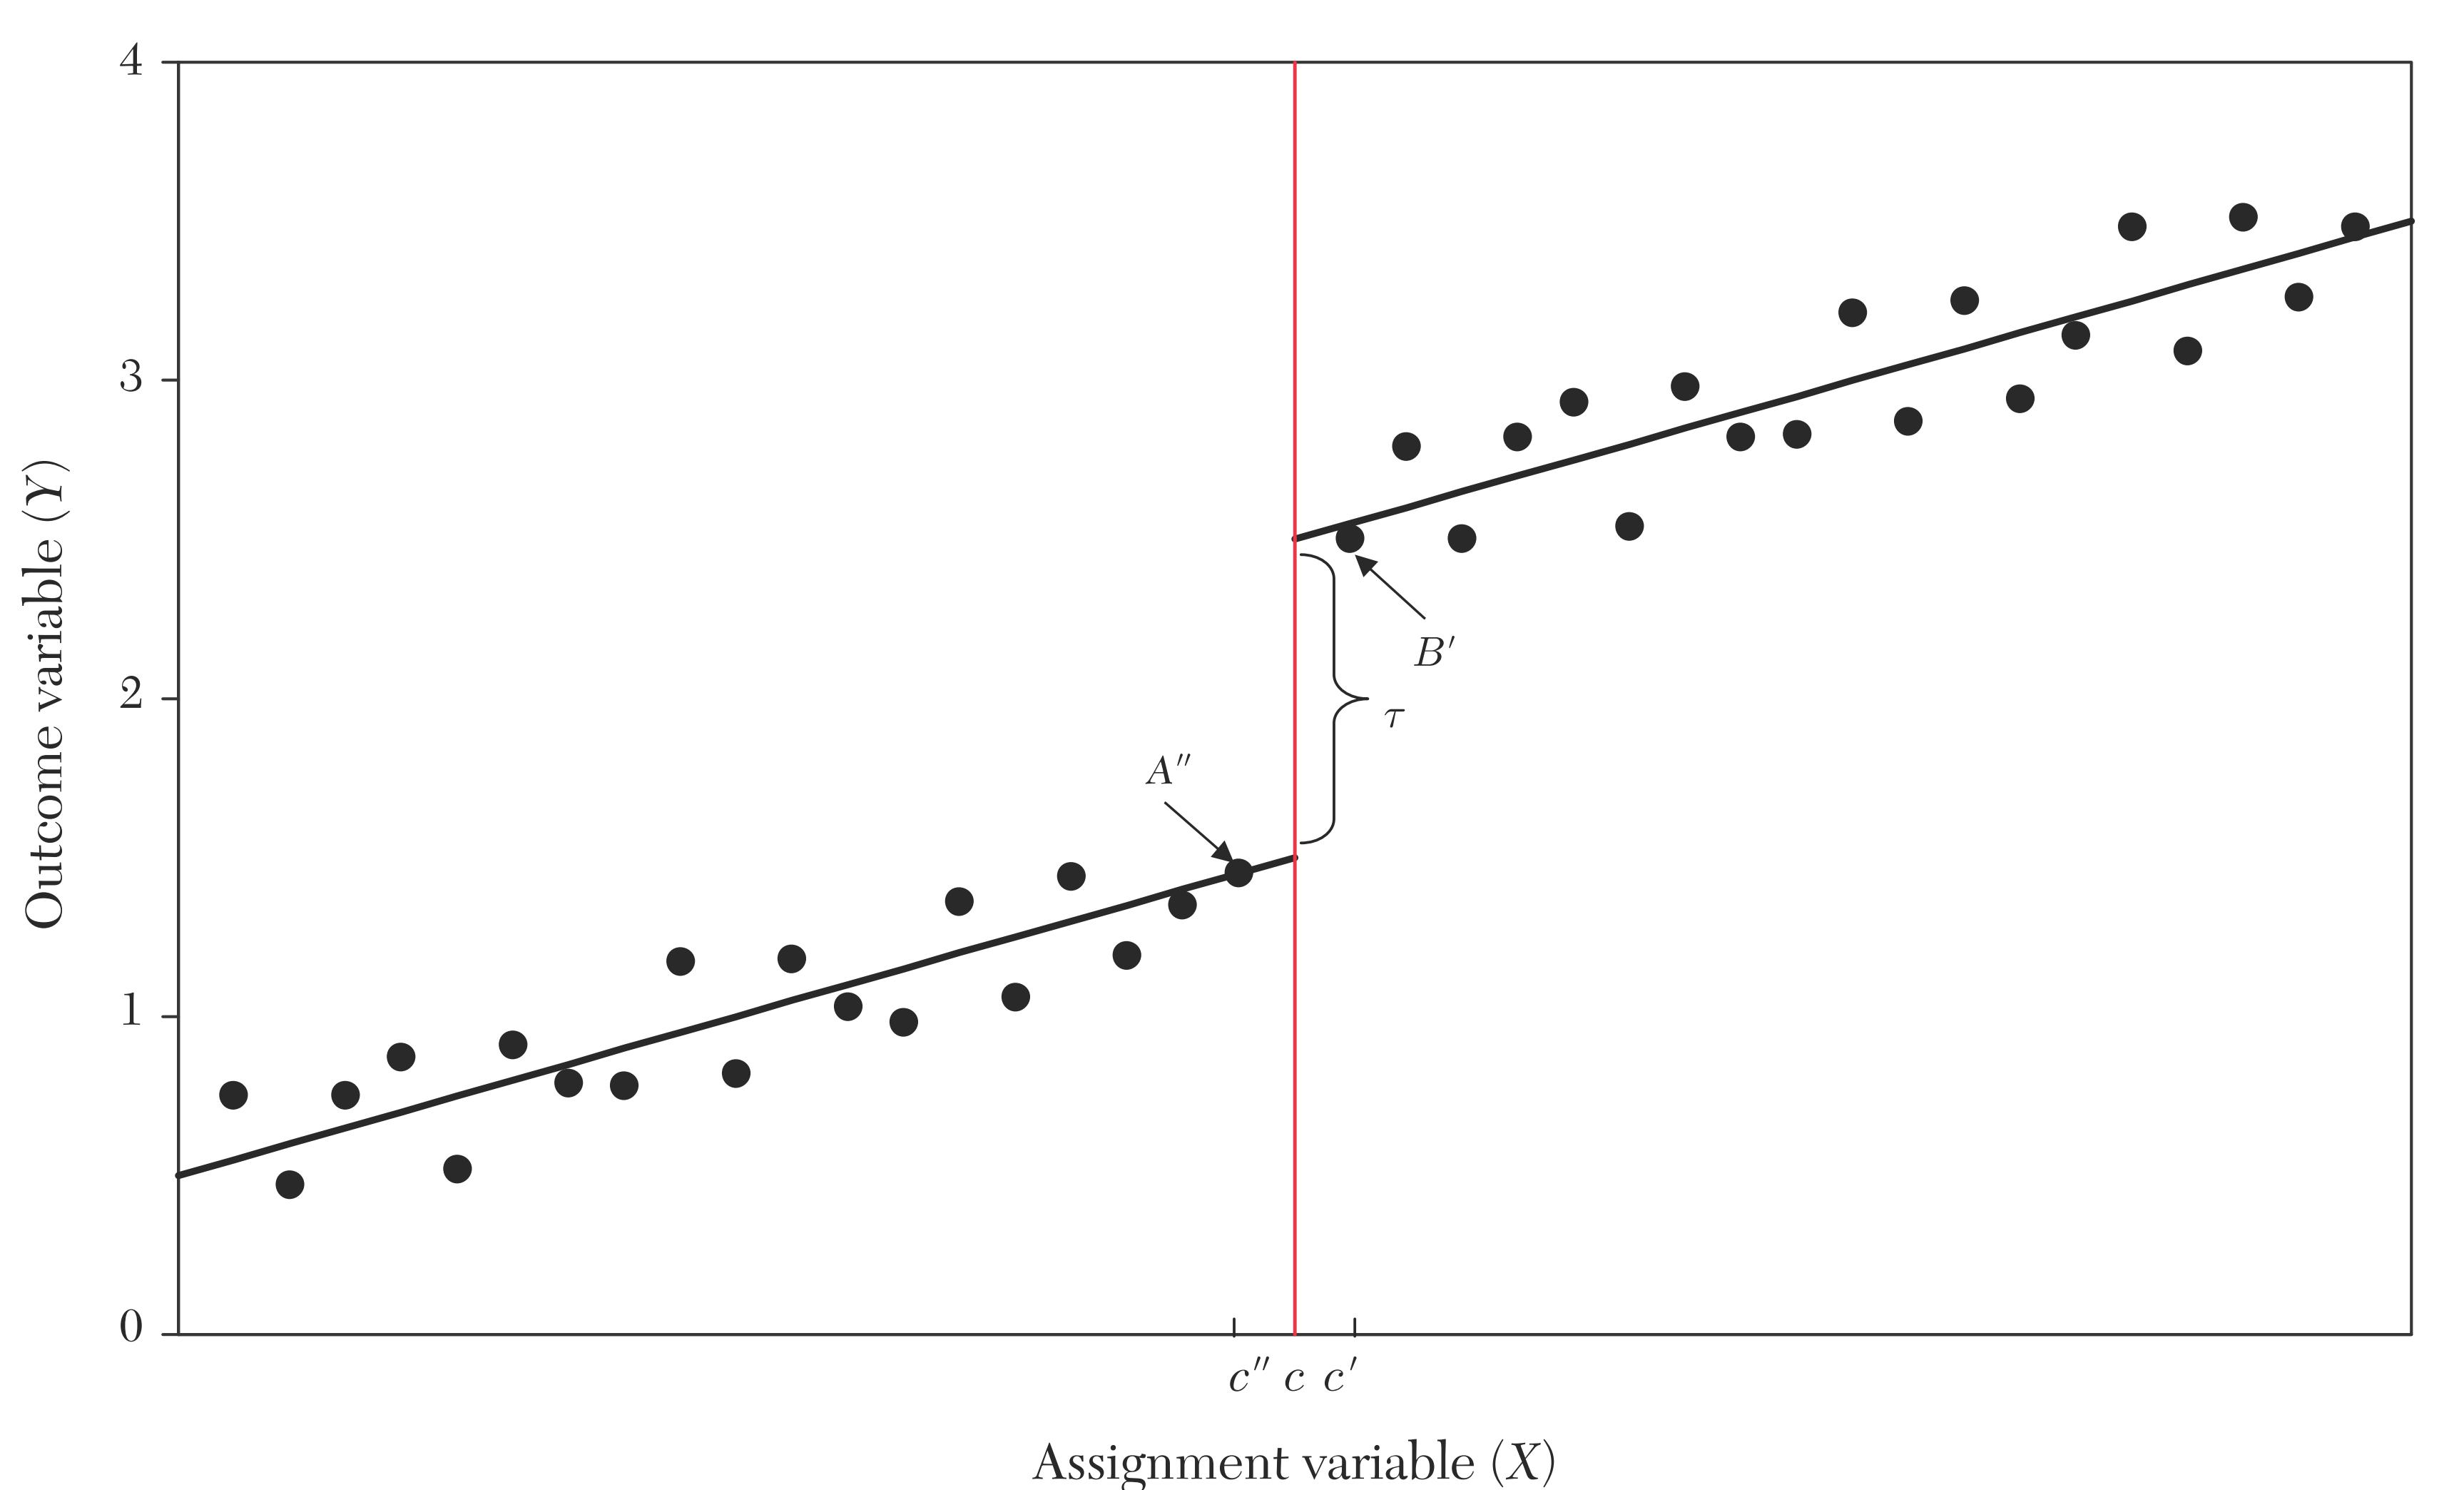
\includegraphics[width=1.0\textwidth]{figure/RD_score_f1.jpg}
	\end{figure}
	\begin{minipage}{0.9\linewidth}
		\fontsize{8}{8pt}\selectfont
		\emph{Source:} Lee and Lemieux (2010)
	\end{minipage}
\end{center}


\end{frame}







\begin{frame}{Main Idea of Regression Discontinuity Design}{A Motivating Example}

Mark Hoekstra (2009) ``\textbf{The Effect of Attending the Flagship State University on Earnings: A Discontinuity-Based Approach}" Review of Economics and Statistics

\begin{itemize}

%\item ``Where there is a cutoff there is a RD"
%\vspace{0.2cm}
%\item Fortunately, it is typical for selective schools and programs to use fairly strict grade cutoffs for admission
\item This paper demonstrates the above RD idea by examining the economic return of attending the most selective public state
university

\vspace{0.2cm}
\item In the United States, most schools used SAT (or ACT) scores in
their admission process
\vspace{0.2cm}
\item For example, the flagship state university considered here uses a strict cutoff based on SAT score and high school GPA

\end{itemize}
\end{frame}

\begin{frame}{Main Idea of Regression Discontinuity Design}{A Motivating Example}
\begin{itemize}

\item For the sake of simplicity, Hoekstra just focuses on the SAT score (adjusted depending on GPA)
\vspace{0.2cm}
\item The author is then able to match (using social security numbers) students applying to the flagship university in 1986-89 to their
administrative earnings data for 1998 to 2005
\vspace{0.2cm}
\item As in any good RD study, pictures tell it all, so let's just focus on
those

\end{itemize}
\end{frame}



\begin{frame}{SAT Score and Enrollment}

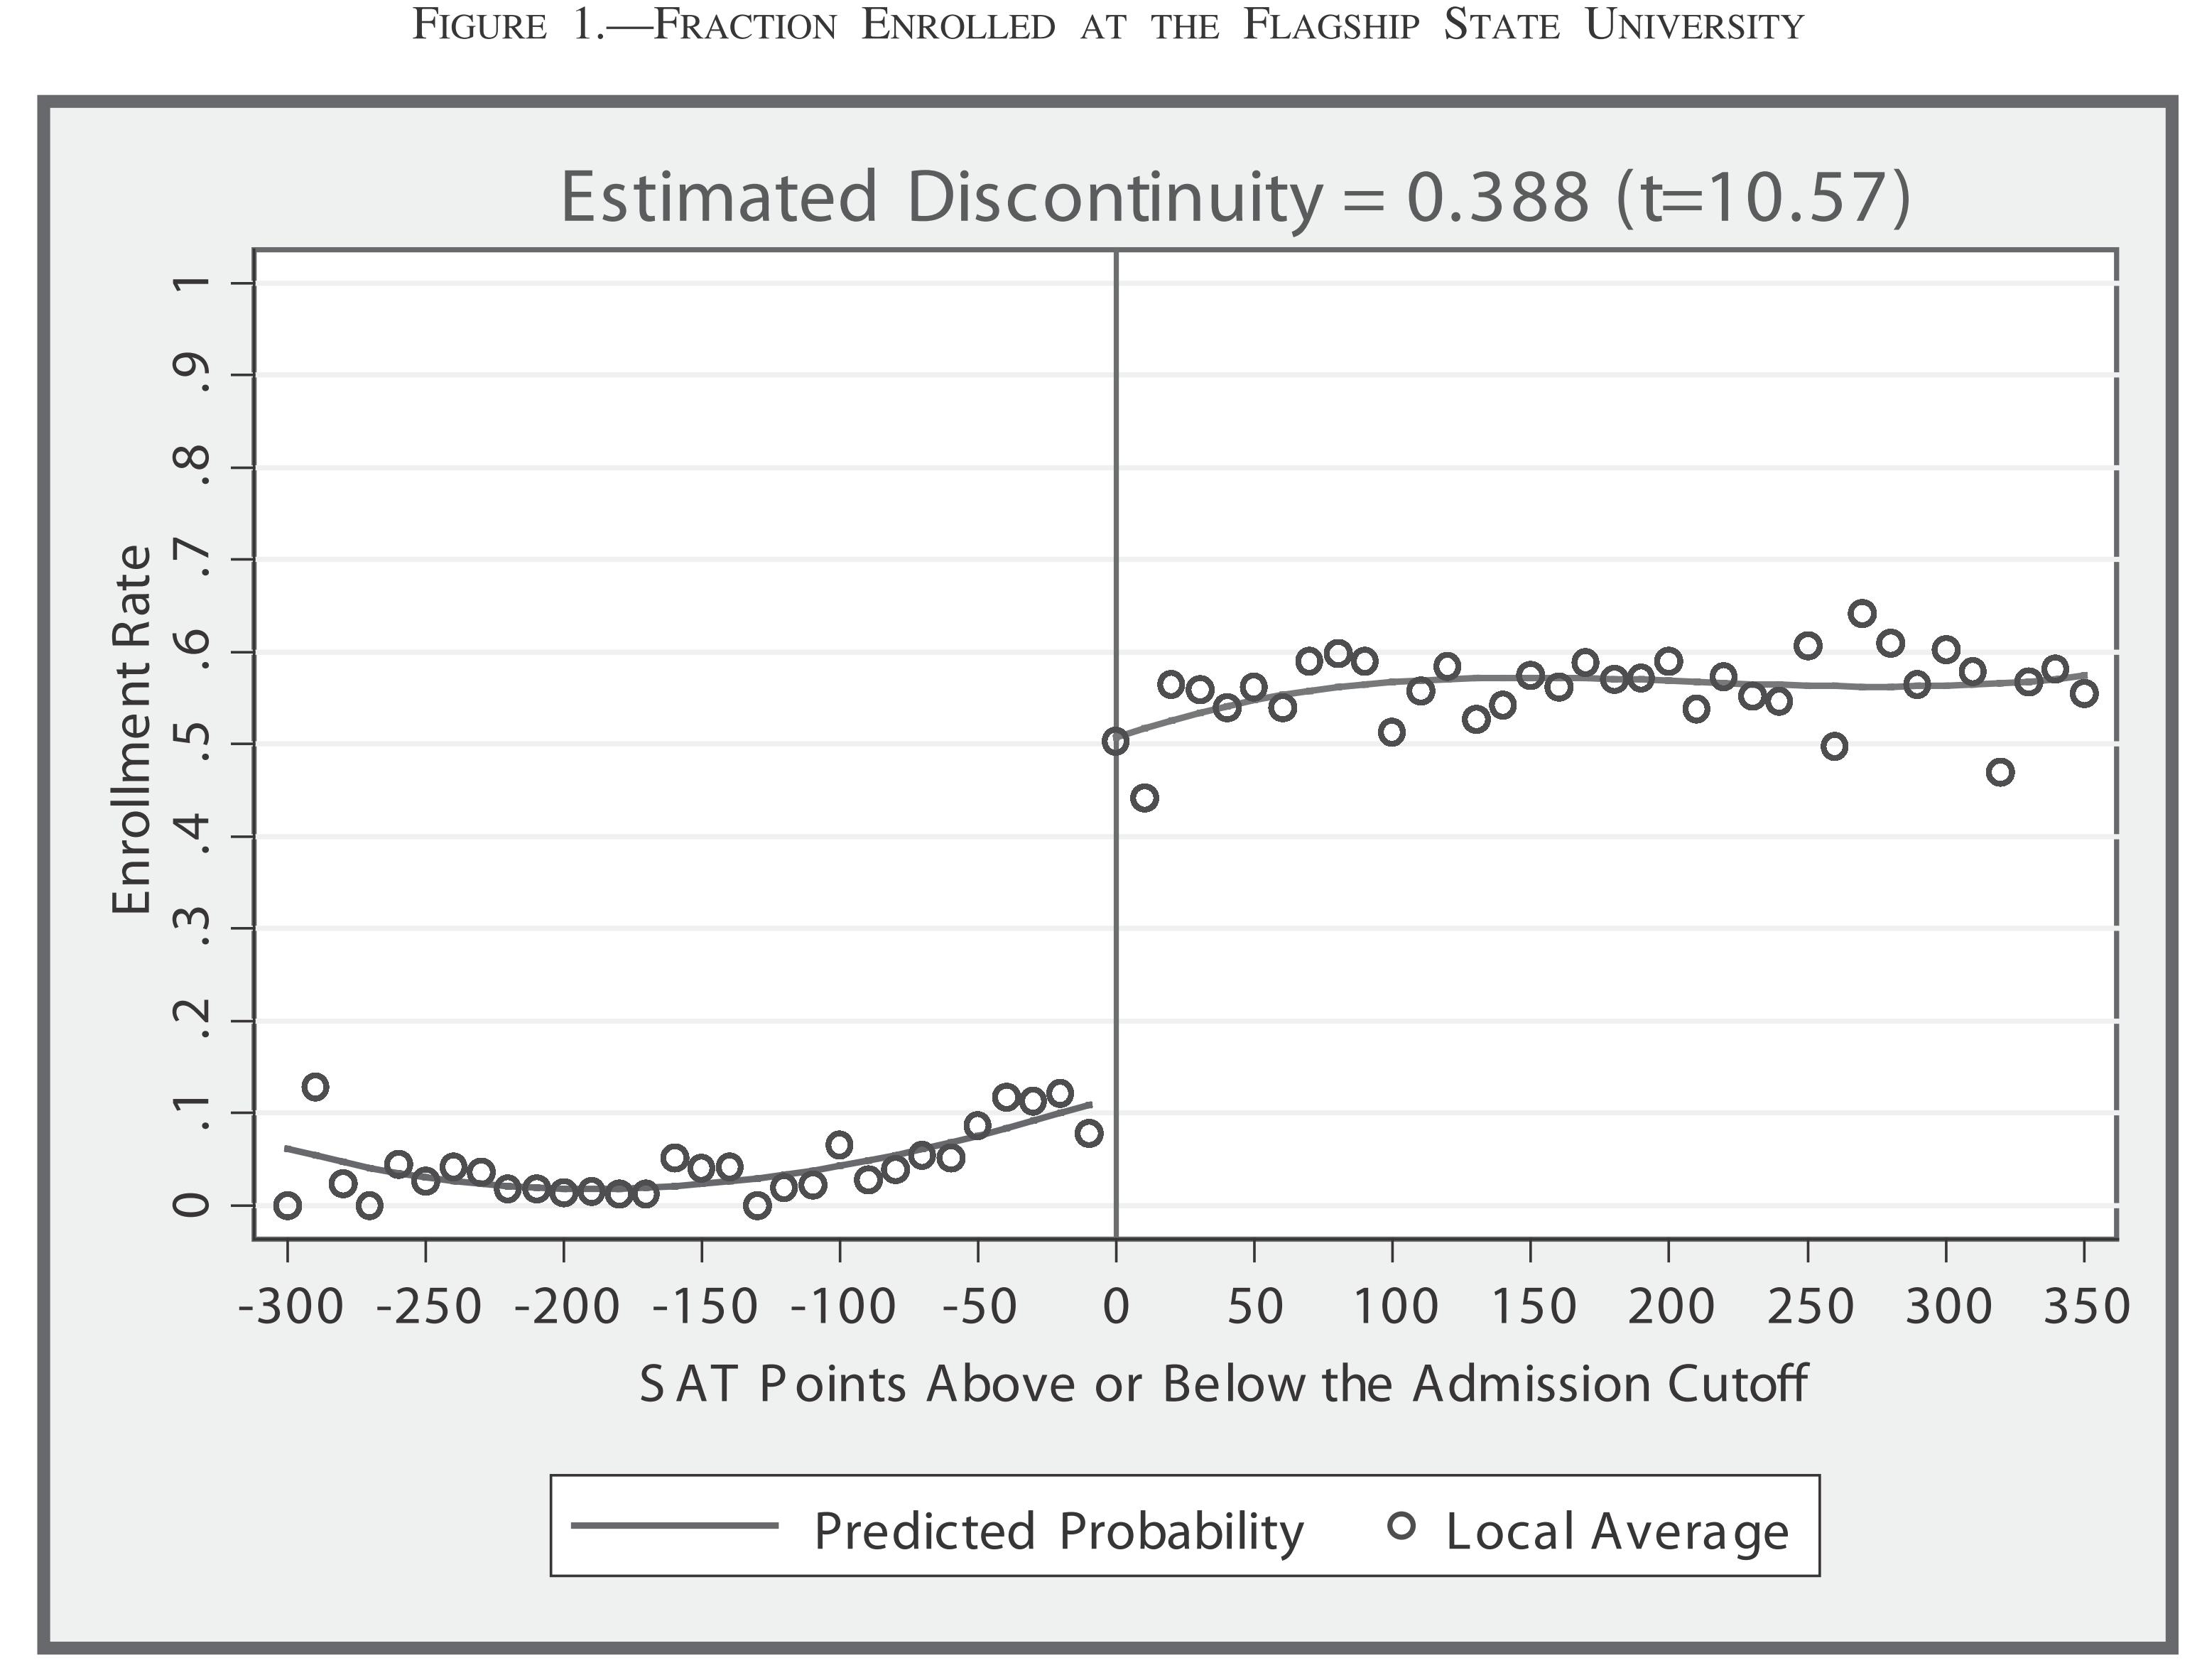
\includegraphics[width=1.0\textwidth]{figure/college_f1.jpg}


\end{frame}



\begin{frame}{SAT Score and Earnings}

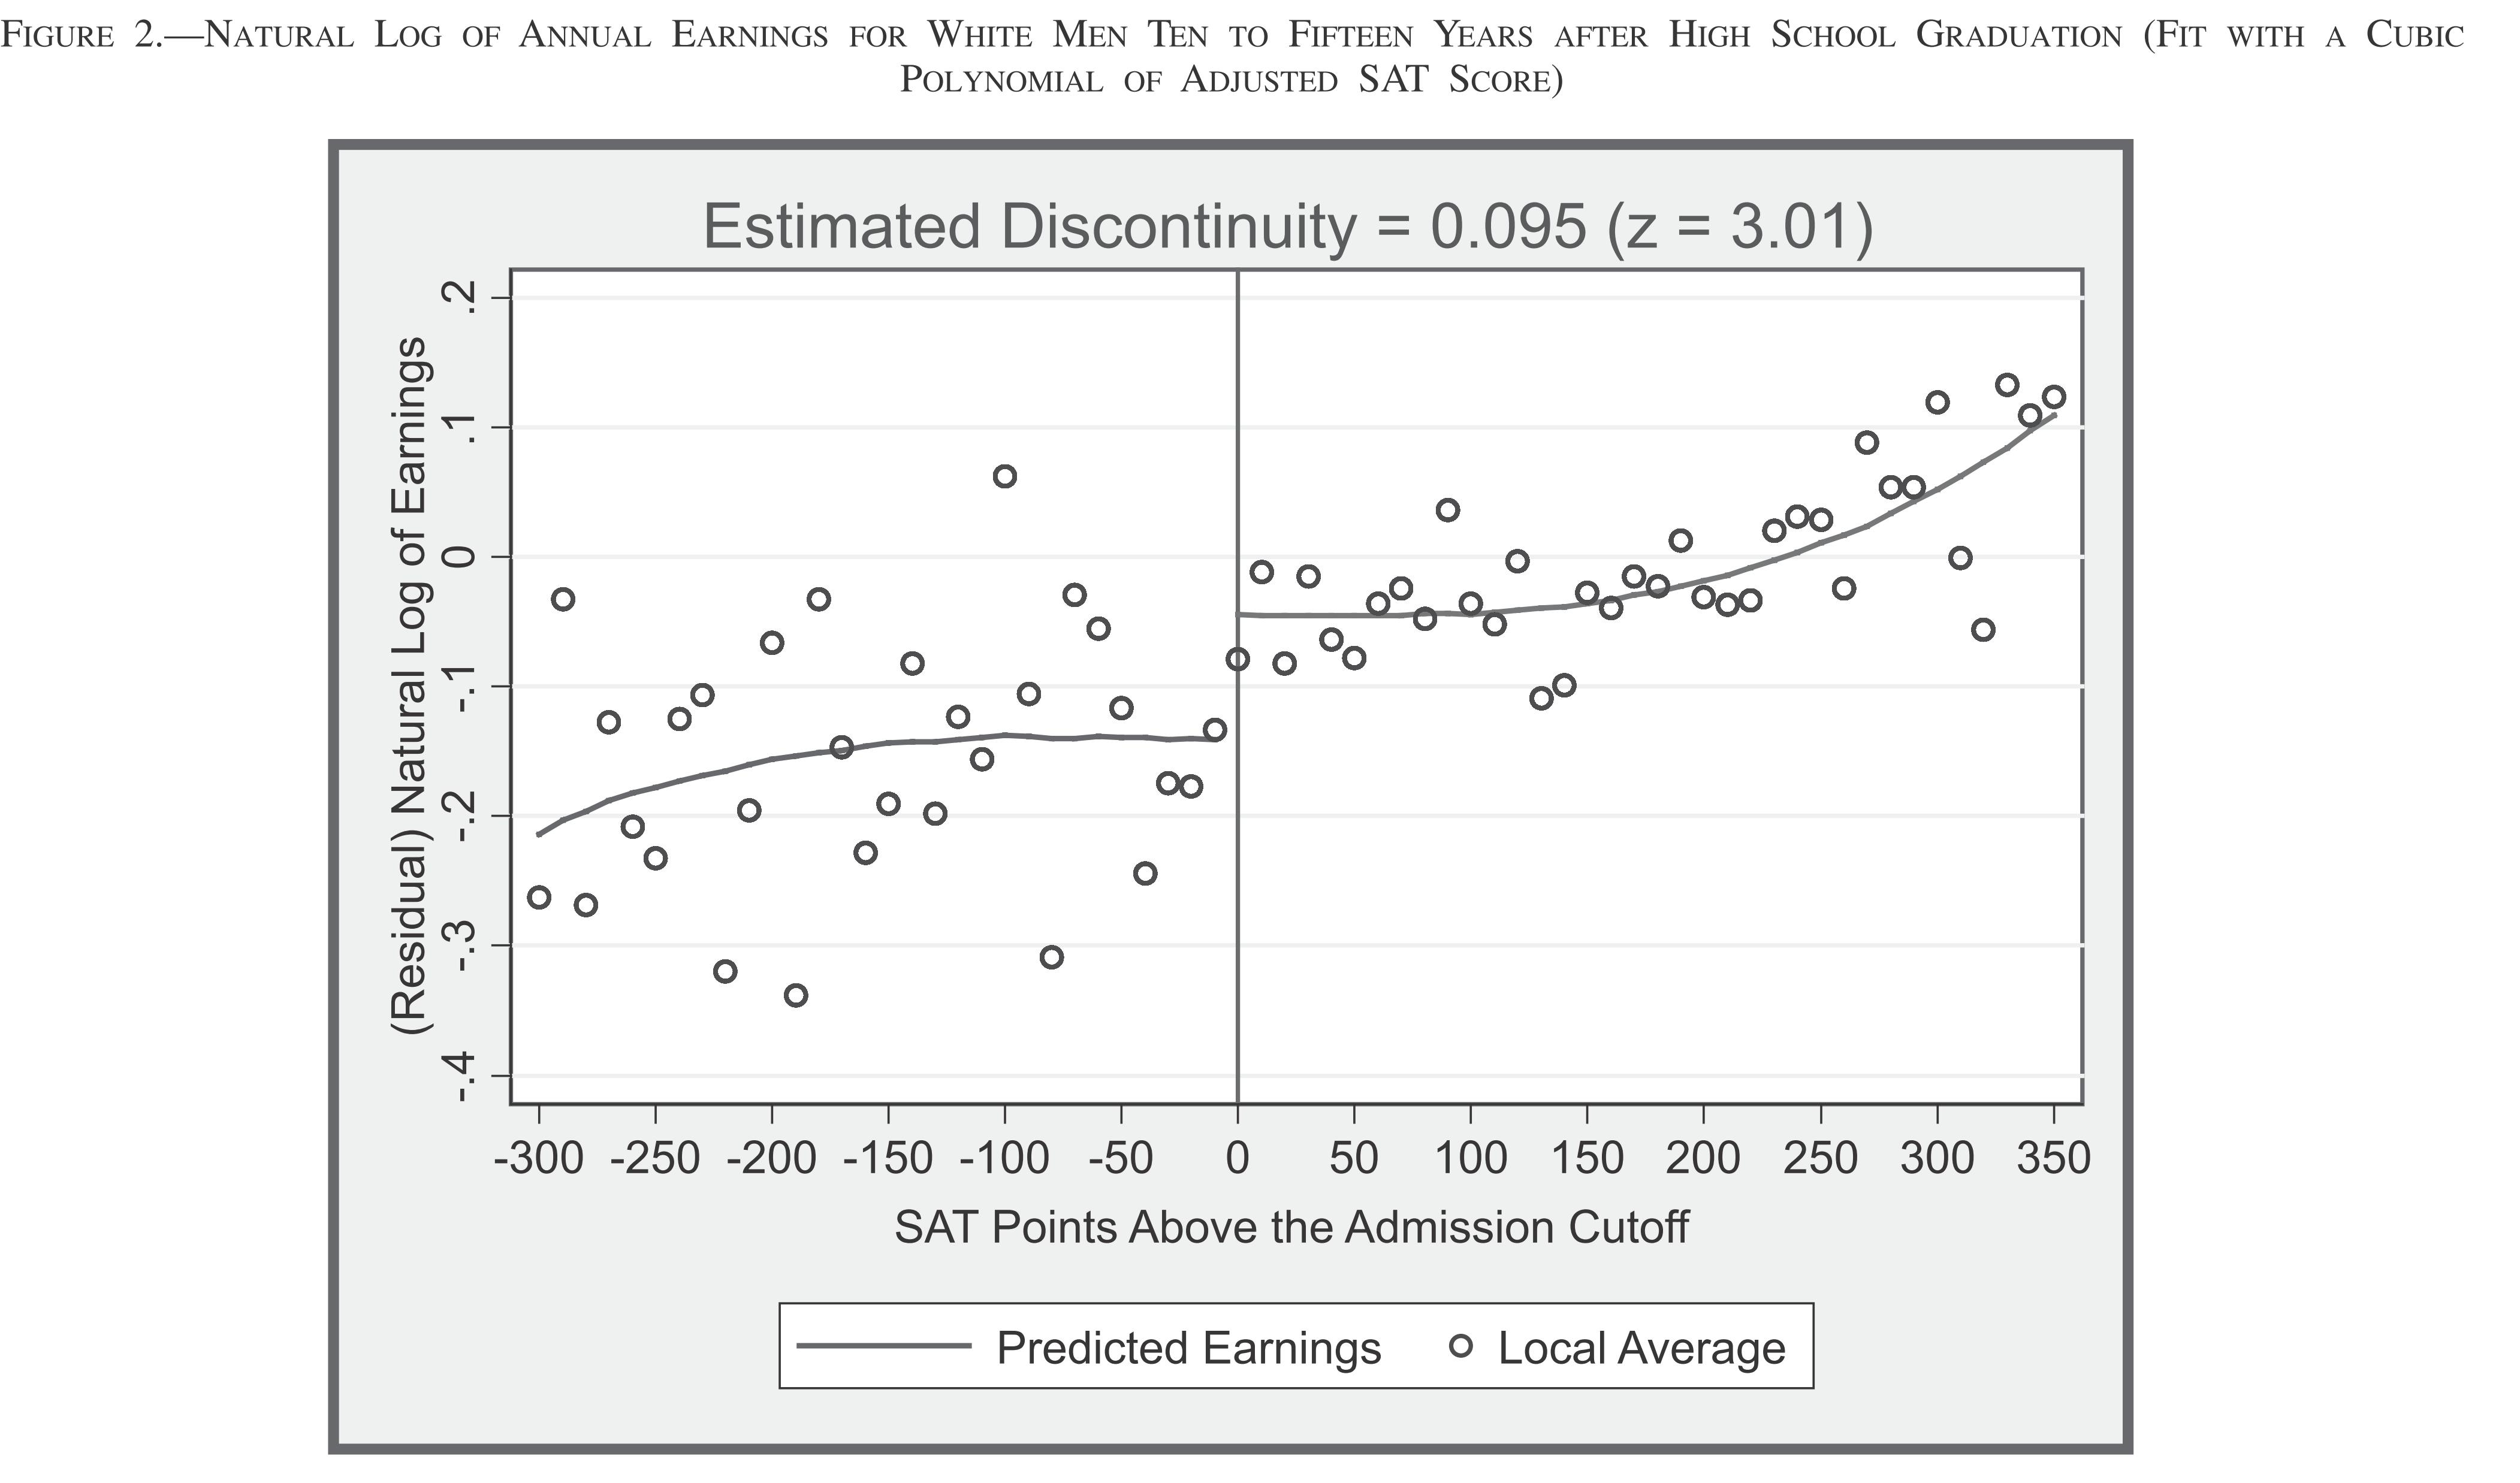
\includegraphics[width=1.0\textwidth]{figure/college_f2.jpg}


\end{frame}



\begin{frame}{More Examples}{}
\begin{itemize}

\item \textbf{Where there is a cutoff there is a RD}

\end{itemize}
\end{frame}




\begin{frame}{Public Health}{The Effect of Health Intervention}

Prashant Bharadwaj, Katrine Vellesen Løken, and
Christopher Neilson (2013) ``\textbf{Early Life Health Interventions and Academic Achievement}" AER

\begin{itemize}

\item The effect of \textbf{health intervention} in early childhood on \textbf{later life outcomes}
\vspace{0.2cm}
\item \textbf{Selection bias}: children who need health intervention in early childhood could be very sick and might have bad later life outcome (e.g. low educational attachment)

\end{itemize}
\end{frame}




\begin{frame}{Public Health}{The Effect of Health Intervention}
\begin{itemize}


\item \textbf{RDD solution}: 
\vspace{0.2cm}
\begin{itemize}
\item Infants with a birth weight below \textbf{1500 grams} were eligible for additional healthcare while those with a birth weight just above the cutoff were not eligible
\vspace{0.2cm}
\end{itemize}
\item Compares mortality rates and academic achievement between those infants \textbf{just below and above the cutoff of 1500 grams} 
\end{itemize}
\end{frame}




\begin{frame}{}

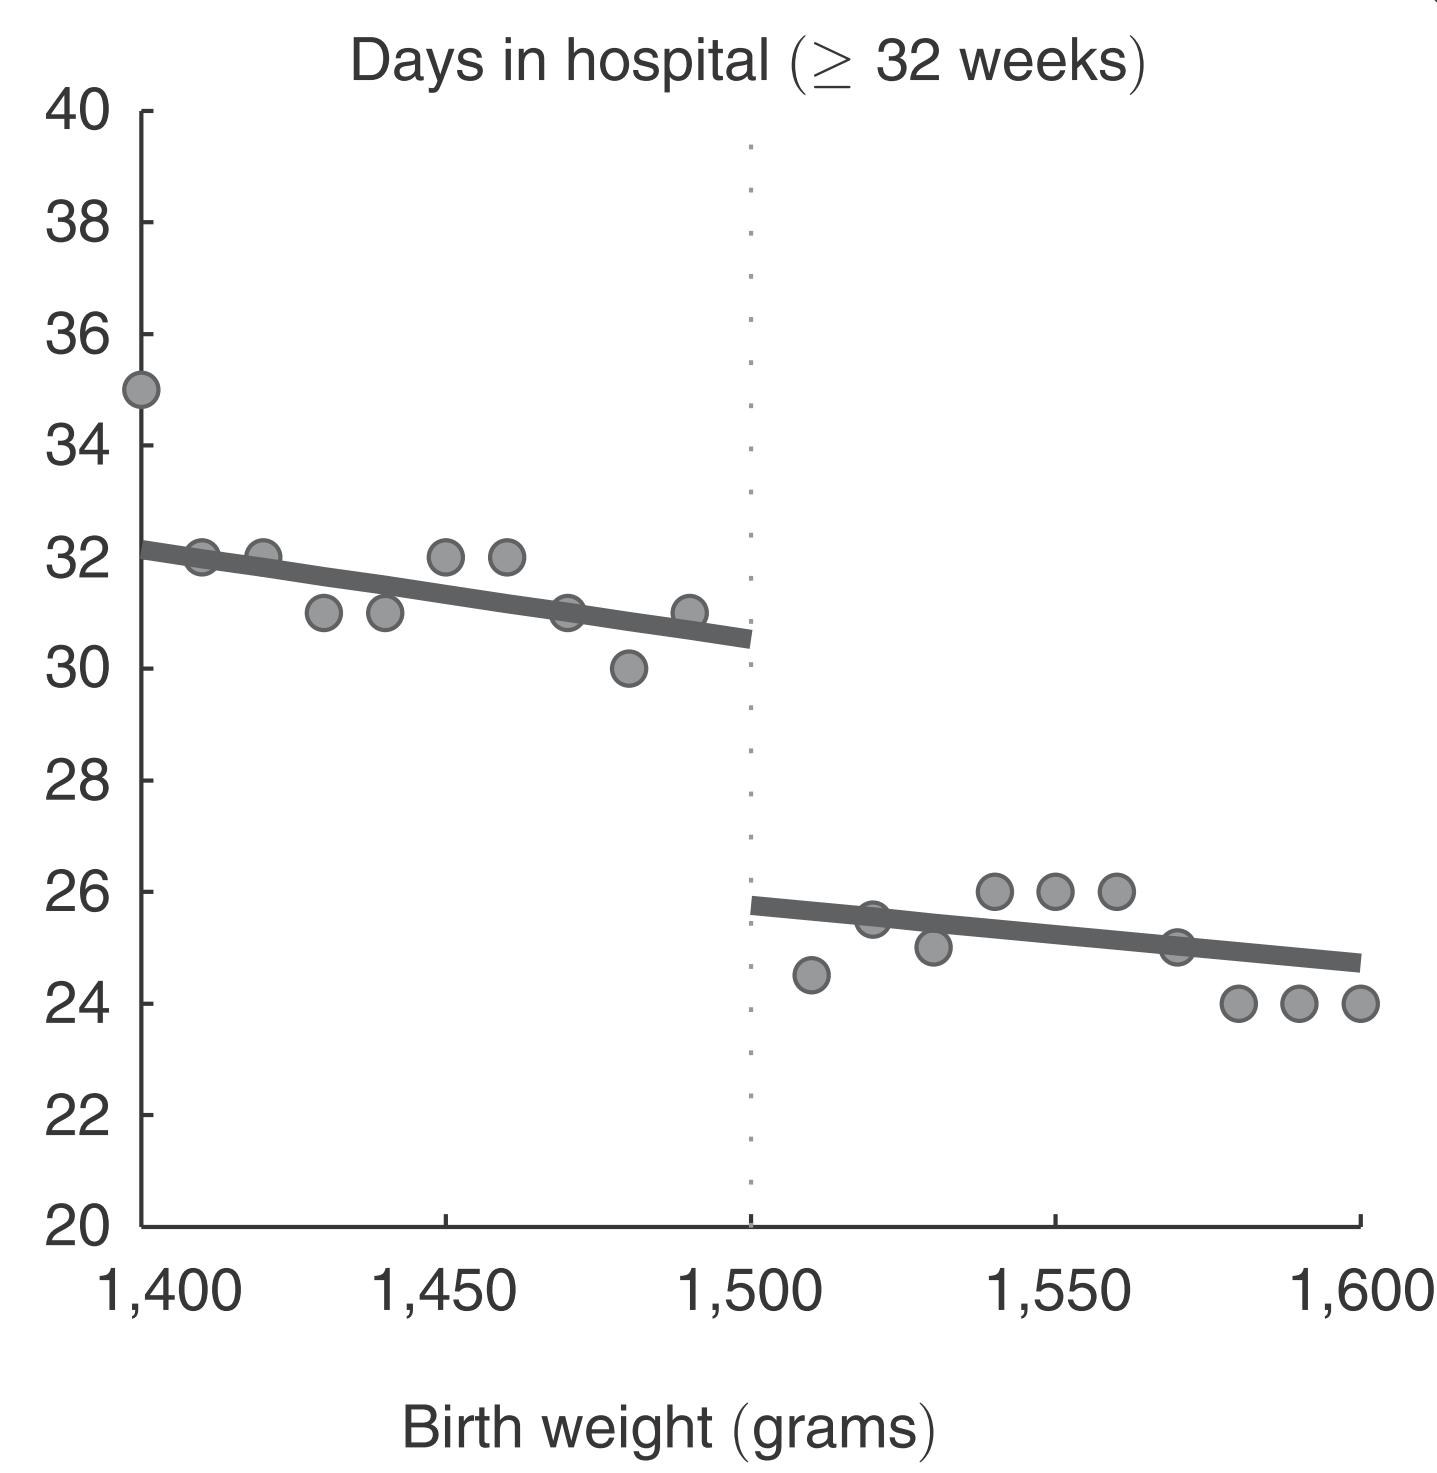
\includegraphics[width=0.7\textwidth]{figure/RD_health_f1.jpg}


\end{frame}


\begin{frame}{}

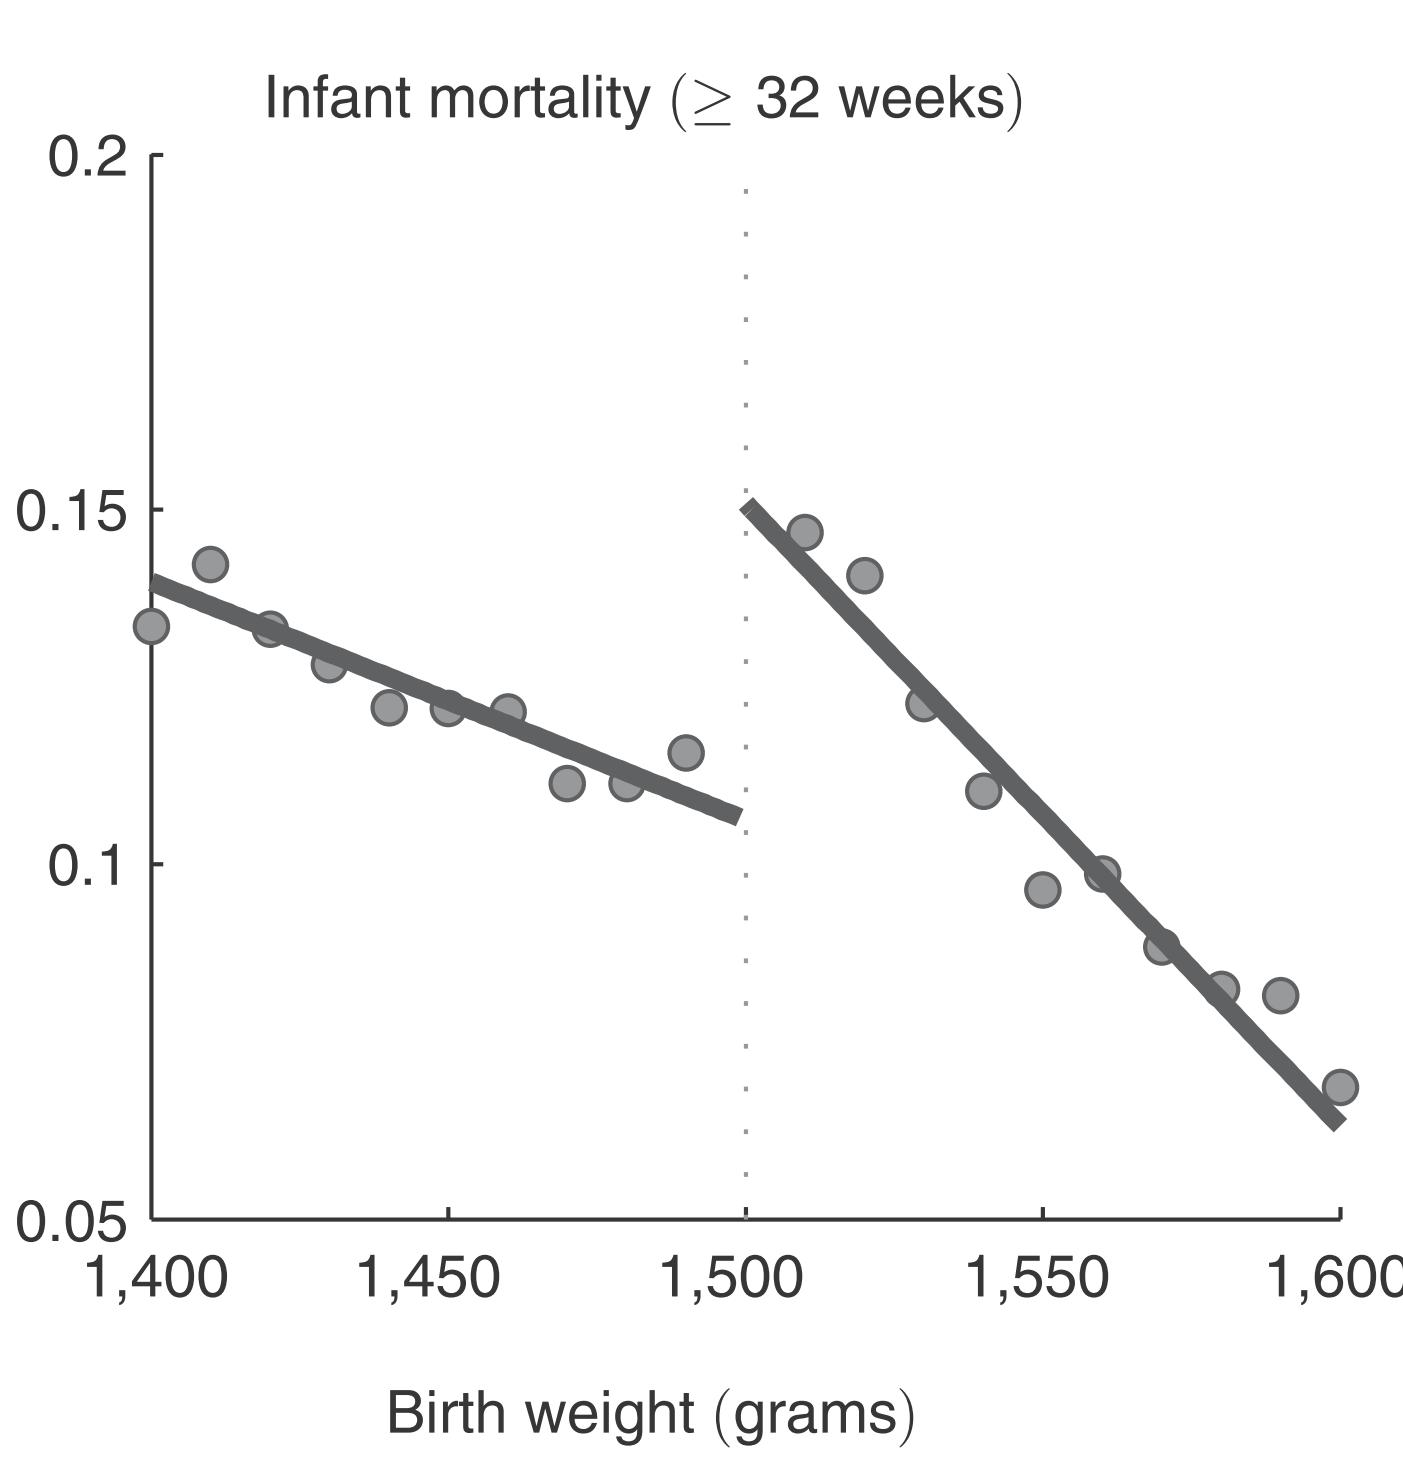
\includegraphics[width=0.7\textwidth]{figure/RD_health_f2.jpg}


\end{frame}


\begin{frame}{}

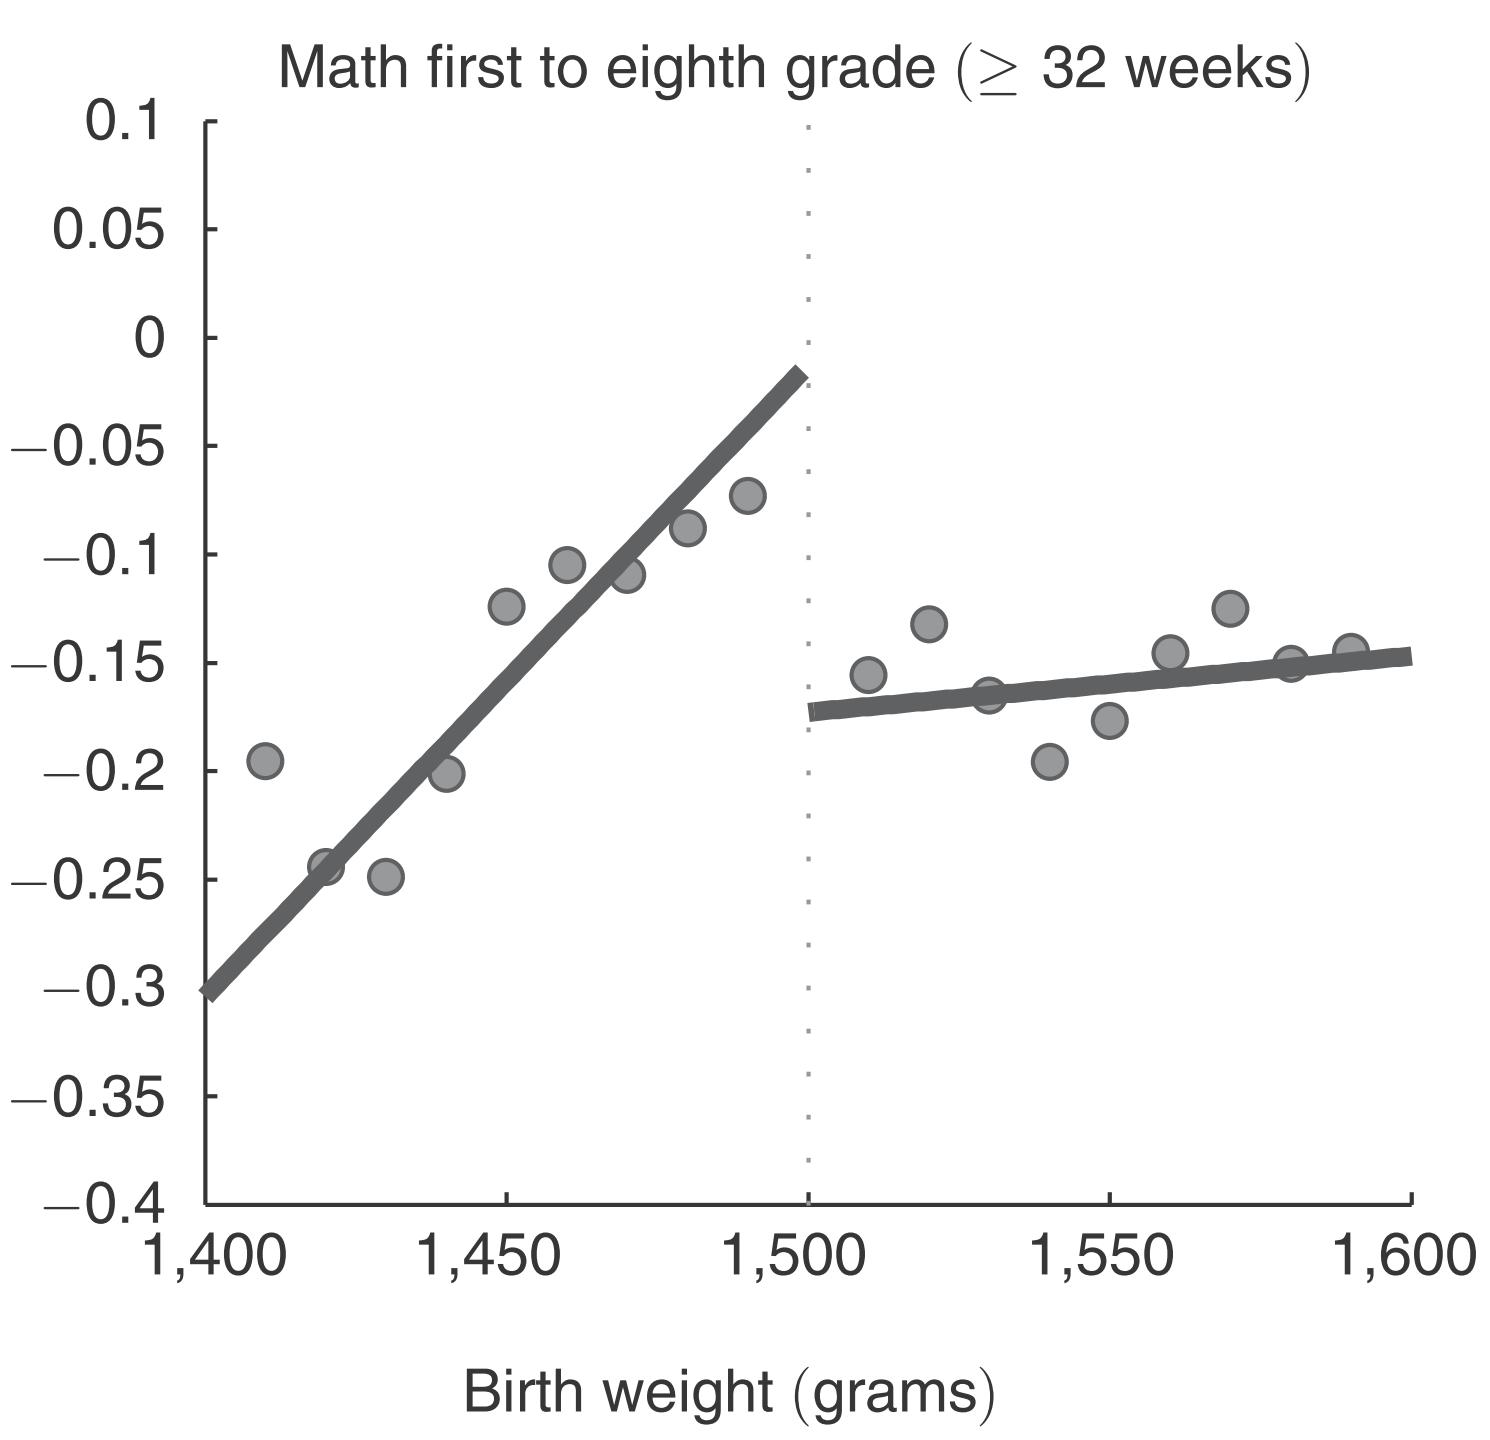
\includegraphics[width=0.7\textwidth]{figure/RD_health_f3.jpg}


\end{frame}


\begin{frame}{Political Science}{The Effect of Incumbency}

David Lee (2007) ``\textbf{Randomized Experiments from Non-random Selection in U.S. House Elections}" Journal of Econometrics

\begin{itemize}

\item  Does \textbf{political incumbency} provide an \textbf{electoral advantage}
\vspace{0.2cm}
\item \textbf{Selection bias}: people who win election (incumbency) should be more popular

\end{itemize}
\end{frame}




\begin{frame}{Political Science}{The Effect of Incumbency}
\begin{itemize}
	
	\item \textbf{RDD solution}: 
	\vspace{0.2cm}
	\begin{itemize}
		\item Candidates who just \textbf{barely won} an election (barely became the incumbent) are likely to be ex ante comparable in all other ways to candidates who \textbf{barely lost}
		\vspace{0.2cm}
		\item So their differential electoral outcomes in the \textbf{next election} should represent a true \textbf{incumbency advantage}
	\end{itemize}
\end{itemize}
\end{frame}



\begin{frame}{}

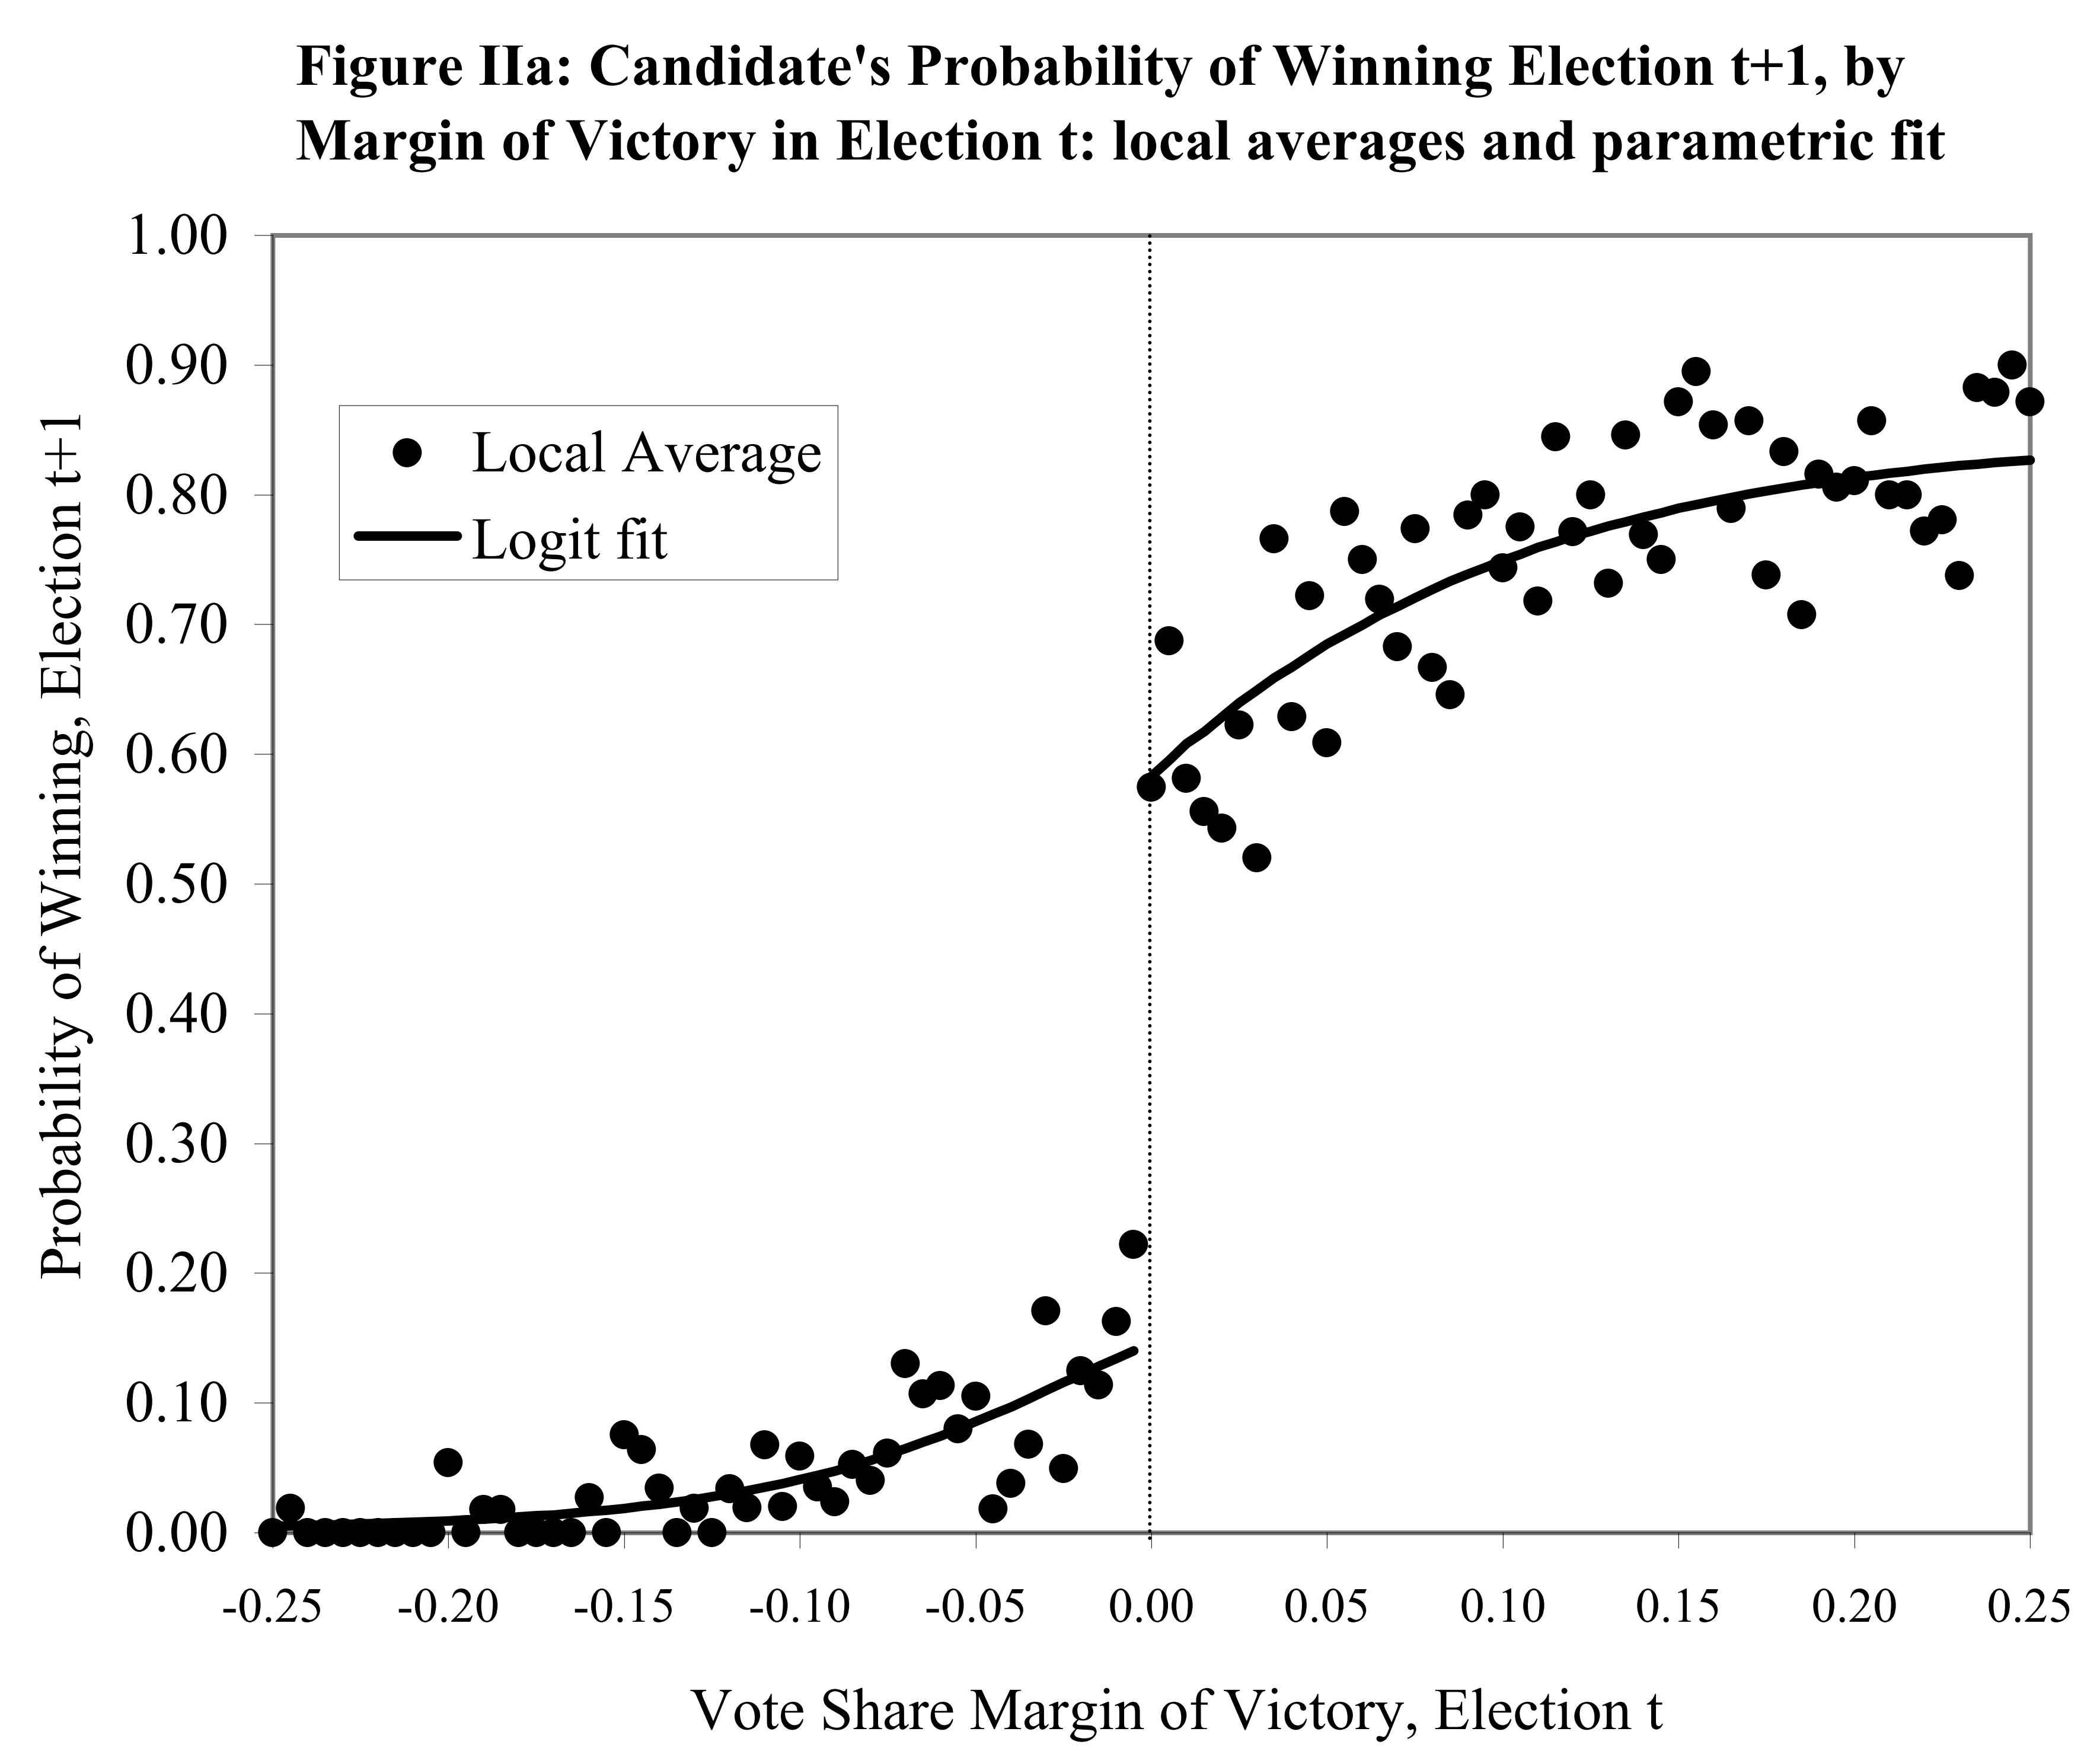
\includegraphics[width=0.9\textwidth]{figure/RD_poli_f1.jpg}


\end{frame}



\begin{frame}{Labor Economics}{Spatial Regression Discontinuity}
	Rafael Lalive (2008), ``\textbf{How do extended benefits affect unemployment duration?
		A regression discontinuity approach}", Journal of Econometrics
	\begin{itemize}
		\vspace{0.2cm}
		\item This paper studies a targeted program that extends the maximum duration of unemployment benefits from 30 weeks to 209 weeks in Austria
		\vspace{0.2cm}
		\item Sharp discontinuities in treatment assignment at age 50 and at the border between eligible regions and control regions identify the effect of \textbf{extended benefits} on \textbf{unemployment duration}
	\end{itemize}
\end{frame}


\begin{frame}{Labor Economics}{Spatial Regression Discontinuity}
	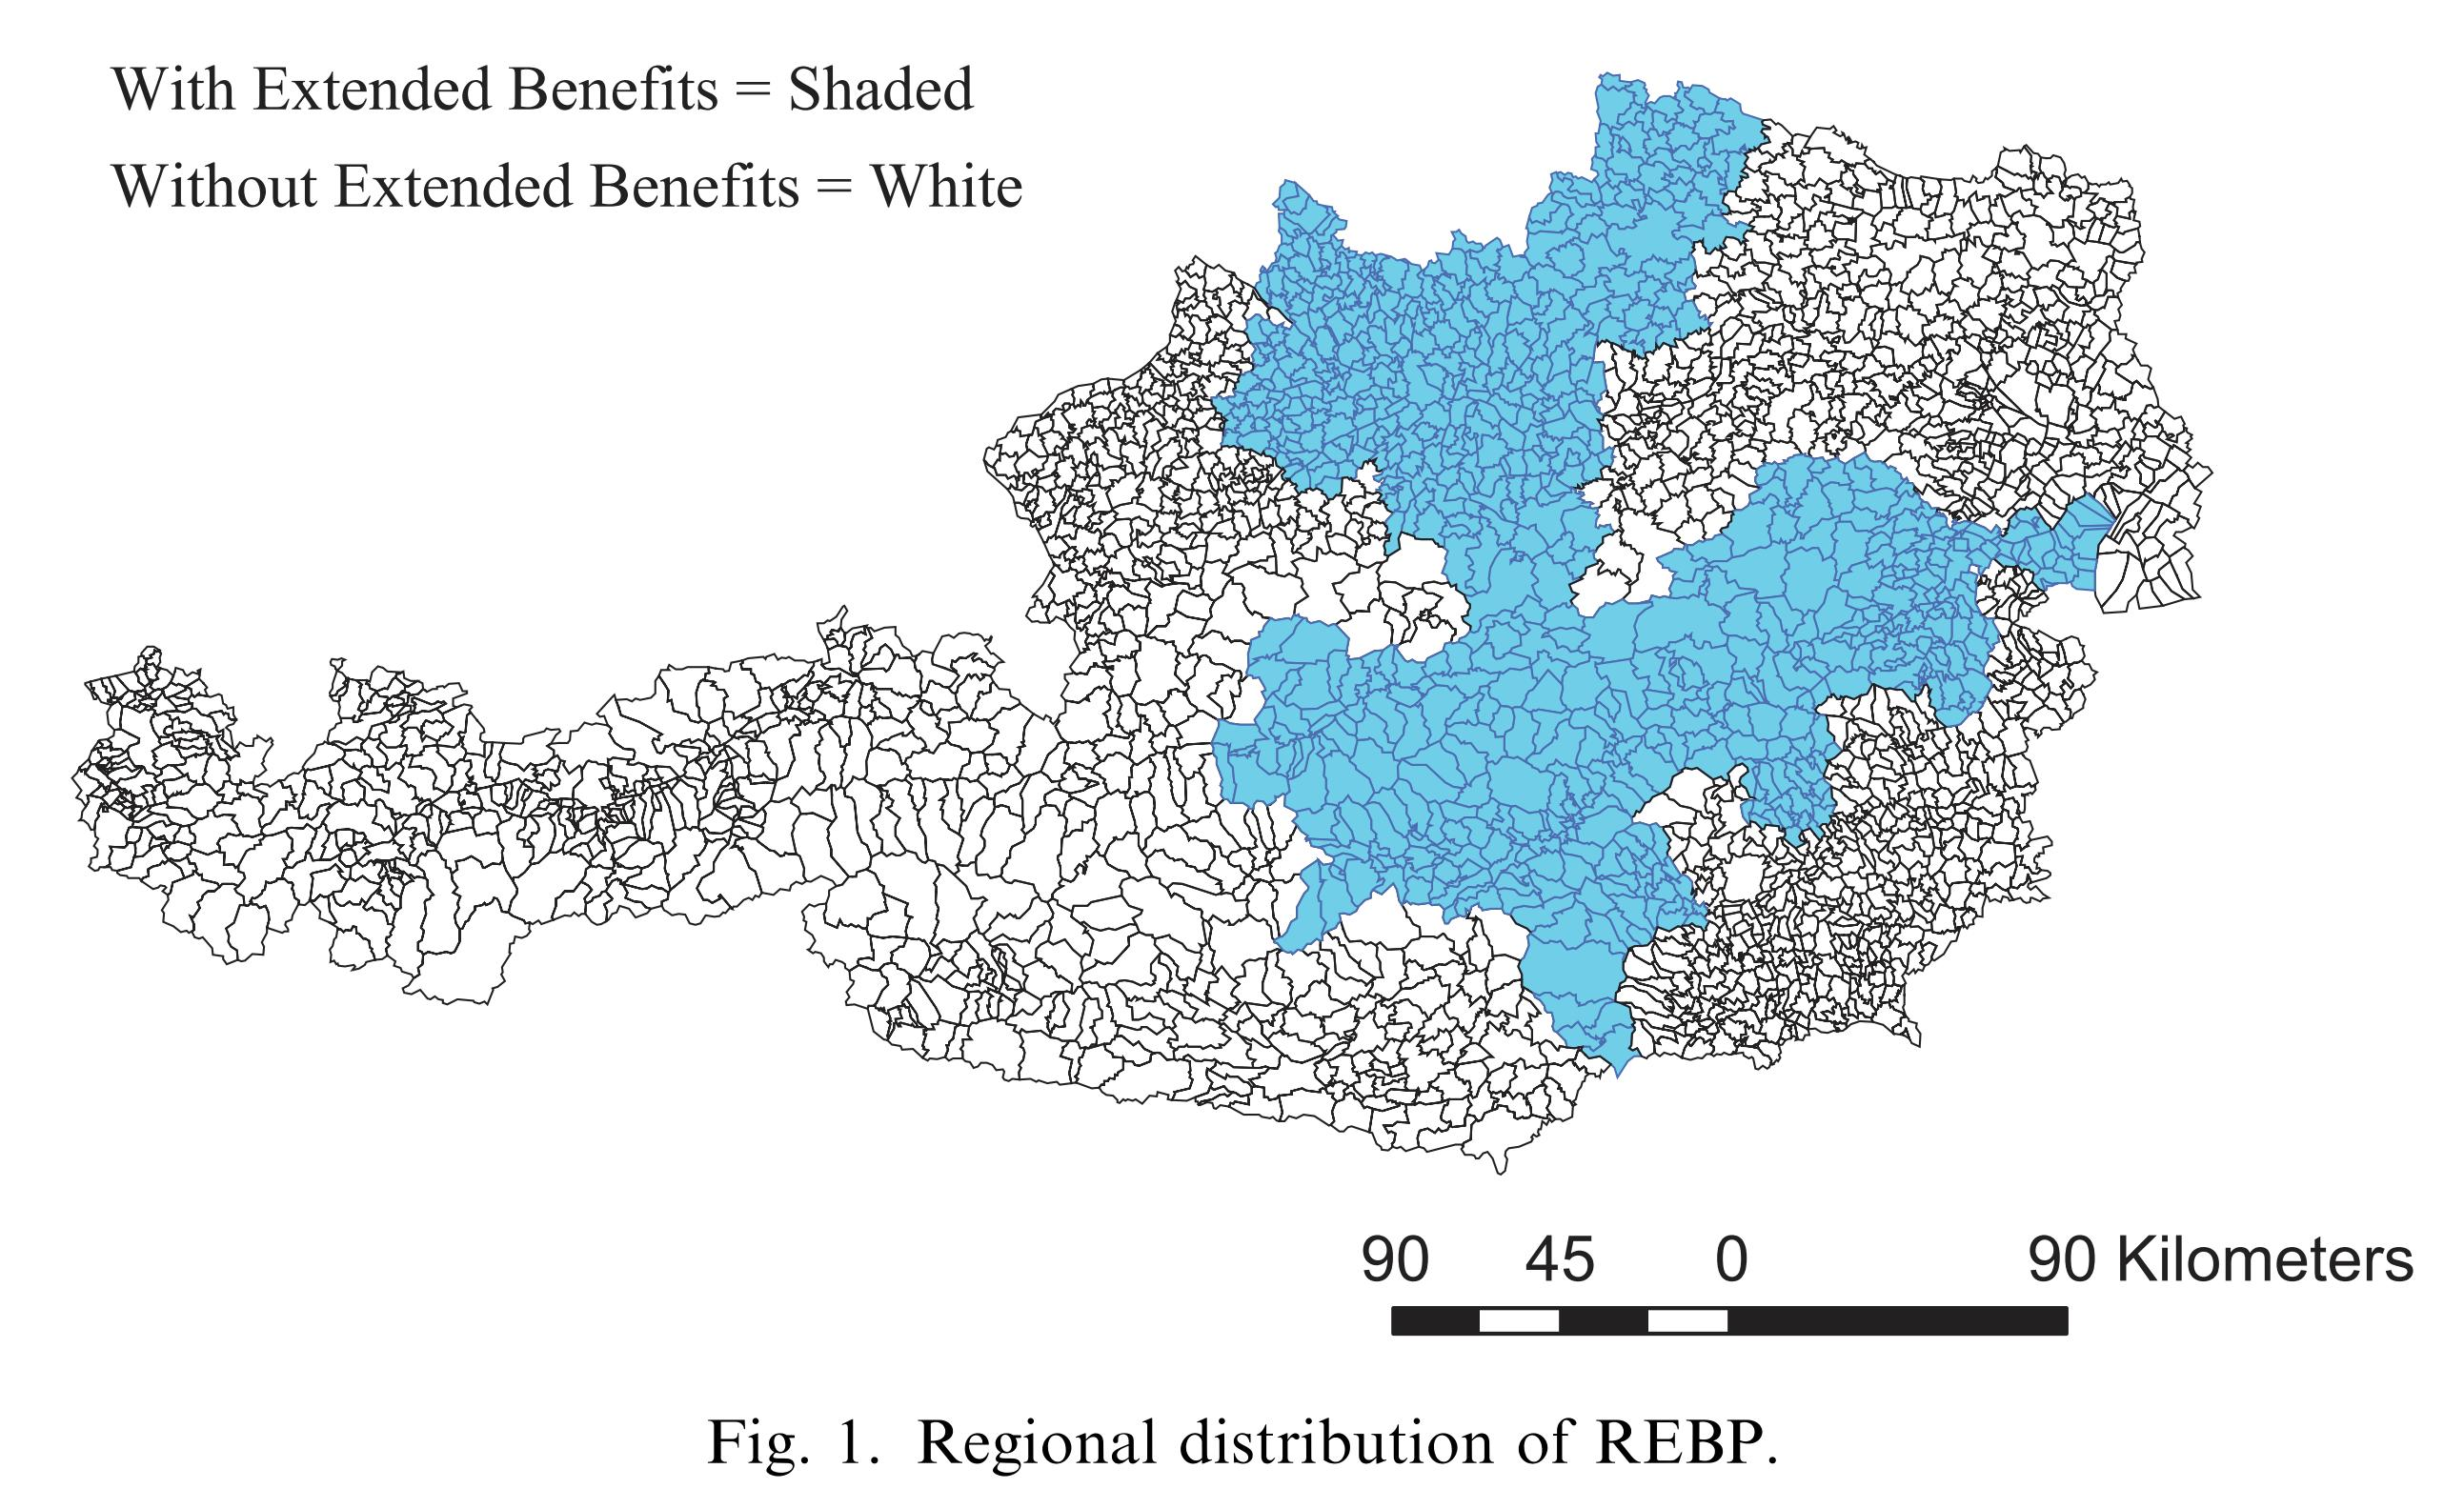
\includegraphics[width=.90\textwidth]{figure/srd_ui_f1.jpg}
	
\end{frame}


\begin{frame}{Labor Economics}{Spatial Regression Discontinuity}
	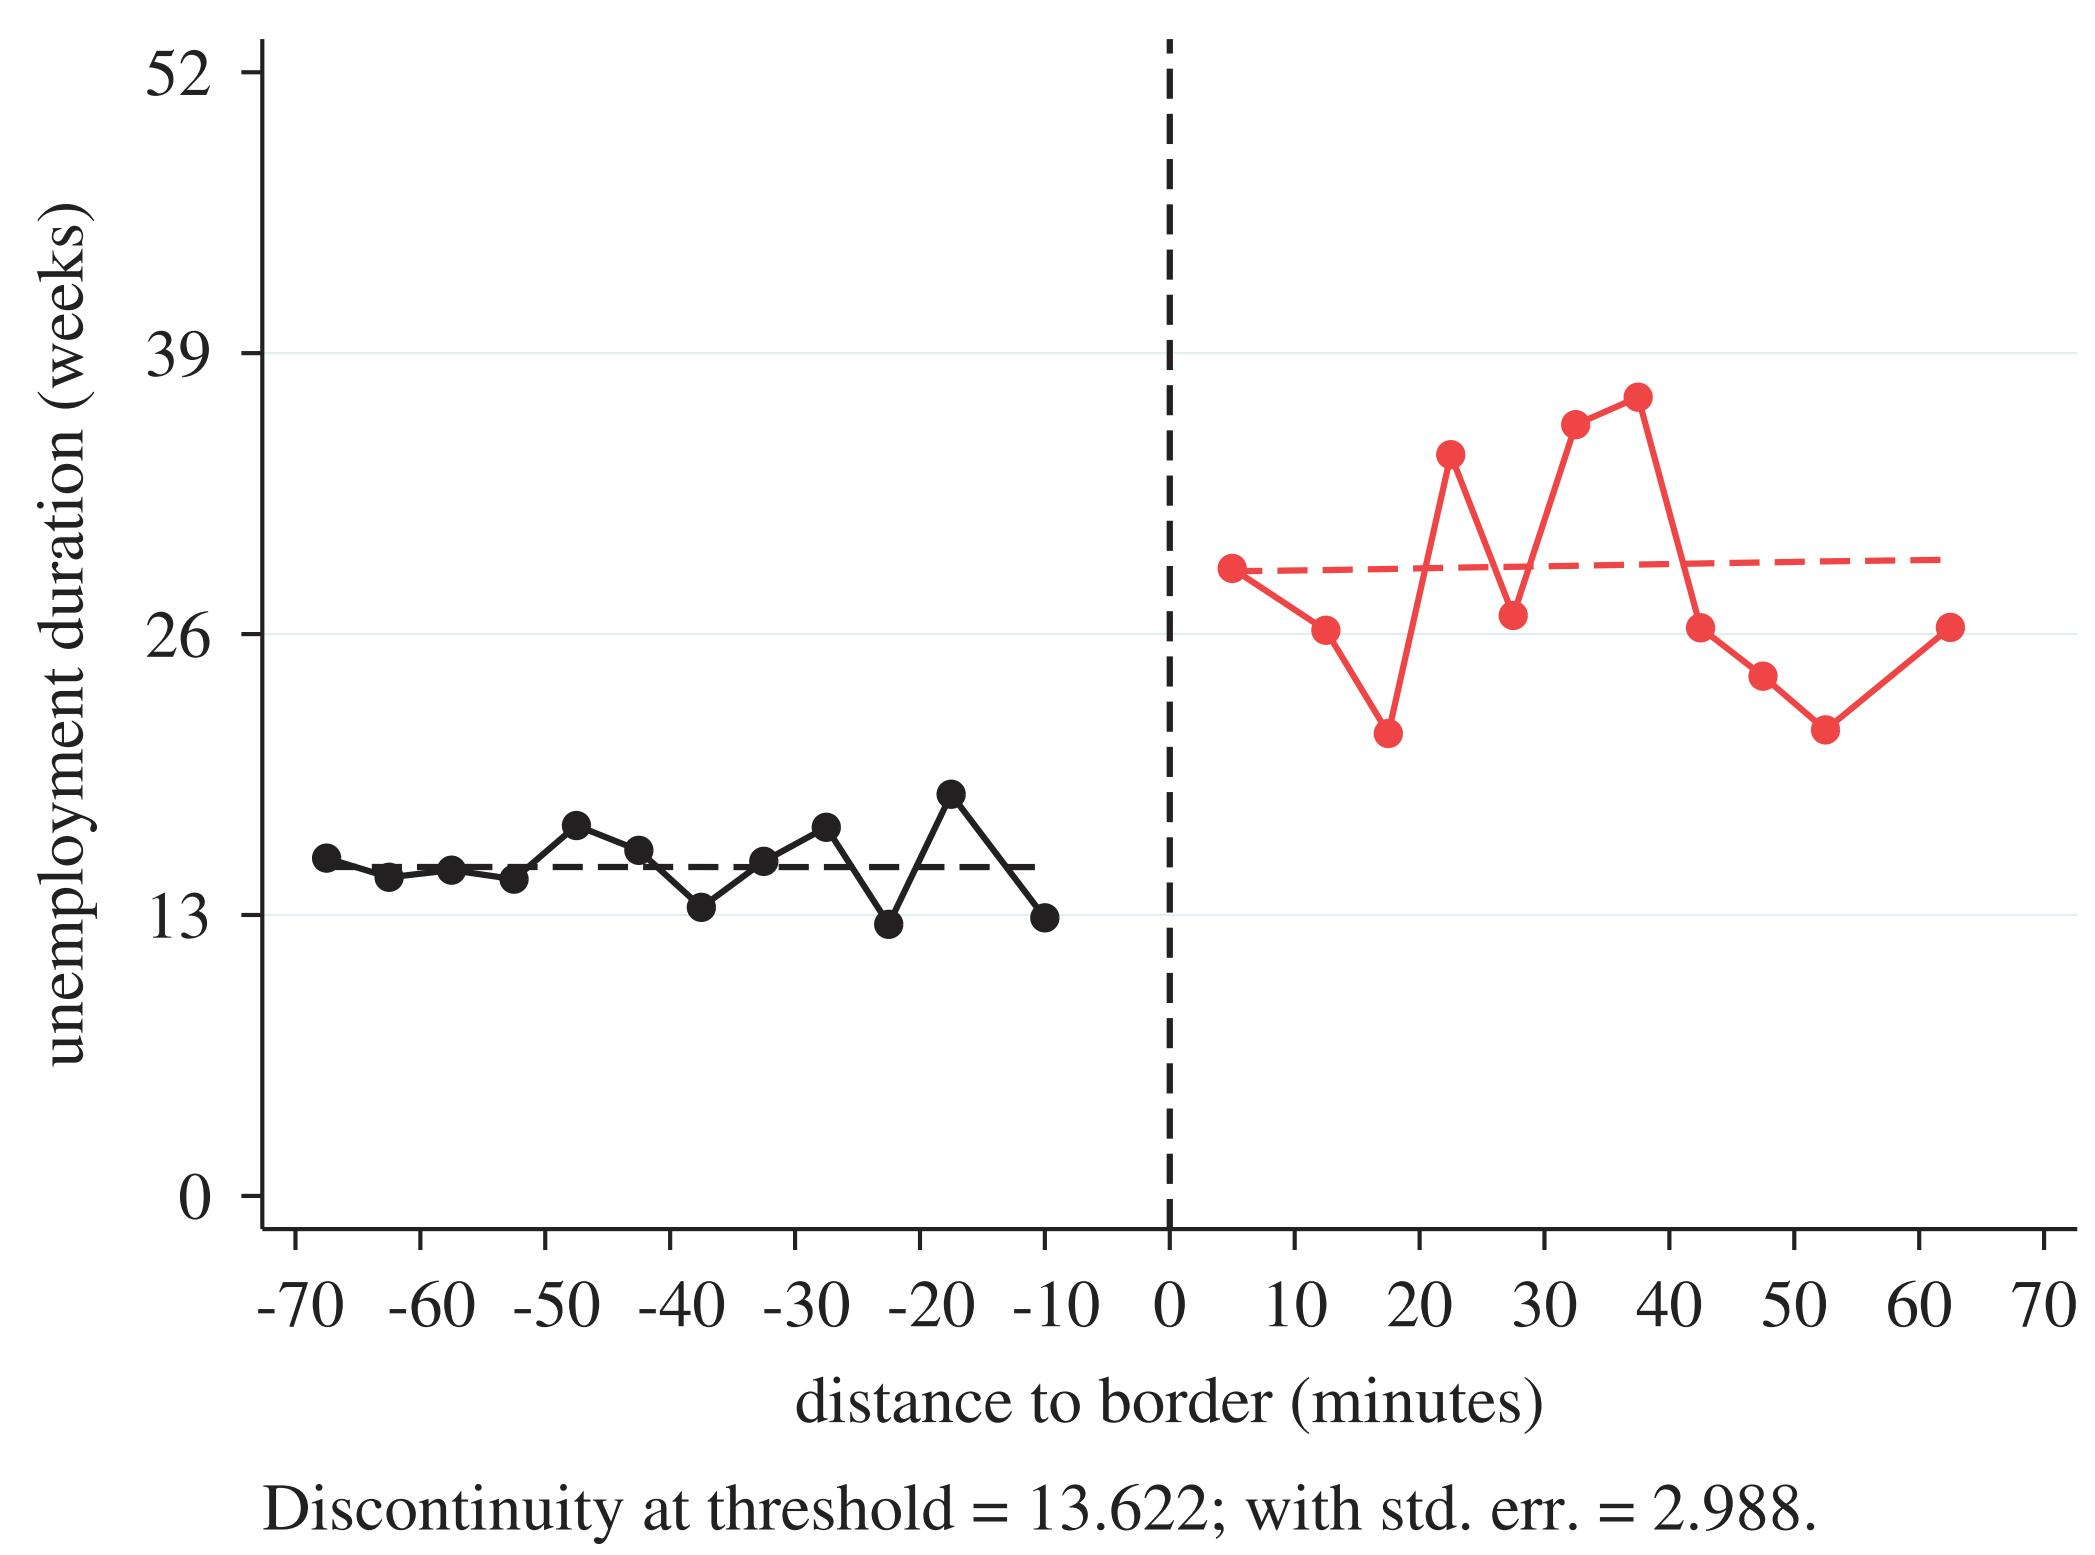
\includegraphics[width=.90\textwidth]{figure/srd_ui_f3.jpg}
	
\end{frame}



\begin{frame}{RDD Became Popular since late 1990s }{}
	
	\begin{itemize}
		\item The first RDD paper is Thistlethwaite and Campbell (1960), ``RD Analysis: An Alternative to Ex Post Fact
		Experiments," Journal of Education Psychology
		\vspace{0.2cm}
		\item RDD was not used much in economics until the late 1990s
		\vspace{0.2cm}
		\item But hundreds of studies since then, starting with Van der Klaauw (2002)
		\vspace{0.2cm}
		\item Two possible explanations:
		\vspace{0.2cm}
		\begin{itemize}
			\item Cutoff rules are very wide spread…
			\vspace{0.2cm}
			\item Much more data available now, especially administrative data sets
		\end{itemize}
		
	\end{itemize}
\end{frame}


\begin{frame}{RDD Became Popular since late 1990s }{}
	
	\begin{itemize}
		\item An important advantage of RD designs is that they are well suited to
		large administrative data sets with
		\vspace{0.2cm}
		\begin{itemize}
			\item Few covariates
			\vspace{0.2cm}
			\item Lots of observations and all the relevant information about cutoffs and assignment variables 
			\vspace{0.2cm}
			\item Since those have to be used in the administration of programs
		\end{itemize}
		
		
	\end{itemize}
\end{frame}





\title[]
{Identification}

\author{}
\institute{}
\date{}

\begin{frame}{}
    \titlepage
\end{frame}


%-------------------------------------------------------------
\begin{frame}{Sharp RDD and Fuzzy RDD}{}

\begin{itemize}
    \item Depending on whether the cutoff rule is perfectly enforced, RDD
          falls into two types:
    \vspace{0.25cm}
    \begin{itemize}
        \item[1] {\color{blue}Sharp RDD}: the probability of treatment
              \textbf{jumps from 0 to 1} at the cutoff
        \vspace{0.1cm}
        \begin{itemize}
            \item Everyone above the cutoff receives treatment;
                  no one below does
        \end{itemize}
        \vspace{0.2cm}
        \item[2] {\color{blue}Fuzzy RDD}: the probability of treatment
              \textbf{jumps discontinuously} at the cutoff,
              but the jump is less than 1
        \vspace{0.1cm}
        \begin{itemize}
            \item Not everyone follows the cutoff rule ---
                  some above the cutoff opt out;
                  some below manage to get in
        \end{itemize}
    \end{itemize}
    \vspace{0.2cm}
    \item Sharp RDD is a \textbf{special case} of fuzzy RDD
          where compliance is perfect
\end{itemize}
\end{frame}


%-------------------------------------------------------------
\begin{frame}{Fuzzy RDD}{Definition}

\begin{block}{Fuzzy RDD}
\begin{equation*}
    \lim_{\varepsilon\rightarrow 0}
    \Pr[D_i=1\mid A_i=c+\varepsilon]
    -
    \lim_{\varepsilon\rightarrow 0}
    \Pr[D_i=1\mid A_i=c-\varepsilon]
    \;\neq\; 0,\;1
\end{equation*}
\end{block}

\vspace{0.2cm}
\begin{itemize}
    \item The probability of treatment \textbf{jumps} at the cutoff,
          but the jump is \textbf{less than 1}

    \vspace{0.2cm}
    \item Crossing the cutoff \emph{shifts} the probability of treatment ---
          it does not \emph{determine} it
    \vspace{0.1cm}
    \begin{itemize}
        \item Example: scoring above a threshold makes one
              \emph{eligible} for a scholarship, but not everyone
              who is eligible actually uses it
    \end{itemize}

    \vspace{0.2cm}
    \item This is analogous to an \textbf{IV setting near the cutoff}:
          eligibility $Z_i = \mathbf{1}(A_i \geq c)$ shifts treatment
          $D_i$, but does not fully determine it
\end{itemize}
\end{frame}


%-------------------------------------------------------------
\begin{frame}{Treatment Probability and Assignment Variable}{Fuzzy RDD}
\begin{figure}
\begin{tikzpicture}[comment/.style={rectangle, text centered}]
    \centering
    \draw[very thick,->] (0,0) -- (6,0)
          node[anchor=north west] {$A$};
    \draw[very thick,->] (0,0) -- (0,4.2);

    \draw[very thick, blue] (3,4.2) -- (3,0)
          node[anchor=south, yshift=-0.7cm](3_0) {cutoff};
    \draw[very thick, blue] (0,0.7) -- (3,0.7)
          node[anchor=south, xshift=-1.2cm]
          {$\Pr[D_i=1]=0.15$};
    \draw[very thick, blue] (3,3.3) -- (6,3.3)
          node[anchor=north, xshift=-1.2cm]
          {$\Pr[D_i=1]=0.80$};

    \draw (0,0)  node[anchor=east] {$0$};
    \draw (0,4)  node[anchor=east] {$1$};

    \node[comment, above of=3_0, yshift=4.5cm]
          {Fuzzy Regression Discontinuity};
    \node[comment, left of=0_0, yshift=2.3cm, xshift=-0.5cm]
          {Probability of};
    \node[comment, left of=0_0, yshift=1.9cm, xshift=-0.5cm]
          {receiving treatment};
\end{tikzpicture}
\end{figure}
\end{frame}


%-------------------------------------------------------------
\begin{frame}{Sharp RDD}{Definition}

\begin{block}{Sharp RDD}
\begin{equation*}
    \lim_{\varepsilon\rightarrow 0}
    \Pr[D_i=1\mid A_i=c+\varepsilon]
    -
    \lim_{\varepsilon\rightarrow 0}
    \Pr[D_i=1\mid A_i=c-\varepsilon]
    \;=\; 1
\end{equation*}
\end{block}

\vspace{0.2cm}
\begin{itemize}
    \item Sharp RDD is a \textbf{special case} of fuzzy RDD
    \vspace{0.2cm}
    \item The jump in treatment probability is exactly 1:
    \vspace{0.1cm}
    \begin{itemize}
        \item Nobody below the cutoff receives treatment;
              everybody above the cutoff does
        \vspace{0.1cm}
        \item The assignment rule is perfectly enforced ---
              \textbf{all} individuals are compliers
    \end{itemize}
    \vspace{0.2cm}
    \item Treatment eligibility $Z_i$ and actual treatment $D_i$
          coincide: $Z_i = D_i$
\end{itemize}
\end{frame}


%-------------------------------------------------------------
\begin{frame}{Treatment Probability and Assignment Variable}{Sharp RDD}
\begin{figure}
\begin{tikzpicture}[comment/.style={rectangle, text centered}]
    \centering
    \draw[very thick,->] (0,0) -- (6,0)
          node[anchor=north west] {$A$};
    \draw[very thick,->] (0,0) -- (0,4.2);

    \draw[very thick, blue] (3,4.2) -- (3,0)
          node[anchor=south, yshift=-0.7cm](3_0) {cutoff};
    \draw[very thick, blue] (0,0) -- (3,0)
          node[anchor=south, xshift=-1.2cm]
          {$\Pr[D_i=1]=0$};
    \draw[very thick, blue] (3,4) -- (6,4)
          node[anchor=north, xshift=-1.2cm]
          {$\Pr[D_i=1]=1$};

    \draw (0,0)  node[anchor=east] {$0$};
    \draw (0,4)  node[anchor=east] {$1$};

    \node[comment, above of=3_0, yshift=4.5cm]
          {Sharp Regression Discontinuity};
    \node[comment, left of=0_0, yshift=2.3cm, xshift=-0.5cm]
          {Probability of};
    \node[comment, left of=0_0, yshift=1.9cm, xshift=-0.5cm]
          {receiving treatment};
\end{tikzpicture}
\end{figure}
\end{frame}


%-------------------------------------------------------------
\begin{frame}{Potential Outcomes Framework}{Why Do We Need It?}

\begin{itemize}
    \item In \textbf{sharp} RDD, eligibility $Z_i$ perfectly determines
          treatment $D_i$, so estimating the effect of crossing the cutoff
          is enough
    \vspace{0.3cm}
    \item In \textbf{fuzzy} RDD, $Z_i$ only \emph{shifts} $D_i$ ---
          we need to formally distinguish:
    \vspace{0.15cm}
    \begin{itemize}
        \item $Z_i$: \textbf{treatment eligibility}
              (determined by the cutoff rule)
        \vspace{0.1cm}
        \item $D_i$: \textbf{treatment received}
              (the individual's actual choice)
    \end{itemize}
    \vspace{0.3cm}
    \item This $Z_i \to D_i$ structure is exactly the
          \textbf{IV framework}:
    \vspace{0.15cm}
    \begin{center}
    \small
    \begin{tabular}{ccccc}
        Instrument & & Endogenous variable & & Outcome \\
        $Z_i$ & $\longrightarrow$ & $D_i$ & $\longrightarrow$ & $Y_i$
    \end{tabular}
    \end{center}
\end{itemize}
\end{frame}


%-------------------------------------------------------------
\begin{frame}{Potential Outcomes Framework}{Eligibility and Potential Treatments}

\begin{itemize}

    \item \textcolor{blue}{Treatment Eligibility}
    \begin{align*}
        Z_{i}=\begin{cases}
            1 & \text{if } A_i\geq c \quad \text{(above cutoff, eligible)}\\
            0 & \text{if } A_i < c  \quad \text{(below cutoff, not eligible)}
        \end{cases}
    \end{align*}

    \vspace{0.2cm}
    \item \textcolor{blue}{Potential Treatments} \;
          $D^z_i$: treatment status given eligibility $Z_i = z$
    \vspace{0.1cm}
    \begin{itemize}
        \item $D^{1}_i$: would individual $i$ get treatment
              \emph{if} eligible? ($Z_i=1$)
        \vspace{0.1cm}
        \item $D^{0}_i$: would individual $i$ get treatment
              \emph{if} not eligible? ($Z_i=0$)
    \end{itemize}

    \vspace{0.2cm}
    \item \textcolor{blue}{Observed Treatment}
    \begin{equation*}
        D_{i} = Z_{i}D^{1}_{i} + (1-Z_{i})D^{0}_{i}
    \end{equation*}

\end{itemize}
\end{frame}


%-------------------------------------------------------------
% \begin{frame}{Compliance Types}{Fuzzy RDD}

% \begin{itemize}
%     \item Based on $(D^1_i,\, D^0_i)$, we can classify individuals
%           into \textbf{four compliance types}:
%     \vspace{0.15cm}
% \end{itemize}

% \begin{center}
% \small
% \begin{tabular}{llcc}
%     \toprule
%     Type & Description & $D^1_i$ & $D^0_i$ \\
%     \midrule
%     \textbf{Compliers}    & Take treatment iff eligible   & 1 & 0 \\
%     Always-takers         & Always take treatment         & 1 & 1 \\
%     Never-takers          & Never take treatment          & 0 & 0 \\
%     Defiers               & Take treatment iff \emph{not} eligible & 0 & 1 \\
%     \bottomrule
% \end{tabular}
% \end{center}

% \vspace{0.2cm}
% \begin{itemize}
%     \item In \textbf{sharp} RDD: everyone is a \textbf{complier}
%           ($D^1_i=1$, $D^0_i=0$ for all $i$)
%     \vspace{0.15cm}
%     \item In \textbf{fuzzy} RDD: there are always-takers and never-takers
%           in addition to compliers
%     \vspace{0.15cm}
%     \item Assuming \textbf{no defiers} (monotonicity), the fuzzy RDD
%           estimate identifies the average treatment effect for
%           \textbf{compliers} near the cutoff
% \end{itemize}
% \end{frame}


%-------------------------------------------------------------
\begin{frame}{Using the Cutoff as an Instrument}{}

\begin{itemize}
    \item The jump in \textbf{outcomes} at the cutoff is the
          \textbf{reduced form} (Intent-to-Treat, ITT) ---
          the effect of \emph{eligibility} $Z_i$:
    \begin{equation*}
        \underbrace{
        \lim_{\varepsilon\rightarrow 0}
        \mathrm{E}[Y_{i}\mid A_{i}=c+\varepsilon]
        -
        \lim_{\varepsilon\rightarrow 0}
        \mathrm{E}[Y_{i}\mid A_{i}=c-\varepsilon]
        }_{\text{Reduced form (ITT): effect of crossing the cutoff}}
    \end{equation*}

    \vspace{0.15cm}
    \item The jump in \textbf{treatment probability} is the
          \textbf{first stage}:
    \begin{equation*}
        \underbrace{
        \lim_{\varepsilon\rightarrow 0}
        \mathrm{E}[D_{i}\mid A_{i}=c+\varepsilon]
        -
        \lim_{\varepsilon\rightarrow 0}
        \mathrm{E}[D_{i}\mid A_{i}=c-\varepsilon]
        }_{\text{First stage: jump in treatment take-up}}
    \end{equation*}

    \vspace{0.15cm}
    \item To recover the effect of \textbf{treatment received} $D_i$:
          divide the reduced form by the first stage
\end{itemize}
\end{frame}


%-------------------------------------------------------------
\begin{frame}{Fuzzy RDD as IV}{Wald Estimator}

\begin{itemize}
    \item The fuzzy RDD estimator is a \textbf{Wald estimate} at cutoff $c$:
    \begin{equation*}
        \alpha_{FRD}
        =
        \frac{
          \displaystyle
          \lim_{\varepsilon\rightarrow 0}
          \mathrm{E}[Y_{i}\mid A_{i}=c+\varepsilon]
          -
          \lim_{\varepsilon\rightarrow 0}
          \mathrm{E}[Y_{i}\mid A_{i}=c-\varepsilon]
        }{
          \displaystyle
          \lim_{\varepsilon\rightarrow 0}
          \mathrm{E}[D_{i}\mid A_{i}=c+\varepsilon]
          -
          \lim_{\varepsilon\rightarrow 0}
          \mathrm{E}[D_{i}\mid A_{i}=c-\varepsilon]
        }
        =
        \frac{\text{ITT}}{\text{First stage}}
    \end{equation*}

    % \vspace{0.2cm}
    % \item $\alpha_{FRD}$ is a \textbf{Local Average Treatment Effect (LATE)}:
    %       the average treatment effect for \textbf{compliers near the cutoff}
    % \vspace{0.1cm}
    % \begin{itemize}
    %     \item Example: the effect of actually attending NTU for students who
    %           would enroll \emph{only if} their test score is above the threshold
    % \end{itemize}

    % \vspace{0.2cm}
    % \item For $Z_i = \mathbf{1}(A_i \geq c)$ to be a valid instrument,
    %       we need:
    % \vspace{0.1cm}
    % \begin{itemize}
    %     \item \textbf{Relevance}: crossing the cutoff raises $\Pr(D_i=1)$
    %           (first stage $\neq 0$)
    %     \vspace{0.1cm}
    %     \item \textbf{Exclusion}: crossing the cutoff affects $Y_i$ only
    %           through $D_i$
    %     \vspace{0.1cm}
    %     \item \textbf{Monotonicity}: no defiers
    % \end{itemize}
\end{itemize}
\end{frame}







\begin{frame}{Identification Assumptions}{Fuzzy RDD}

\begin{itemize}
  \item \textbf{Continuity}: potential outcomes and potential treatment status would change smoothly at the cutoff without the eligibility rule.

  \vspace{0.2cm}

  \item \textbf{First stage}: treatment probability changes discontinuously at the cutoff:
  \[
    \lim_{\varepsilon\rightarrow 0}\mathrm{E}[D_i\mid A_i=c+\varepsilon]
    \neq
    \lim_{\varepsilon\rightarrow 0}\mathrm{E}[D_i\mid A_i=c-\varepsilon].
  \]

  \vspace{0.2cm}

  \item \textbf{Monotonicity}: crossing the cutoff does not make some individuals less likely to receive treatment:
  \[
    D_i^1 \geq D_i^0.
  \]

  \vspace{0.2cm}

  \item \textbf{Exclusion restriction}: eligibility affects outcomes only through actual treatment.
\end{itemize}

\end{frame}





\begin{frame}{Fuzzy RDD and Compliers}
	\begin{itemize}
		
		\item We can define four types of individuals based on whether they fellow the treatment assignment:
		\vspace{0.2cm}
		\begin{itemize}
			\vspace{0.3cm}
			\item \textbf{Compliers}: $\mathrm{D}^{1}_{i}>\mathrm{D}^{0}_{i}$ ($\mathrm{D}^{0}_{i}=0$ and $\mathrm{D}^{1}_{i}=1$)
			\begin{itemize}
				\item David's test score is above NTU cutoff and enrolled in NTU 
				\vspace{0.2cm}
				\item David's test score is below NTU cutoff and did not enroll in NTU 
			\end{itemize}
			\item \textbf{Always-takers}: $\mathrm{D}^{1}_{i}=\mathrm{D}^{0}_{i}=1$
			\begin{itemize}
				\item John always can enroll in NTU (whether or not his test score is above NTU cutoff)
				\vspace{0.2cm}
			\end{itemize}			
			\item \textbf{Never-takers}: $\mathrm{D}^{1}_{i}=\mathrm{D}^{0}_{i}=0$
			\begin{itemize}
				\item Hank never enroll in NTU (whether or not his test score is above NTU cutoff)
				\vspace{0.2cm}
			\end{itemize}			
			\item \textbf{Defiers}: $\mathrm{D}^{1}_{i}<\mathrm{D}^{0}_{i}$ ($\mathrm{D}^{0}_{i}=1$ and $\mathrm{D}^{1}_{i}=0$)
			\begin{itemize}
				\item Jimmy's test score is above NTU cutoff and did NOT enroll in NTU  
				\vspace{0.2cm}
				\item Jimmy's test score is below NTU cutoff but enrolled in NTU  
			\end{itemize}
			
			
		\end{itemize}
		
	\end{itemize}
\end{frame}




\begin{frame}{Fuzzy RDD and Compliers}{}
	
	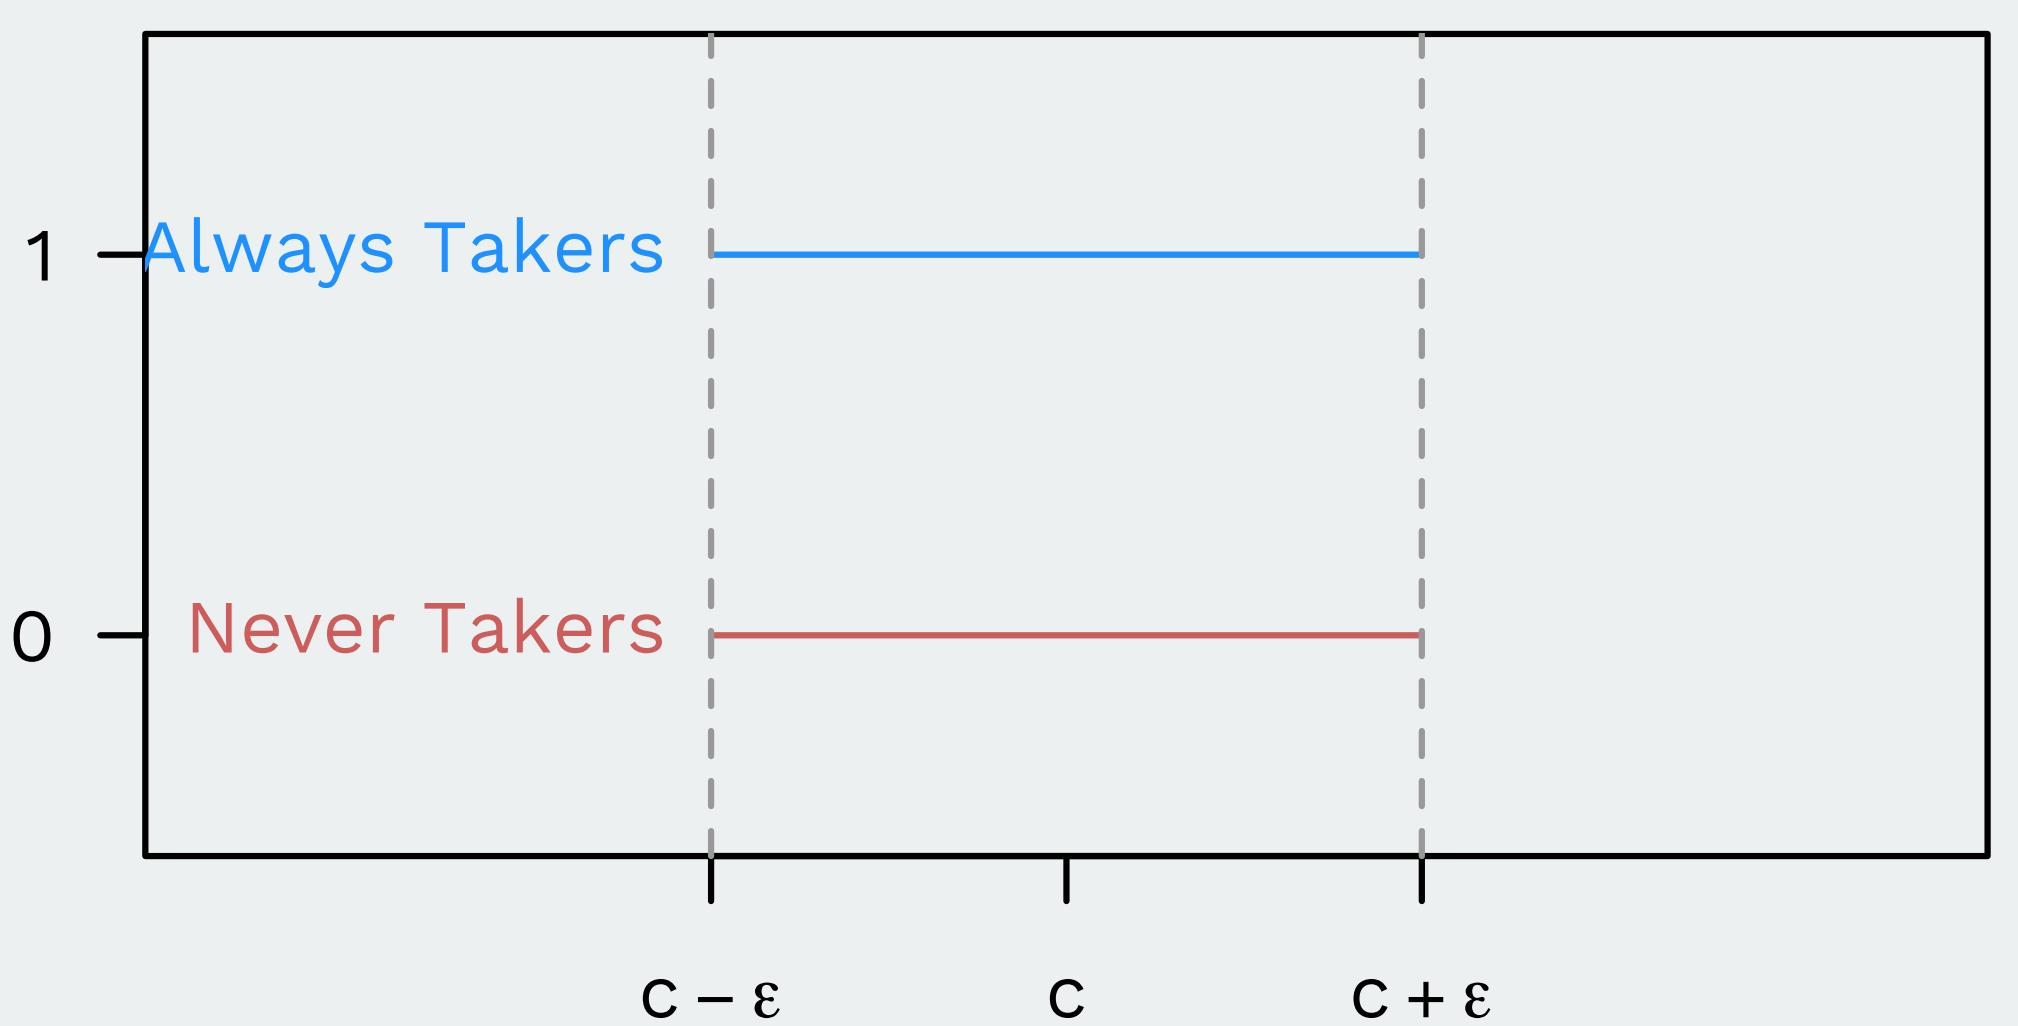
\includegraphics[width=1.0\textwidth]{figure/complier_f1.jpg}
	
	
\end{frame}


\begin{frame}{Fuzzy RDD and Compliers}{}
	
	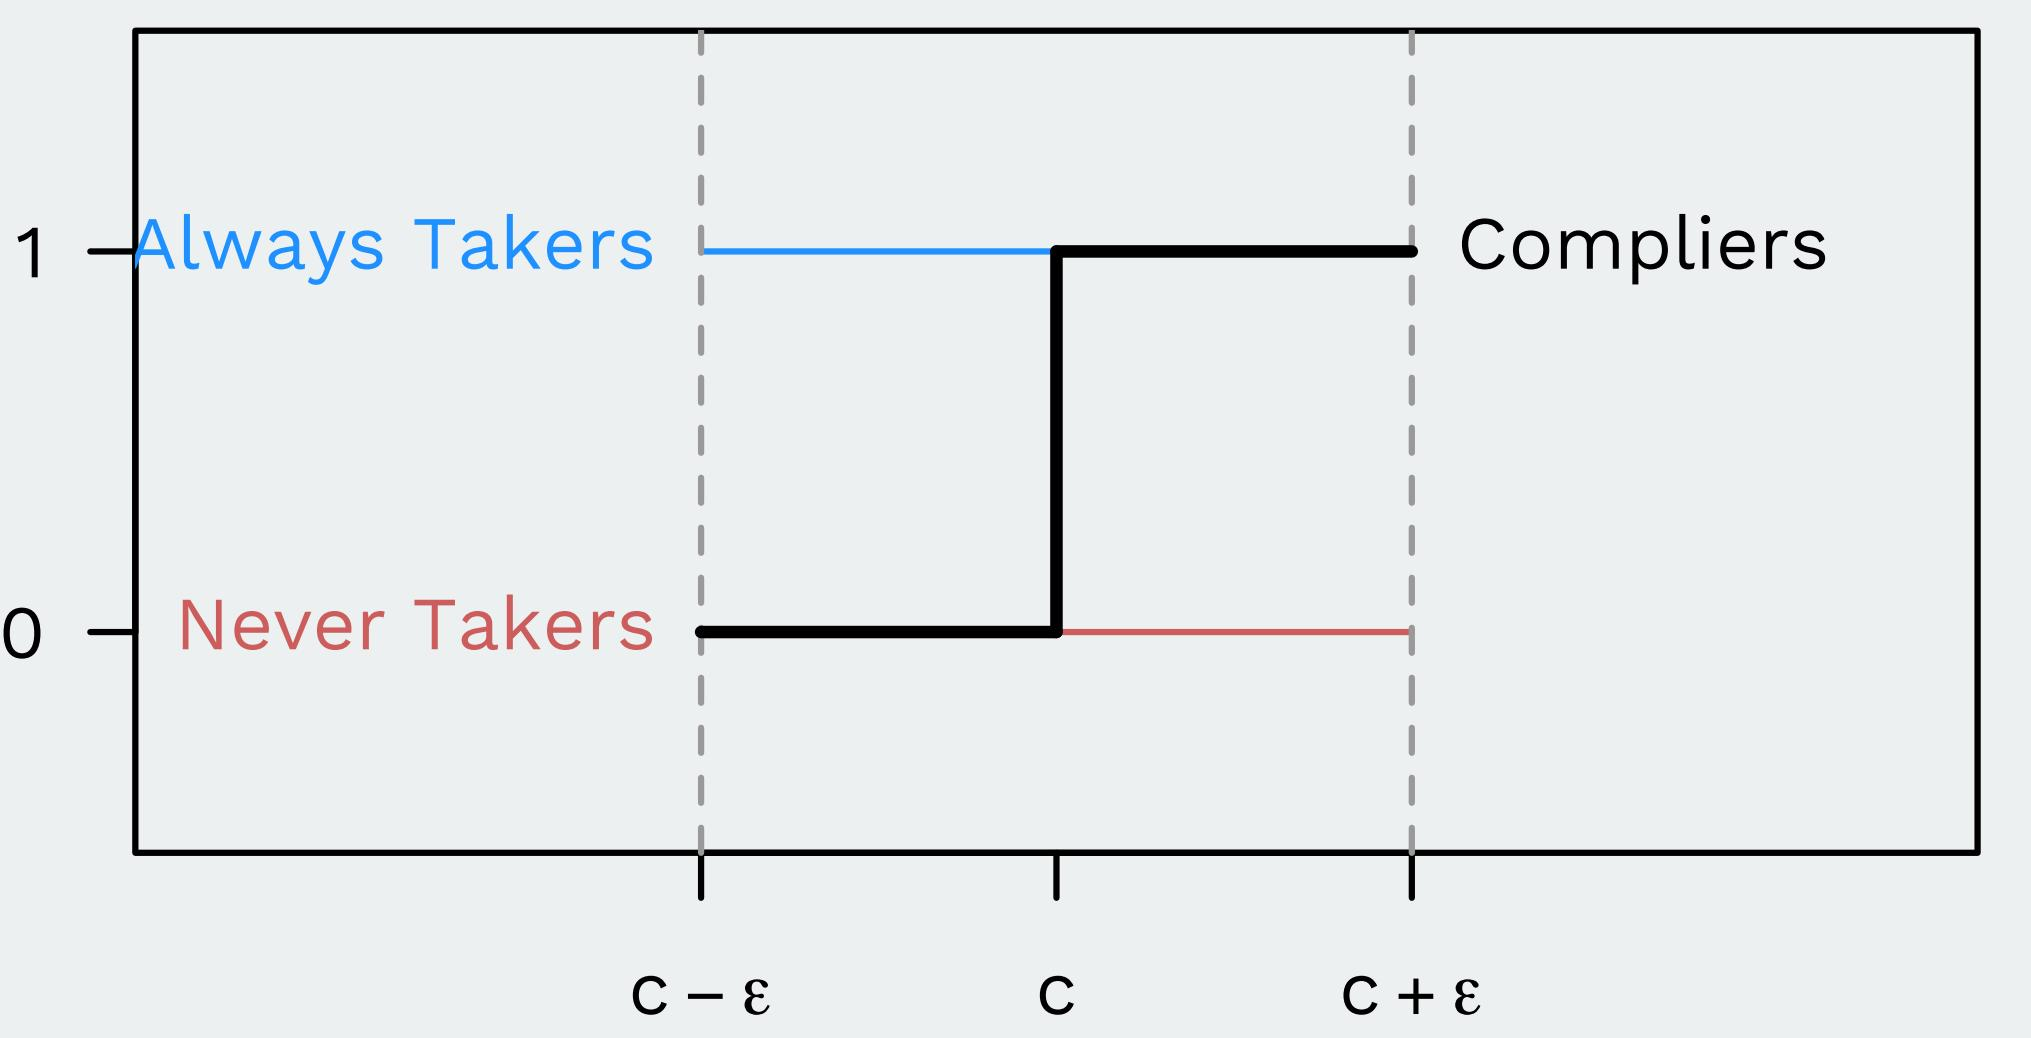
\includegraphics[width=1.0\textwidth]{figure/complier_f2.jpg}
	
	
\end{frame}

\begin{frame}{Identification Results for Fuzzy RDD}
	\begin{itemize}
		
		\begin{block}{Fuzzy RDD Identify LATE at cutoff c}
			\begin{equation*}
				\begin{aligned}
					\alpha_{FRD} &=\dfrac{\lim_{\varepsilon\rightarrow 0}\mathrm{E}[Y_{i}|A_{i}=x+\varepsilon]-\lim_{\varepsilon\rightarrow 0}\mathrm{E}[Y_{i}|A_{i}=x-\varepsilon]}{\lim_{\varepsilon\rightarrow 0}\mathrm{E}[D_{i}|A_{i}=x+\varepsilon]-\lim_{\varepsilon\rightarrow 0}\mathrm{E}[D_{i}|A_{i}=x-\varepsilon]}  \\
					&= \mathrm{E}[ \mathrm{Y}^{1}_{i} - \mathrm{Y}^{0}_{i} | \mathrm{D}^{1}_{i} > \mathrm{D}^{0}_{i}, A_{i}=c]
				\end{aligned}
			\end{equation*} 
		\end{block}
		
		
		\item The estimate in fuzzy RDD represents the \textbf{causal effect for compliers} (local average treatment effect, LATE) at cutoff $c$
		\vspace{0.2cm}
		\item \textbf{Compliers} are those who receive the
		treatment when they follow treatment eligibility rule 
		($A_i\geq c$), but would not otherwise receive it ($A_i< c$)	
		%\item Lottery IV can identify the causal effect of military service on lifetime earnings for those who obey the lottery results (e.g. David and Tim)
	\end{itemize}
\end{frame}



\title[]
{Examine Validity of Identification Assumptions}

\author
{}

\institute{}

\date
{}

\begin{frame}{}
	\titlepage
\end{frame}






\begin{frame}{Test Internal Validity of RDD}{Examine ``Discontinuity" in Nonoutcome Variables}
	
	\textbf{1. Examine ``Discontinuity" in Nonoutcome Variables}
	
	\begin{itemize}
		\vspace{0.2cm}	
		\item Construct a similar graph to the one before but using a covariate as the ``outcome"
		\vspace{0.2cm}	
		\item There should be \textbf{NO jump in other covariates}
		\vspace{0.2cm}	
		\item If the covariates would jump at the cutoff one would doubt the identifying assumption
		
	\end{itemize}
\end{frame}




\begin{frame}{Test Internal Validity of RDD}{Sorting Behavior}
	
	\textbf{2. Examine ``Discontinuity" in Density of the assignment variable}
	
	\begin{itemize}
		\vspace{0.2cm}	
		\item Individuals may invalidate the \textbf{continuity assumption} if they strategically manipulate assignment variable $A$ to be just above or below the cutoff
		\vspace{0.2cm}
		\item That is, people just above and just below the cutoff are no longer comparable
		\vspace{0.2cm}
		
		
	\end{itemize}
\end{frame}



\begin{frame}{Consequence of Sorting Behavior}{Example}
	
	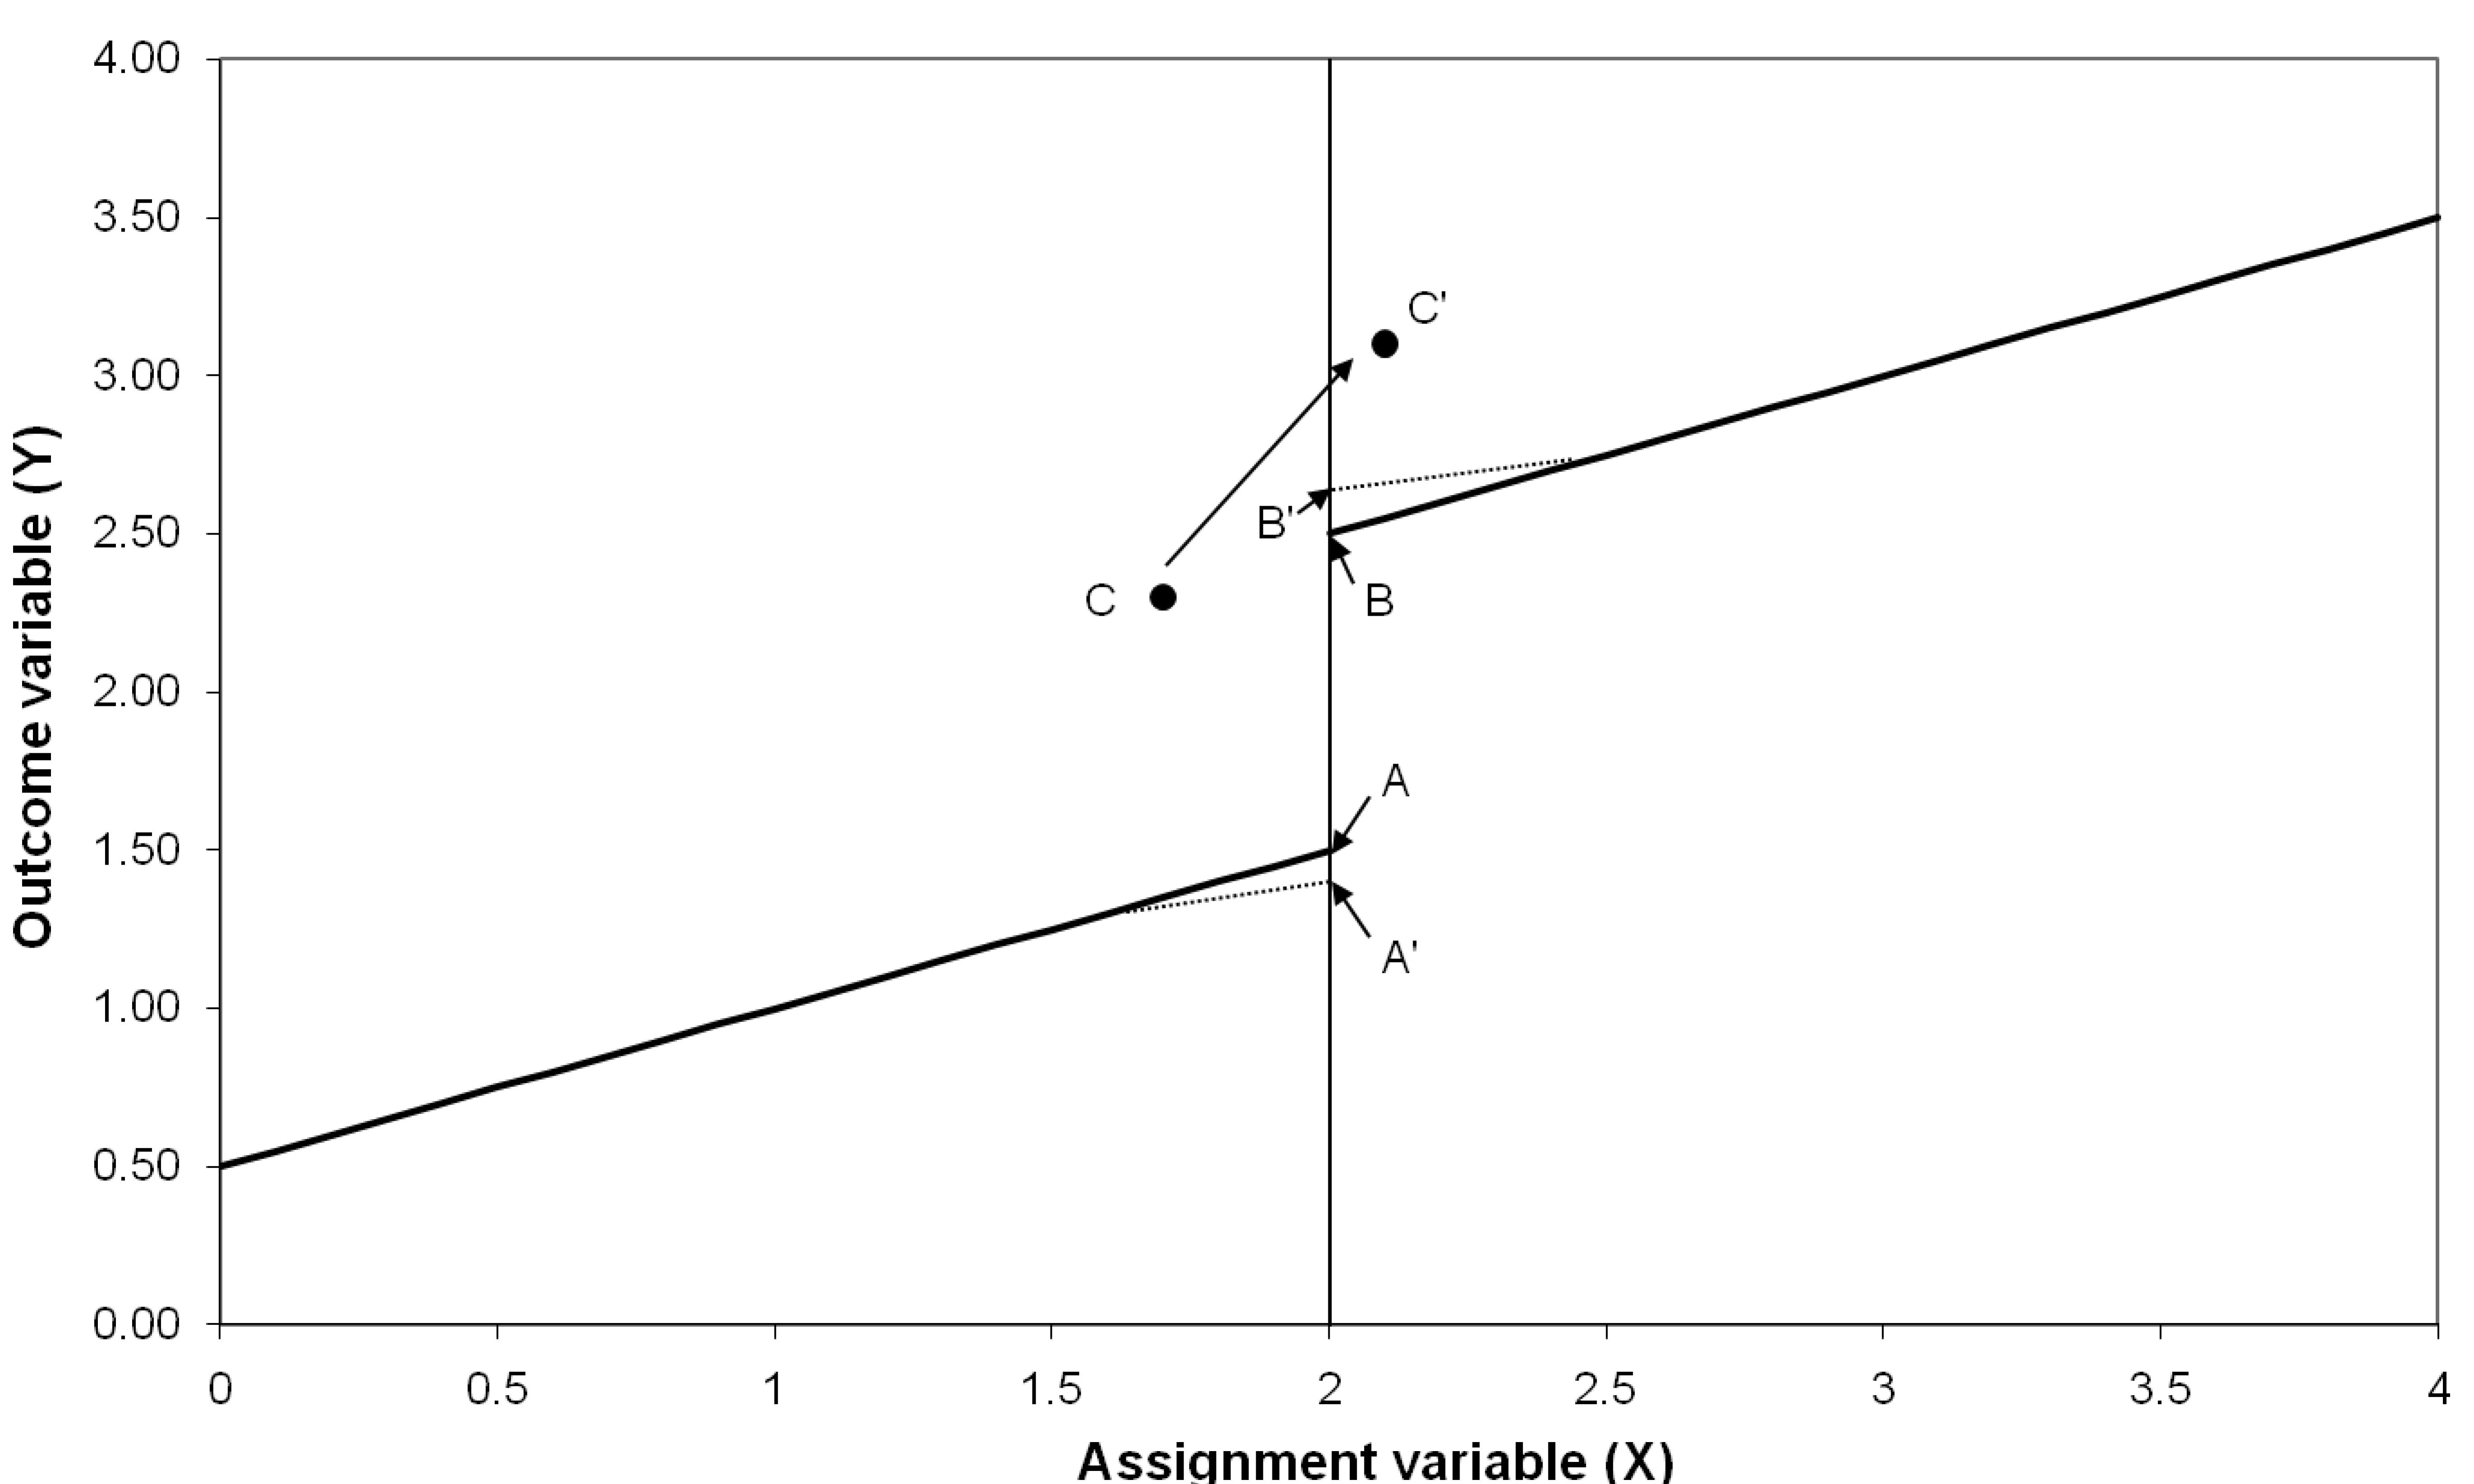
\includegraphics[width=1.0\textwidth]{figure/manu_f1.jpg}
	
	
\end{frame}



\begin{frame}{Sorting Behavior}{Example}
	\begin{itemize}
		
		\item This is a concern especially if the exact value of the cutoff is known to the individuals in advance
		\vspace{0.2cm}
			\begin{itemize}
		\item Such sorting behavior may create a \textbf{discontinuity in the distribution of $A$ at the cutoff}
		\vspace{0.2cm}
		\item That is, ``bunching" to the right or to the left of the cutoff
			\end{itemize}
	\end{itemize}
	
\end{frame}




\begin{frame}{Sorting Behavior}{Example}
	
	Adriana Camacho and Emily Conover (2011) ``\textbf{Manipulation of Social Program Eligibility}" AEJ: Economic Policy
			\vspace{0.2cm}
	\begin{itemize}
		\item Manipulation of a poverty index in Colombia
		\vspace{0.2cm}
			\begin{itemize}
		\item A poverty index is used to decide eligibility for social programs 
		\vspace{0.2cm}
			\end{itemize}
		\item The algorithm to create the poverty index \textbf{becomes public} during the second half of 1997
	\end{itemize}
\end{frame}




\begin{frame}{Sorting Behavior}{Example}
	
	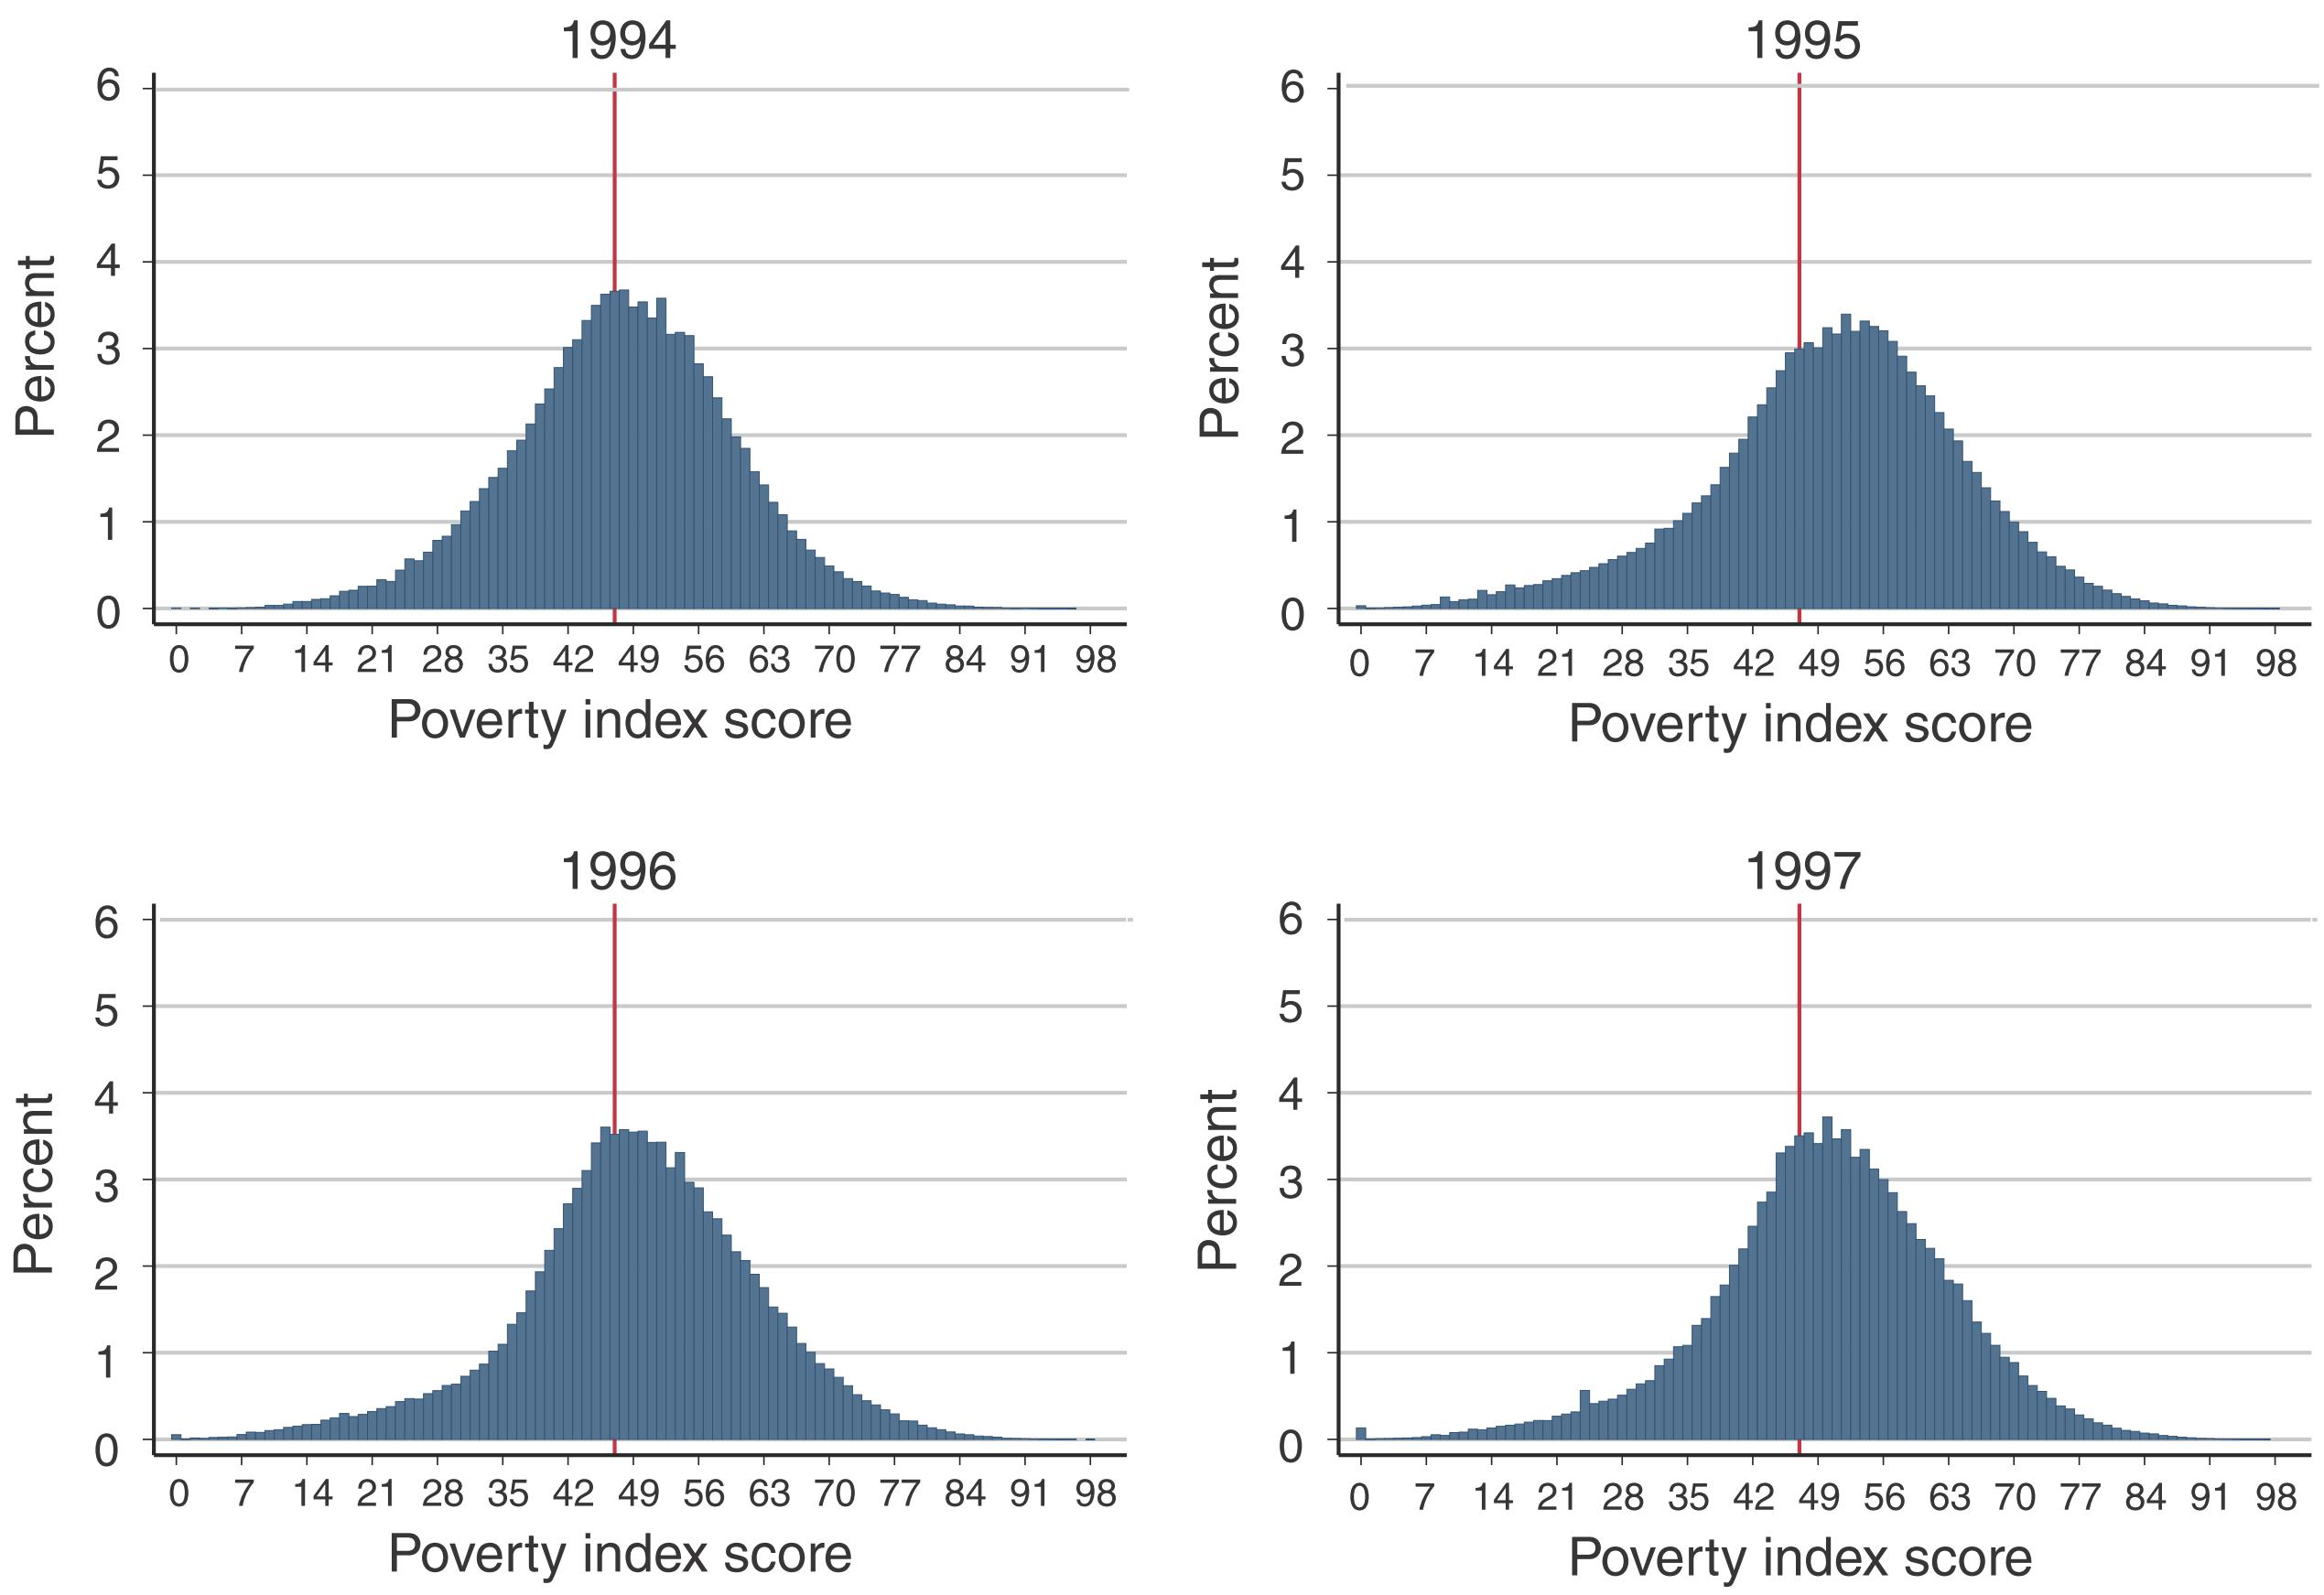
\includegraphics[width=0.9\textwidth]{figure/RD_density_f1.jpg}
	
	
\end{frame}



\begin{frame}{Sorting Behavior}{Example}
	
	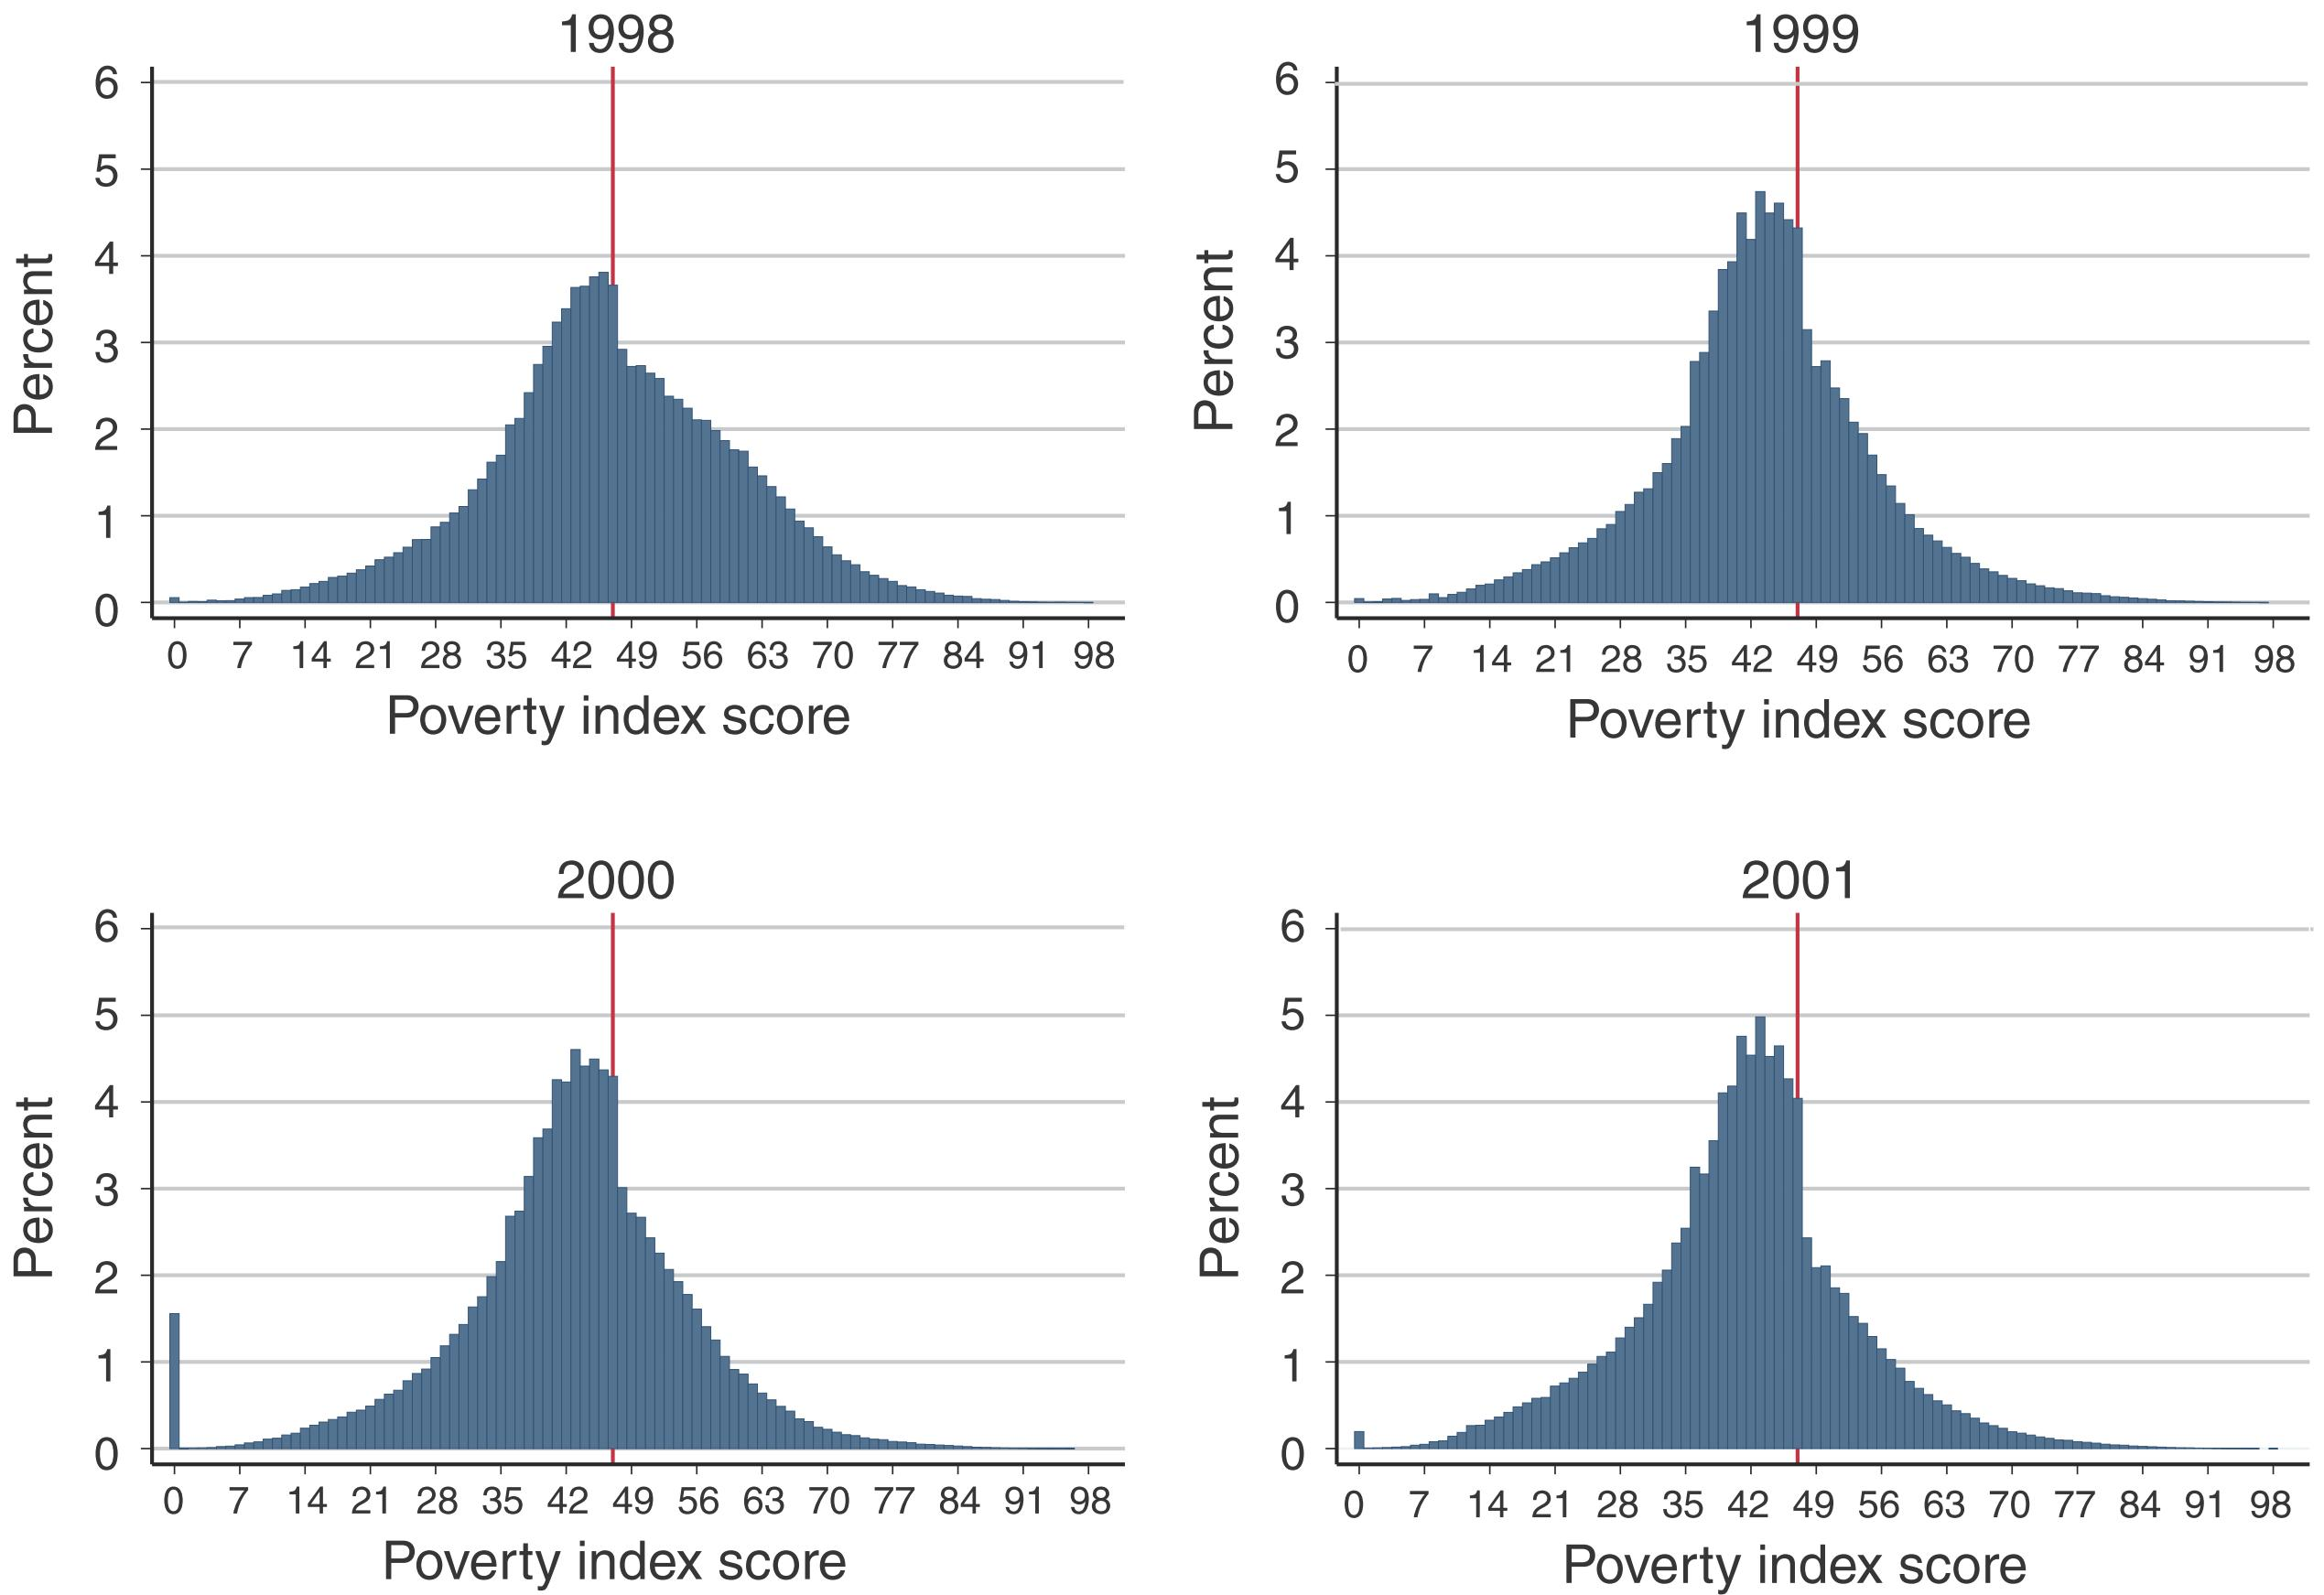
\includegraphics[width=0.9\textwidth]{figure/RD_density_f2.jpg}
	
	
\end{frame}



\begin{frame}{Test Internal Validity of RDD}{Examine Discontinuity in Density of the Assignment Variable}
	
	\textbf{How to Examine ``Discontinuity" in Density of the assignment variable}
	
	\begin{itemize}
		\vspace{0.2cm}	
		\item Plot the number of observations in each bin of assignment variable
		\vspace{0.1cm}	
		\item Investigate whether there is a \textbf{discontinuity in the distribution of the assignment variable} at the threshold
		\vspace{0.2cm}	
			\begin{itemize}
		\item A discontinuity in the density suggests that people might manipulate the assignment variable around the threshold
			\end{itemize}
		
	\end{itemize}
\end{frame}







%\begin{frame}{Test Internal Validity of RDD}{Formal Test for Density Discontinuity (McCrary Test)} % More specific title
%	
%	\begin{itemize}
%		\item A formal statistical test for discontinuity in the density of the assignment variable was proposed by \textbf{McCrary (2008, Journal of Econometrics)}.
%		\vspace{0.3cm}
%		\item \textbf{Key Steps of the McCrary Test}:
%		\vspace{0.1cm}
%		\begin{itemize}
%			\item[1.] \textbf{Binning}: Partition the assignment variable ($A$) into discrete bins. Calculate the number of observations (frequency, $N_j$) for each bin $j$.
%			\vspace{0.2cm}
%			\item[2.] \textbf{Centering}: Ensure that no bin straddles or overlaps the cutoff point $c$. The running variable for the local regressions will be the midpoint of each bin ($x_j$).
%			\vspace{0.2cm}
%			\item[3.] \textbf{Local Linear Regressions}: Run local linear regressions using the bin frequencies ($N_j$) as the outcome variable and bin midpoints ($x_j$) as the covariate. This is done separately for data to the left and to the right of the cutoff $c$.
%			% Y_bin = N_j (frequency counts)
%			% X_bin = x_j (bin midpoints)
%			\vspace{0.2cm}
%			\item[4.] \textbf{Test Statistic ($\theta$)}: The test statistic is the estimated log difference in the heights of the (smoothed) density at the cutoff. This is derived from the difference in the intercepts of the two local linear regressions at $c$.
%			% theta = log(f_R(c)) - log(f_L(c))
%			\vspace{0.2cm}
%			\item[5.] \textbf{Inference}: A statistically significant $\theta \neq 0$ provides evidence of a discontinuity in the density, suggesting potential manipulation of the assignment variable.
%		\end{itemize}
%	\end{itemize}
%\end{frame}









\begin{frame}{Test Internal Validity of RDD}{Examine Density of the assignment variable}
	
	%\textbf{2. Examine ``Discontinuity" in Density of the assignment variable}
	
	\begin{itemize}
		\vspace{0.2cm}	
		\item A formal test is provided by McCrary (2008)
		\vspace{0.2cm}		
		\begin{itemize}
			\item[1] Partition the assignment variable into bins and calculate frequencies (number of observations) in each bins
			\vspace{0.2cm}
			\item[2] Calculate frequencies (number of observations) in each bin	 
			\vspace{0.2cm}
			\item[3] Ensure that no bin overlaps the cutoff
			\vspace{0.2cm}
			\item[4] \textbf{Run two local linear regressions}, one to the right and one to the left of the cutoff
			\vspace{0.2cm}
			\item[5] In these regressions,  the bin midpoints
			are the regressors and \textbf{number of observations is outcome}
			\vspace{0.2cm}
			\item[6] Test whether log difference of the intercepts of the two regressions
			is statistically different from zero	
			
			
		\end{itemize}
		
		%\item A discontinuity in the density suggests that there is some manipulation of R around the threshold going on
		% \vspace{0.2cm}	
		%\item In the first step you partition the assignment variable into bins and calculate frequencies (number of observations) in the bins
		% \vspace{0.2cm}	
		%\item In the second step you treat those frequency counts as dependent variable in a local linear regression as before
		
		
	\end{itemize}
\end{frame}



\title[]
{Estimation}

\author
{}

\institute{}

\date
{}

\begin{frame}{}
	\titlepage
\end{frame}



\begin{frame}{RDD Estimation}{Overview}
	\begin{itemize}
		
		\item There are two strategies for getting RD estimates:
		\begin{itemize}
			\vspace{0.2cm}
			\item[1] Parametric/global method:
			\vspace{0.2cm}  
			\begin{itemize}
				\item Use all available observations
				\vspace{0.2cm}
				\item Estimate treatment effects based on a \textbf{specific functional form} for the outcome and assignment variable relationship
								\vspace{0.2cm}
			\end{itemize}
				\item[2] Nonparametric/local method:
			\vspace{0.2cm} 
			\begin{itemize}
				\item Use the observations around cutoff
				\vspace{0.2cm}
				\item Compare the outcome of treated and untreated observations that lie \textbf{within specific bandwidth}
			\end{itemize}
			
		\end{itemize}
		
	\end{itemize}
\end{frame}



% \begin{frame}{Fuzzy RDD Estimation}{Overview}
% 	\begin{itemize}
% 		\item Two strategies for estimating the fuzzy RDD treatment effect (LATE):
% 		\vspace{0.2cm}
% 		\begin{itemize}
% 			\item[1] \textbf{Parametric/Global} method:
% 			\vspace{0.2cm}
% 			\begin{itemize}
% 				\item Use all available observations
% 				\item Control for $\mathrm{f}(A_i)$ via a polynomial
% 				\item Estimate via 2SLS (instrument $D_i$ with $Z_i$)
% 				\vspace{0.2cm}
% 			\end{itemize}
% 			\item[2] \textbf{Nonparametric/Local} method:
% 			\vspace{0.2cm}
% 			\begin{itemize}
% 				\item Use only observations close to the cutoff (within bandwidth $h$)
% 				\item No global functional form assumed
% 				\item \texttt{rdrobust} with \texttt{fuzzy()} option
% 			\end{itemize}
% 		\end{itemize}
% 		\vspace{0.2cm}
% 		\item In both methods, the fuzzy case requires \textbf{two} regressions:
% 		\textbf{First Stage} (treatment on instrument) and \textbf{Reduced Form} (outcome on instrument)
% 		\vspace{0.2cm}
% 		\item \textbf{Sharp RDD} is the special case where compliance is perfect ($\rho_1 = 1$)
% 	\end{itemize}
% \end{frame}

\begin{frame}{Estimate Discontinuity in Outcome}
	
	
	\begin{center}
		\begin{figure}[p]
			\centering
			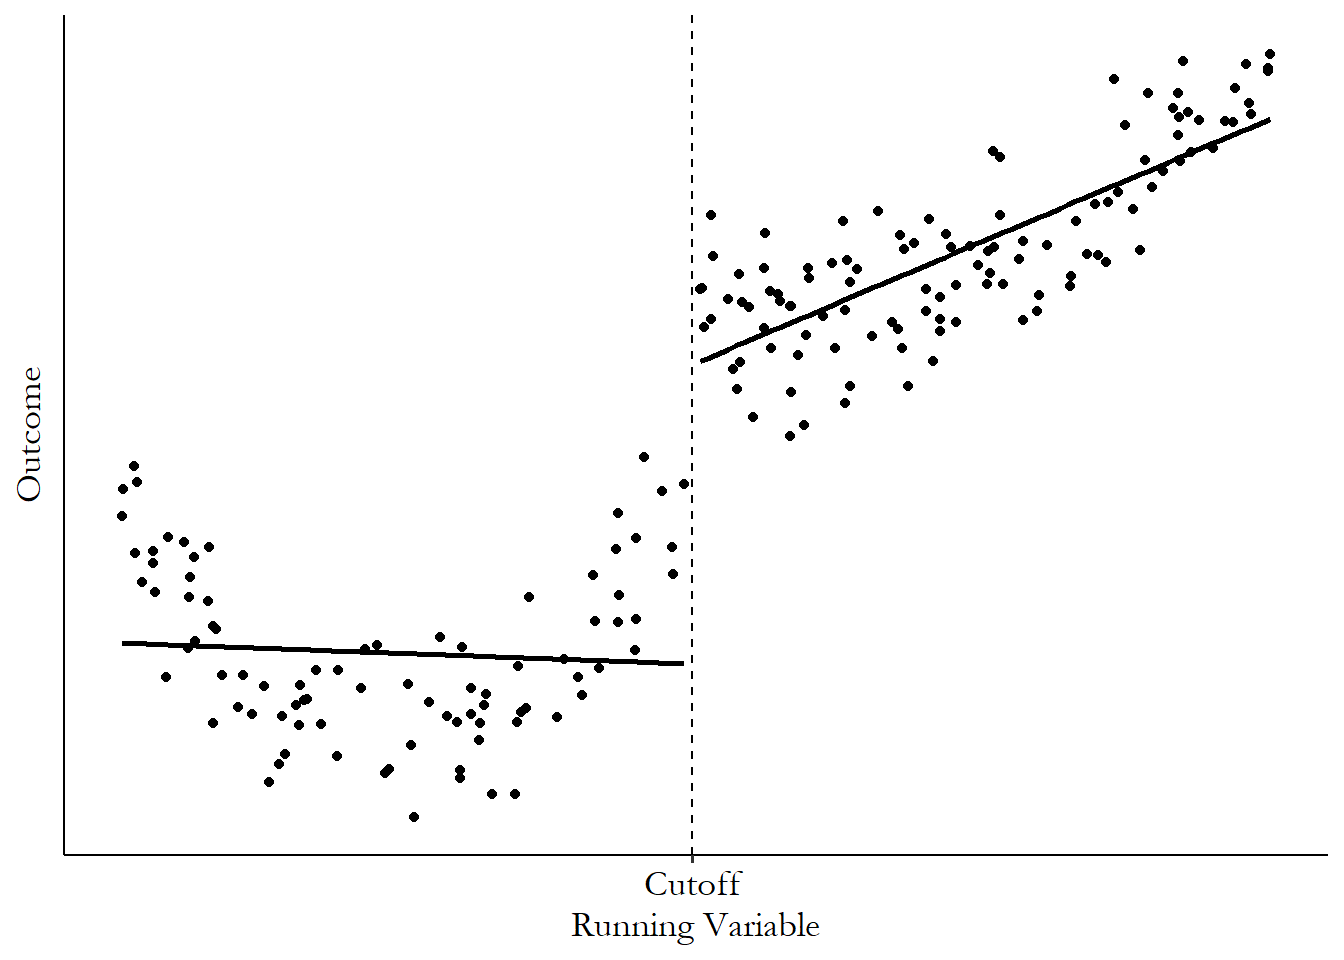
\includegraphics[width=0.85\textwidth]{figure/regressiondiscontinuity-linearrdd-1.png}
		\end{figure}
		\begin{minipage}{0.9\linewidth}
			\fontsize{8}{8pt}\selectfont
			\emph{Source:} Nick Huntington-Klein, The Effect: An Introduction to Research Design and Causality, Chapter 20
			
		\end{minipage}
	\end{center}
	
	
	
	
\end{frame}
\begin{frame}{Parametric/Global Approach}
	\begin{itemize}
		\item To \textbf{estimate the discontinuity at cutoff}, we need to model the relationship between assignment variable $A$ and outcome $Y$
		\vspace{0.2cm}
		\item Suppose that potential outcomes can be described by some reasonably smooth function $\mathrm{f}(A_i)$:
		\begin{align*}
		E[\mathrm{Y}^{0}_{i}|A_i]=\beta+ \mathrm{f}(A_i) \\
		\mathrm{Y}^{1}_{i} = \mathrm{Y}^{0}_{i}+\alpha
		\end{align*}
		
		\item We can get RD estimates by fitting:
		\begin{equation*}
		Y_i=\beta +\alpha D_i+\mathrm{f}(A_i)+\eta_i
		\end{equation*}
		
	\end{itemize}
\end{frame}
\begin{frame}{Parametric/Global Approach}
	\begin{itemize}
		
		\item Assume $\mathrm{f}(A_i)$ is a linear function of $A_{i}$
		\vspace{0.2cm}
		\item We usually do the following two settings:
		\vspace{0.2cm}
			\begin{itemize}
		\item[1] Allow the $A_i$ terms to differ on both sides of the threshold 
				\vspace{0.2cm}
			\begin{itemize}
			\item Include $A_{i}$ both individually and interacting them with $D_i$
			\vspace{0.2cm}
			\item By doing this, we can estimate $\mathrm{f}(A_i)$ on each side
						\vspace{0.2cm}
		\end{itemize}
			\item[2] Re-center $A_{i}$ at $c$: 
		\vspace{0.2cm}
		\begin{itemize}
			\item This step ensures that the treatment effect at $A_i=c$ is the coefficient on $D_i$ in a regression model 
		\end{itemize}
		
			\end{itemize}
	
	
		
		
		
		%\item The treatment effect (ATE) at $R=c$ is $\rho + \beta_1 c + \beta_2 c^{2} + ...+\beta_p c^p_i$
		%\vspace{0.2cm}
		
		
		
	\end{itemize}
\end{frame}
\begin{frame}{Parametric/Global Approach}
	\begin{itemize}
		
		
		\item Therefore, we estimate the following regression model:
	
	\begin{equation*}
		Y_i = \beta +\alpha D_i+ \gamma_1 (A_{i}-c) + \gamma_2 (A_{i}-c) \times D_i +\eta_i
	\end{equation*}
		\vspace{0.2cm}
		\begin{itemize}
			
			\item The intercept at untreated side around the cutoff: $\beta$ 
			\vspace{0.2cm}
			\item The intercept at treated side around the cutoff: $\beta +\alpha$ 
			\vspace{0.2cm}
			\item The discontinuity in outcome at cutoff: $(\beta +\alpha)$ - $\beta$ = $\alpha$
						\vspace{0.2cm}
					\begin{itemize}
			\item $\alpha=\lim_{\varepsilon\rightarrow 0}\mathrm{E}[\mathrm{Y}_{i}|A_i=c+\varepsilon] - \lim_{\varepsilon\rightarrow 0}\mathrm{E}[\mathrm{Y}_{i}|A_i=c-\varepsilon]$
				\end{itemize}
			%The treatment effect (ATE) at $R=c$ is $\rho$
			%\vspace{0.2cm}
			%\item[3] The treatment effect (ATE) at $A_i-c=s>0$ is: \\$\rho+\beta^*_1 s+\beta^*_2 s^2+...+\beta^*_p s^p$
		\end{itemize}
		
	\end{itemize}
\end{frame}
\begin{frame}{More Flexible Function}
	
	
	\begin{center}
		\begin{figure}[p]
			\centering
			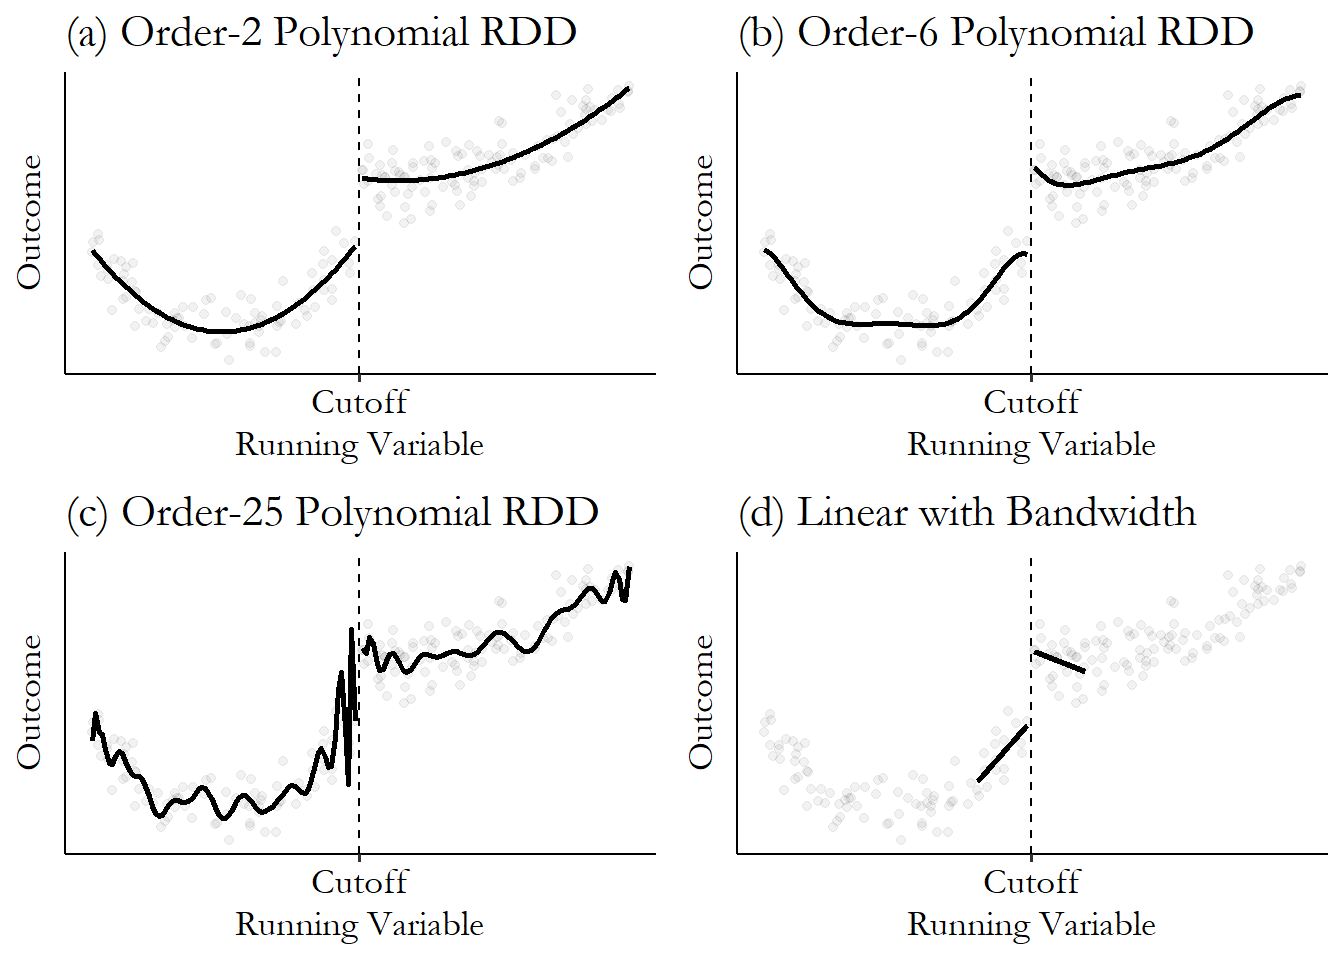
\includegraphics[width=0.85\textwidth]{figure/regressiondiscontinuity-poly-1.png}
		\end{figure}
		\begin{minipage}{0.9\linewidth}
			\fontsize{8}{8pt}\selectfont
			\emph{Source:} Nick Huntington-Klein, The Effect: An Introduction to Research Design and Causality, Chapter 20
			
		\end{minipage}
	\end{center}
	
	
	
	
\end{frame}
\begin{frame}{Parametric/Global Approach}
	\begin{itemize}
		
		
		
		\item We can use more flexible function $\mathrm{f}(A_i)$ to capture the relationship between assignment variable $A$ and outcome $Y$
									\vspace{0.2cm}
			\begin{itemize}
			\item For example, use second-order polynomial of $A$
							\vspace{0.2cm}
		\item However, more flexible function $\mathrm{f}(A_i)$ might not give better estimate of discontinuity  
					\vspace{0.2cm}
				\end{itemize}		
		\item Gelman and Imbens (2019): 
							\vspace{0.2cm}
			\begin{itemize}
		\item It's not a great idea to go above the second-order term when performing RDD
						\vspace{0.2cm}
	
	\item If there's a complex shape that needs fitting, instead try limiting the range of the data with a bandwidth and use a simpler function
		\end{itemize}
	\end{itemize}
\end{frame}

\begin{frame}{Parametric/Global Approach}{Fuzzy RDD Extension}
	\begin{itemize}
		\item In \textbf{sharp RDD}: estimate one regression directly
		\begin{equation*}
			Y_i = \beta + \alpha D_i + \gamma_1(A_i - c) + \gamma_2 D_i(A_i - c) + \eta_i
		\end{equation*}
		\vspace{0.1cm}
		\item In \textbf{fuzzy RDD}: $D_i \ne Z_i$, so we need two regressions
		\vspace{0.2cm}
		\begin{itemize}
			\item \textbf{First Stage} (effect of crossing cutoff on treatment):
			\begin{equation*}
				D_i = \alpha_1 + \rho_1 Z_i + \gamma_1(A_i-c) + \delta_1 Z_i(A_i-c) + \upsilon_i
			\end{equation*}
			\vspace{0.1cm}
			\item \textbf{Reduced Form} (intent-to-treat, effect on outcome):
			\begin{equation*}
				Y_i = \alpha_2 + \rho_2 Z_i + \gamma_2(A_i-c) + \delta_2 Z_i(A_i-c) + \eta_i
			\end{equation*}
			% \vspace{0.1cm}
			% \item \textbf{LATE} via 2SLS: instrument $D_i$ with $Z_i$
			% \begin{equation*}
			% 	\widehat{\mathrm{LATE}} = \frac{\hat{\rho}_2}{\hat{\rho}_1} = \mathrm{E}[\mathrm{Y}^1_i - \mathrm{Y}^0_i \mid \mathrm{D}^1_i > \mathrm{D}^0_i,\, A_i = c]
			% \end{equation*}
		\end{itemize}
	\end{itemize}
\end{frame}


\begin{frame}{Fuzzy RDD Estimation}{2SLS --- How It Works}
	\begin{itemize}
		\item \textbf{Two-Stage Least Squares (2SLS)} removes the part of $D_i$ correlated with unobservables
		\vspace{0.15cm}
		\item \textbf{Stage 1} --- regress treatment on the instrument and controls:
		\begin{equation*}
			D_i = \alpha_1 + \rho_1 Z_i + \gamma_1(A_i-c) + \delta_1 Z_i(A_i-c) + \upsilon_i
		\end{equation*}
		Obtain fitted values $\hat{D}_i = \hat{\alpha}_1 + \hat{\rho}_1 Z_i + \hat{\gamma}_1(A_i-c) + \hat{\delta}_1 Z_i(A_i-c)$
		\vspace{0.15cm}
		\item \textbf{Stage 2} --- regress outcome on \emph{predicted} treatment:
		\begin{equation*}
			Y_i = \alpha_2 + \rho_2 \hat{D}_i + \gamma_2(A_i-c) + \delta_2 Z_i(A_i-c) + \eta_i
		\end{equation*}
		$\hat{\rho}_2$ is the \textbf{LATE} estimate
	\end{itemize}
\end{frame}


\begin{frame}{Fuzzy RDD Estimation}{2SLS --- Intuition and LATE}
	\begin{itemize}
		\item \textbf{Intuition}: $\hat{D}_i$ retains \emph{only} the variation in treatment driven by the cutoff $Z_i$ (exogenous) and discards the part driven by unobservables (e.g.\ ability)
		\vspace{0.2cm}
		\begin{itemize}
			\item OLS uses all variation in $D_i$, including the confounded part $\Rightarrow$ biased
			\vspace{0.1cm}
			\item 2SLS uses only the ``as-good-as-random'' cutoff-driven variation $\Rightarrow$ LATE
		\end{itemize}
		\vspace{0.3cm}
		\item \textbf{What does 2SLS identify?}
		\begin{block}{Local Average Treatment Effect (LATE)}
			\begin{equation*}
				\hat{\rho}_2 \;\xrightarrow{p}\; \mathrm{E}\!\left[\mathrm{Y}^1_i - \mathrm{Y}^0_i \;\middle|\; \mathrm{D}^1_i > \mathrm{D}^0_i,\; A_i = c\right]
			\end{equation*}
		\end{block}
		The causal effect of treatment for \textbf{compliers} at the cutoff $c$
		% \vspace{0.2cm}
		% \item \textbf{Note}: use \texttt{ivregress 2sls} (Stata) or \texttt{ivreg()} (R) --- running two separate OLS steps manually gives \emph{wrong} standard errors
	\end{itemize}
\end{frame}



% \begin{frame}{Fuzzy RDD Estimation}{2SLS --- How It Works}
% 	\begin{itemize}
% 		\item \textbf{Two-Stage Least Squares (2SLS)} removes the part of $D_i$ correlated with unobservables
% 		\vspace{0.15cm}
% 		\item \textbf{Stage 1} --- regress treatment on the instrument and controls:
% 		\begin{equation*}
% 			D_i = \alpha_1 + \rho_1 Z_i + \gamma_1(A_i-c) + \delta_1 Z_i(A_i-c) + \upsilon_i
% 		\end{equation*}
% 		Obtain fitted values $\hat{D}_i = \hat{\alpha}_1 + \hat{\rho}_1 Z_i + \hat{\gamma}_1(A_i-c) + \hat{\delta}_1 Z_i(A_i-c)$
% 		\vspace{0.15cm}
% 		\item \textbf{Stage 2} --- regress outcome on \emph{predicted} treatment:
% 		\begin{equation*}
% 			Y_i = \alpha_2 + \rho_2 \hat{D}_i + \gamma_2(A_i-c) + \delta_2 Z_i(A_i-c) + \eta_i
% 		\end{equation*}
% 		$\hat{\rho}_2$ is the \textbf{LATE} estimate
% 		\vspace{0.15cm}
% 		\item \textbf{Intuition}: $\hat{D}_i$ retains only the variation in treatment driven by the cutoff $Z_i$ (exogenous) and discards the part driven by unobservables (e.g.\ ability)
% 		\vspace{0.1cm}
% 		\begin{itemize}
% 			\item OLS uses all variation in $D_i$, including the confounded part $\Rightarrow$ biased
% 			\item 2SLS uses only the ``as-good-as-random'' cutoff-driven variation $\Rightarrow$ LATE
% 		\end{itemize}
% 		\vspace{0.1cm}
% 		\item \textbf{Note}: in practice use \texttt{ivregress 2sls} / \texttt{ivreg()} --- running two separate OLS steps gives wrong standard errors
% 	\end{itemize}
% \end{frame}


\begin{frame}{Sharp RDD Estimation}{Nonparametric/Local Approach}
	\begin{itemize}

		\item The core idea of RDD is to compare outcomes just above and just below the cutoff $c$.
		\vspace{0.2cm}
		\item Nonparametric/local method:
		\vspace{0.2cm}
		\begin{itemize}
			\item We do \textbf{not} assume a specific global functional form for the relationship between the outcome $Y$ and the assignment variable $A$ over their entire range. 
						\vspace{0.2cm}
					\begin{itemize}
			\item This is what "nonparametric" means in this context.
			\vspace{0.2cm}
					\end{itemize}
			\item Instead, we focus the analysis \textbf{locally}, using only observations close to the cutoff $c$.
			\vspace{0.2cm}
			\item We compare treated and untreated observations that fall within a specific \textbf{bandwidth ($h$)} around the cutoff.
		\end{itemize}
		
	\end{itemize}
		
		

\end{frame}
\begin{frame}{Sharp RDD Estimation}{Nonparametric/Local Approach}
\begin{itemize}
	%\item As mentioned, the "nonparametric" aspect means we avoid assuming a global functional form for $E[Y_i | A_i = a]$.
	%\vspace{0.2cm}
	%\item However, we still need a way to estimate the potential jump in $Y$ precisely *at* the cutoff $c$.
	%\vspace{0.2cm}
	\item Key insight: within a \textbf{sufficiently small local window (bandwidth $h$)} around the cutoff $c$, even if the true relationship is complex globally.
	\begin{itemize}
		\vspace{0.2cm}
	\item It can often be well \textbf{approximated by a simple linear function}.
	\vspace{0.2cm}
\end{itemize}
	\item Therefore, we use \textbf{Local linear regression}:
			\vspace{0.2cm}
	\begin{itemize}
		\item This involves fitting separate linear regressions on each side of the cutoff, but \textit{only} using data within the bandwidth $h$.
		\vspace{0.2cm}
		%\item This allows for different intercepts and slopes on either side of $c$.
		%\vspace{0.2cm}
		\item Optionally, kernel functions can be used to give more weight to observations closer to the cutoff.
	\end{itemize}
%	\item This approach is generally preferred over simply comparing means in bins next to the cutoff, as it helps reduce potential bias near the boundary of the bandwidth.
\end{itemize}
\end{frame}
\begin{frame}{Sharp RDD Estimation}{Implementing Local Linear Regression}
	\begin{itemize}
		\item Specifically, we estimate the following regression model \textbf{using only observations within the chosen bandwidth $h$}:
		\begin{equation*}
			Y_i = \beta +\alpha D_i+ \gamma_1 (A_{i}-c) + \gamma_2 (A_{i}-c) \times D_i +\eta_i
		\end{equation*}
		\item This linear model is just a \textbf{local approximation} of the relationship near the cutoff $c$, within the bandwidth $h$. 
				\vspace{0.2cm}
			\begin{itemize}
		\item It is \textit{not} a global assumption about the functional form.
		\vspace{0.2cm}
			\end{itemize}
%		\item Interpretation of coefficients:
%		\begin{itemize}
%			\item $D_i$: Treatment indicator (=1 if $A_i \ge c$, 0 if $A_i < c$).
%			\item $A_i - c$: Assignment variable centered at the cutoff.
%			\item $\beta$: The estimated intercept for the control group ($D_i=0$) at the cutoff ($A_i = c$).
%			\item $\alpha$: \textbf{The RDD Treatment Effect}. This estimates the jump (discontinuity) in the outcome $Y$ at the cutoff $c$ comparing the treated ($D_i=1$) to the control ($D_i=0$) group. \textbf{This is the parameter of primary interest.}
%			\item $\gamma_1$: The estimated slope of the relationship between $Y$ and $(A_i-c)$ for the control group ($D_i=0$) within the bandwidth.
%			\item $\gamma_2$: The estimated \textit{change} in slope for the treated group ($D_i=1$) compared to the control group, within the bandwidth. (The slope for the treated group is $\gamma_1 + \gamma_2$).
%		\end{itemize}
		\item The estimated coefficient $\hat{\alpha}$ provides the RDD estimate of the treatment effect.
	\end{itemize}
\end{frame}
\begin{frame}{Bandwidth}
	
	
	\begin{center}
		\begin{figure}[p]
			\centering
			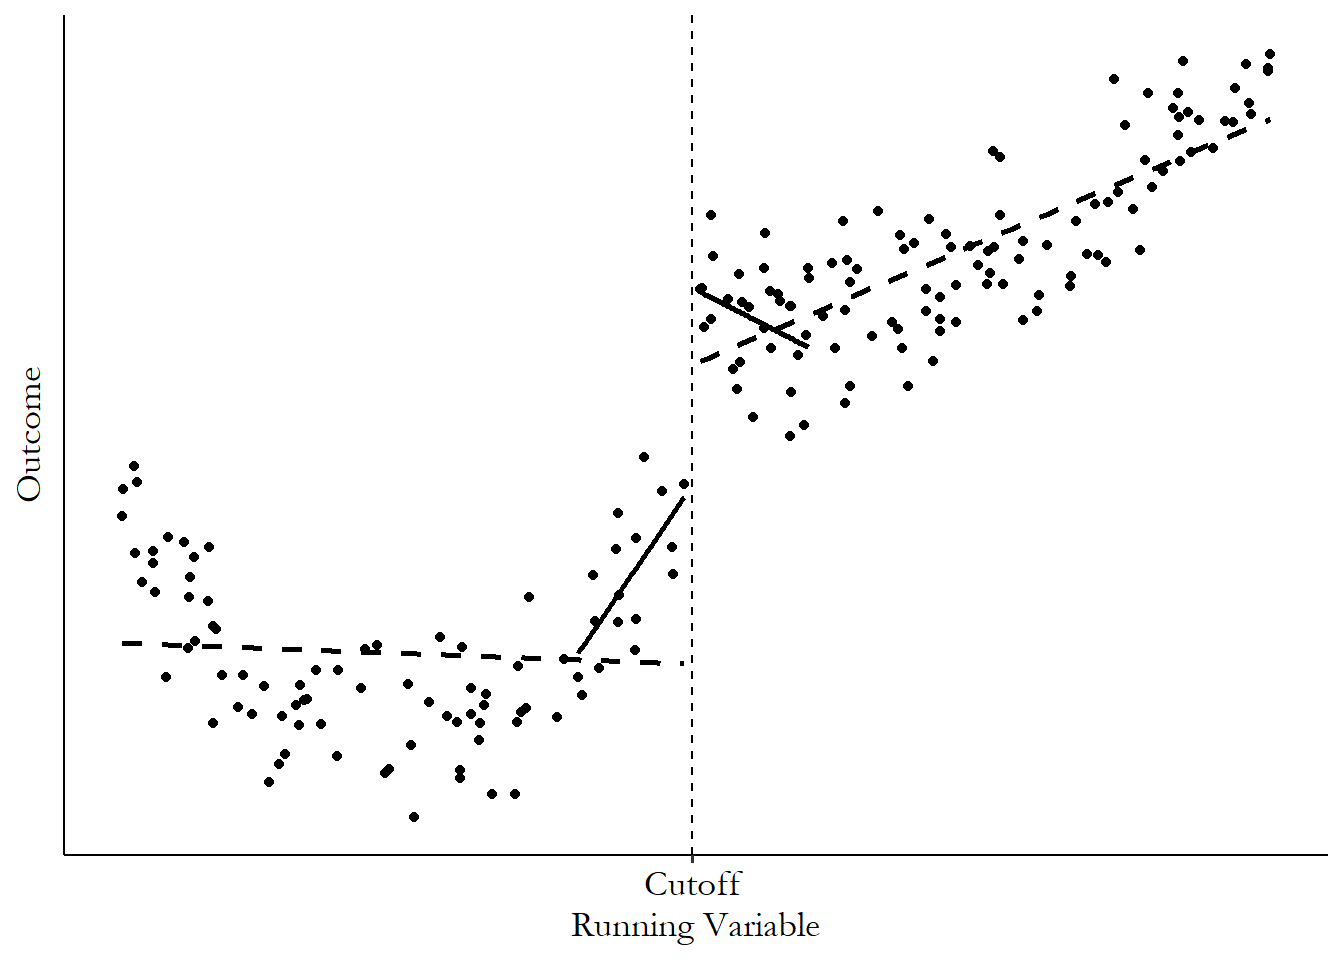
\includegraphics[width=0.85\textwidth]{figure/regressiondiscontinuity-localproblems-1.png}
		\end{figure}
		\begin{minipage}{0.9\linewidth}
			\fontsize{8}{8pt}\selectfont
			\emph{Source:} Nick Huntington-Klein, The Effect: An Introduction to Research Design and Causality, Chapter 20
			
		\end{minipage}
	\end{center}
	
	
	
	
\end{frame}
\begin{frame}{Sharp RDD Estimation}{Nonparametric/Local Approach}
	\begin{itemize}
		\item The main challenge of nonparametric approach is to \textbf{choose a bandwidth} 
		\vspace{0.2cm}
		\item There is essentially a trade-off between \textbf{bias} and \textbf{precision} (efficiency) 
		\vspace{0.2cm}
		\item Use a larger bandwidth:  
		\vspace{0.2cm}
		\begin{itemize}
			\item Since more data points are used in the regression
			\vspace{0.2cm}	
			\item Get more \textbf{precise} treatment effect estimates
			\vspace{0.2cm}
			\item But use data points far from cutoff 
			\vspace{0.2cm}
			%\item Linear specification is less likely to be accurate
			%\vspace{0.2cm}
			\item The estimated treatment effect could be \textbf{biased}
		\end{itemize}
		
		
	\end{itemize}
\end{frame}
\begin{frame}{Sharp RDD Estimation}{How to Choose Bandwidth}
	\begin{itemize}
		\item[1.] \textbf{Cross-Validation (CV) Procedure}:
		\vspace{0.2cm}
		\begin{itemize}
			\item Aims to select $h$ that minimizes prediction errors of the RDD model specifically in the neighborhood of the cutoff $c$.
			%\vspace{0.2cm}
			%\item This often involves minimizing a cross-validated criterion, such as the sum of squared residuals, derived from local polynomial RDD model fits.
		\end{itemize}
		\vspace{0.3cm} % Adjusted spacing for clarity
		\item[2.] \textbf{Plug-In Procedure}:
		\vspace{0.2cm}
		\begin{itemize}
			\item Derives a formula for the optimal bandwidth ($h_{opt}$) by analytically minimizing an (Asymptotic) Mean Squared Error for the RDD treatment effect estimator (e.g., $\hat{\alpha}$)
			
			%expression for the RDD treatment effect estimator (e.g., $\hat{\alpha}$).
			\vspace{0.2cm}
			\begin{itemize}
				%\item This AMSE typically reflects a trade-off between the squared bias and the variance of the estimator.
				%\vspace{0.2cm}
				\item The $h_{opt}$ formula depends on some unknown data characteristics at the cutoff $c$ (like local trends and data variability). 
				\vspace{0.2cm}
				\item These must first be estimated from your data, often using a "pilot" bandwidth.
				\vspace{0.2cm}
			\end{itemize}		
			\item See, e.g., Imbens and Kalyanaraman (2012), Calonico, Cattaneo, and Titiunik (2014).
		\end{itemize}
	\end{itemize}
\end{frame}
\begin{frame}{Sharp RDD Estimation}{Nonparametric/Local Approach}
	\begin{itemize}
		\item In practice, we also use a specific kernel function to weight observations more heavily around cutoff
		
					\vspace{0.2cm}
		\item A very commonly-used kernel in regression discontinuity is the \textbf{triangular kernel}
		
\begin{equation}
	K(A) = 
	\begin{cases} 
		1 - \frac{\left| A_{i} - c \right|}{h} & \text{for}\: c - h < A_{i} < c + h, \\
		0 & \text{otherwise.}
	\end{cases}
\end{equation}

%Therefore, we estimate the following local linear regression
		
	\end{itemize}
\end{frame}
\begin{frame}{Triangular Kernel Function}
	
	
	\begin{center}
		\begin{figure}[p]
			\centering
			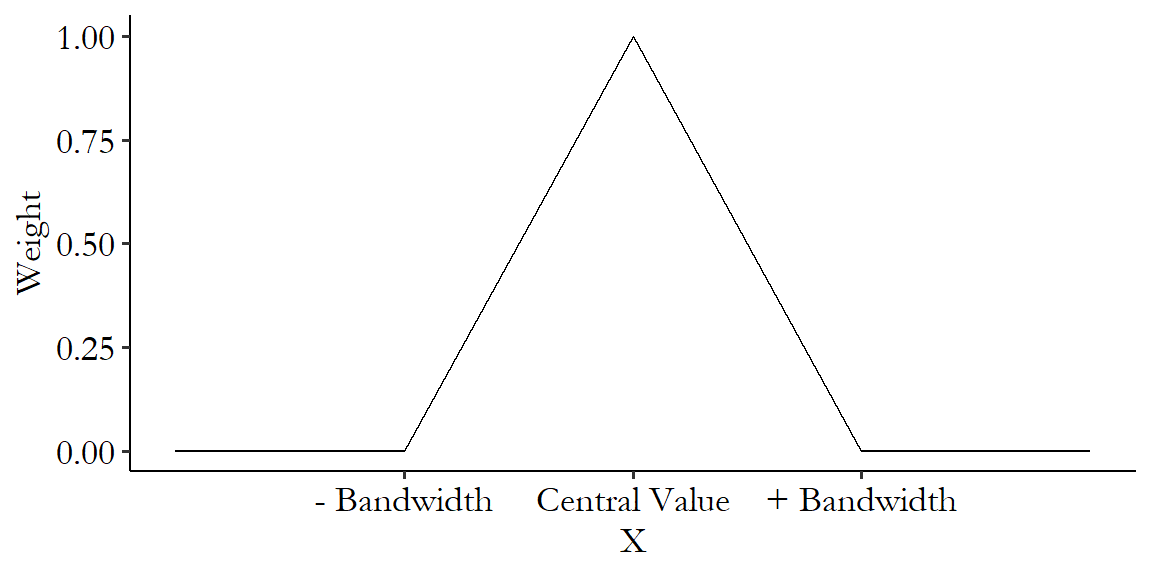
\includegraphics[width=0.9\textwidth]{figure/regressiondiscontinuity-kernel-1.png}
		\end{figure}
		\begin{minipage}{0.9\linewidth}
			\fontsize{8}{8pt}\selectfont
			\emph{Source:} Nick Huntington-Klein, The Effect: An Introduction to Research Design and Causality, Chapter 20
			
		\end{minipage}
	\end{center}
	
	
	
	
\end{frame}




\begin{frame}{Nonparametric/Local Approach}{Fuzzy RDD Extension}
	\begin{itemize}
		\item In \textbf{sharp RDD}: estimate one local regression within bandwidth $h$
		\begin{equation*}
			Y_i = \beta + \alpha D_i + \gamma_1(A_i - c) + \gamma_2 D_i(A_i-c) + \eta_i, \quad |A_i-c|\leq h
		\end{equation*}
		\vspace{0.1cm}
		\item In \textbf{fuzzy RDD}: $D_i \ne Z_i$, so we need two local regressions within $|A_i - c|\leq h$
		\vspace{0.2cm}
		\begin{itemize}
			\item \textbf{First Stage}:
			\begin{equation*}
				D_i = \alpha_1 + \rho_1 Z_i + \gamma_1(A_i-c) + \delta_1 Z_i(A_i-c) + \upsilon_i
			\end{equation*}
			\vspace{0.1cm}
			\item \textbf{Reduced Form}:
			\begin{equation*}
				Y_i = \alpha_2 + \rho_2 Z_i + \gamma_2(A_i-c) + \delta_2 Z_i(A_i-c) + \eta_i
			\end{equation*}
		\end{itemize}
		\vspace{0.1cm}
		\item Both regressions weighted by triangular kernel $K_h(A_i - c) = \bigl(1 - |A_i-c|/h\bigr)/h$
	\end{itemize}
\end{frame}

\begin{frame}{Fuzzy RDD Estimation}{Local 2SLS --- How It Works}
	\begin{itemize}
		\item Same 2SLS logic as parametric, but estimated \emph{locally} within bandwidth $h$
		\vspace{0.15cm}
		\item \textbf{Stage 1} --- regress treatment on instrument and controls (within $|A_i-c|\leq h$):
		\begin{equation*}
			D_i = \alpha_1 + \rho_1 Z_i + \gamma_1(A_i-c) + \delta_1 Z_i(A_i-c) + \upsilon_i
		\end{equation*}
		Obtain fitted values $\hat{D}_i$
		\vspace{0.15cm}
		\item \textbf{Stage 2} --- regress outcome on \emph{predicted} treatment (within $|A_i-c|\leq h$):
		\begin{equation*}
			Y_i = \alpha_2 + \rho_2 \hat{D}_i + \gamma_2(A_i-c) + \delta_2 Z_i(A_i-c) + \eta_i
		\end{equation*}
		$\hat{\rho}_2$ is the \textbf{LATE} estimate
		\vspace{0.15cm}
		\item \textbf{Bandwidth} $h$: MSE-optimal selection balances bias and variance
		\vspace{0.1cm}
		\item \textbf{Inference}: use bias-corrected robust CI \citep{Calonico2014}
	\end{itemize}
\end{frame}



\title[]
{Empirical Example: Stata/R}

\author
{}

\institute{}

\date
{}

\begin{frame}{}
	\titlepage
\end{frame}

\begin{frame}{Bleemer \& Mehta (2022)}{Motivation}
	
	Zachary Bleemer and Aashish Mehta (2022) ``\textbf{Will Studying Economics Make You Rich? A Regression Discontinuity Analysis of the Returns to College Major}", American Economic Journal: Applied Economics
	
	\begin{itemize}
				\vspace{0.2cm}
		\item Examine the causal effect of majoring in economics on early-career earnings
		
		\vspace{0.2cm}
		\item Key Research Questions:
				\vspace{0.2cm}
		\begin{itemize}
			\item What is the wage return to studying economics?
					\vspace{0.2cm}
			\item How does access to economics major affect students' career paths?
					\vspace{0.2cm}
			\item Do observational wage differences reflect causal effects?
		\end{itemize}
	\end{itemize}
	
\end{frame}
\begin{frame}{Empirical Example: Bleemer \& Mehta (2022)}{Motivation}
	\begin{itemize}
		\item College graduates with economics degrees earn substantially higher wages
		\vspace{0.2cm}
		\begin{itemize}
			\item Median wage of \$90,000 for economics majors vs. \$65,000 for other social sciences
		\end{itemize}
		
		\vspace{0.2cm}
		\item However, estimating causal effects is challenging due to:
					\vspace{0.2cm}
		\begin{itemize}
			\item Students' nonrandom selection into majors
			\vspace{0.2cm}
			\item Universities' admissions and grade requirements
		\end{itemize}
		
		\vspace{0.2cm}
		\item Study exploits a GPA threshold policy at UC Santa Cruz that restricted access to the economics major
		\begin{itemize}
						\vspace{0.2cm}
			\item Students needed 2.8 GPA in Economics 1 \& 2 to declare major
		\end{itemize}
		
	\end{itemize}
\end{frame}
\begin{frame}{Empirical Example: Bleemer \& Mehta (2022)}{Identification Strategy}
	\begin{itemize}
		\item \textbf{Fuzzy RDD}: Exploits GPA threshold (2.8) in Economics 1 and 2 for major access
		
		\vspace{0.2cm}
		\begin{equation*}
			\begin{aligned}
				\alpha_{FRD} &=\dfrac{\lim_{\varepsilon\rightarrow 0}\mathrm{E}[Y_{i}|A_{i}=c+\varepsilon]-\lim_{\varepsilon\rightarrow 0}\mathrm{E}[Y_{i}|A_{i}=c-\varepsilon]}{\lim_{\varepsilon\rightarrow 0}\mathrm{E}[D_{i}|A_{i}=c+\varepsilon]-\lim_{\varepsilon\rightarrow 0}\mathrm{E}[D_{i}|A_{i}=c-\varepsilon]} 
			\end{aligned}
		\end{equation*} 
		
		\item Where:
		\begin{itemize}
					\vspace{0.2cm}
			\item $Y_i$: Early-career wages (2017-2018)
					\vspace{0.2cm}
			\item $A_i$: Average GPA in Economics 1 \& 2
					\vspace{0.2cm}
			\item $D_i$: Economics major indicator
					\vspace{0.2cm}
			\item $c$: GPA threshold (2.8)
		\end{itemize}
	\end{itemize}
\end{frame}
\begin{frame}{Empirical Example: Bleemer \& Mehta (2022)}{Empirical Specification}
	\begin{itemize}
		\item \textbf{First Stage}:
		\begin{equation*}
			D_i = \alpha_1 + \rho_1 Z_i + \mathrm{f}_1(A_i) + \upsilon_i
		\end{equation*}
		
		\item \textbf{Reduced Form}:
		\begin{equation*}
			Y_i = \alpha_2 + \rho_2 Z_i + \mathrm{f}_2(A_i) + \eta_i
		\end{equation*}
		
		\item Where:
		\begin{itemize}
			\item $D_i$: Economics major indicator
			\item $Z_i = 1(A_i \geq 2.8)$: Treatment eligibility
			\item $A_i$: Average GPA in Economics 1 \& 2
			\item $\mathrm{f}_1(.), \mathrm{f}_2(.)$: Linear functions of GPA
		\end{itemize}
		
		\vspace{0.2cm}
		\item \textbf{Fuzzy RD Estimate}:
		\begin{equation*}
			\alpha_{FRD} = \frac{\rho_2}{\rho_1} = \mathrm{E}[ \mathrm{Y}^1_i - \mathrm{Y}^0_i | \mathrm{D}^1_i > \mathrm{D}^0_i, A_i=2.8]
		\end{equation*}
	\end{itemize}
\end{frame}

\begin{frame}{Data and Program}{STATA Implementation}
	\begin{itemize}
		\item See \texttt{RDD\_fuzzy.do}
		\vspace{0.2cm}
		\item Use \texttt{RDD.dta} (calibrated to the paper)
		\vspace{0.2cm}
		\item Install required packages:
		\begin{itemize}
			\vspace{0.2cm}
			\item \texttt{binscatter.ado}
			\item \texttt{rdrobust.ado}
			\item \texttt{rddensity.ado}
			\item \texttt{DCdensity.ado}
		\end{itemize}
		\vspace{0.2cm}
		\item Key steps:
		\begin{enumerate}
			\vspace{0.2cm}
			\item Graphical analysis (first stage, reduced form, covariate balance)
			\item Sorting/manipulation test
			\item Preparation for estimation (centered running variable)
			\item Parametric estimation (first stage, reduced form, 2SLS)
			\item Nonparametric estimation (\texttt{rdrobust fuzzy()})
			\item Robustness checks
		\end{enumerate}
	\end{itemize}
\end{frame}


\begin{frame}{Data and Program}{R Implementation}
	\begin{itemize}
		\item See \texttt{RDD\_fuzzy.R}
		\vspace{0.2cm}
		\item Use \texttt{RDD.dta} (calibrated to the paper)
		\vspace{0.2cm}
		\item Install required packages:
		\begin{itemize}
			\vspace{0.2cm}
			\item \texttt{haven}, \texttt{dplyr} (data handling)
			\item \texttt{rdrobust} (\texttt{rdrobust}, \texttt{rdplot})
			\item \texttt{rddensity} (manipulation test)
			\item \texttt{AER} (\texttt{ivreg} for 2SLS)
		\end{itemize}
		\vspace{0.2cm}
		\item Key steps: same as STATA
		\begin{enumerate}
			\vspace{0.2cm}
			\item Graphical analysis (\texttt{rdplot})
			\item Sorting test (\texttt{rddensity})
			\item Preparation for estimation (\texttt{mutate})
			\item Parametric estimation (\texttt{lm} + \texttt{ivreg})
			\item Nonparametric estimation (\texttt{rdrobust} with \texttt{fuzzy=})
			\item Robustness checks
		\end{enumerate}
	\end{itemize}
\end{frame}


\begin{frame}{Step 1: Graphical Analysis}{First Stage}
	\begin{itemize}
		\item In fuzzy RDD, \textbf{always} produce two RD plots before any regression
		\vspace{0.2cm}
		\item \textbf{First stage}: plot the \textbf{treatment} ($D_i$ = economics major)
		against the \textbf{running variable} ($A_i$ = GPA in Econ 1 \& 2)
		\vspace{0.2cm}
		\begin{itemize}
			\item Construct bins, average the treatment within bins on each side of the cutoff
			\vspace{0.2cm}
			\item Inspect whether D (economics major) \textbf{jumps} at GPA = 2.8
			\vspace{0.2cm}
			\item The size of the jump is the \textbf{first-stage estimate} ($\hat{\rho}_1$)
			\vspace{0.2cm}
			\item Bleemer \& Mehta (2022): students just above 2.8 GPA were
			\textbf{36 percentage points} more likely to major in economics
		\end{itemize}
	\end{itemize}
\end{frame}


\begin{frame}[fragile]{STATA: Step 1}{First Stage}
	\begin{itemize}
		\item Example (first stage graph):
\begin{lstlisting}
use "RDD.dta", clear
binscatter econ_major gpa_econ, n(50) rd(2.8) linetype(lfit) /*
*/ xtitle("GPA in Introductory Economics")                   /*
*/ ytitle("P(Economics Major)")                              /*
*/ title("First Stage: GPA Cutoff and Economics Enrollment")
graph export figure/econ_fs.png, replace
\end{lstlisting}
		\vspace{0.2cm}
		\item \textbf{econ\_major}: treatment $D_i$ on the y-axis
		\vspace{0.2cm}
		\item \textbf{gpa\_econ}: running variable $A_i$ on the x-axis
		\vspace{0.2cm}
		\item \textbf{rd(2.8)}: split sample at the GPA cutoff
		\vspace{0.2cm}
		\item \textbf{linetype(lfit)}: fit a linear regression line on each side
	\end{itemize}
\end{frame}


\begin{frame}[fragile]{R: Step 1}{First Stage}
\begin{lstlisting}[style=r-style]
library(haven); library(rdrobust); library(dplyr)
data   <- read_dta("RDD.dta")
cutoff <- 2.8
# First stage: P(Economics Major) by GPA
rdplot(y = data$econ_major, x = data$gpa_econ, c = cutoff,
       title   = "First Stage: GPA Cutoff and Economics Enrollment",
       x.label = "GPA in Introductory Economics",
       y.label = "P(Economics Major)")
\end{lstlisting}
\end{frame}

\begin{frame}{Empirical Example: Bleemer \& Mehta (2022)}{First Stage}
	
	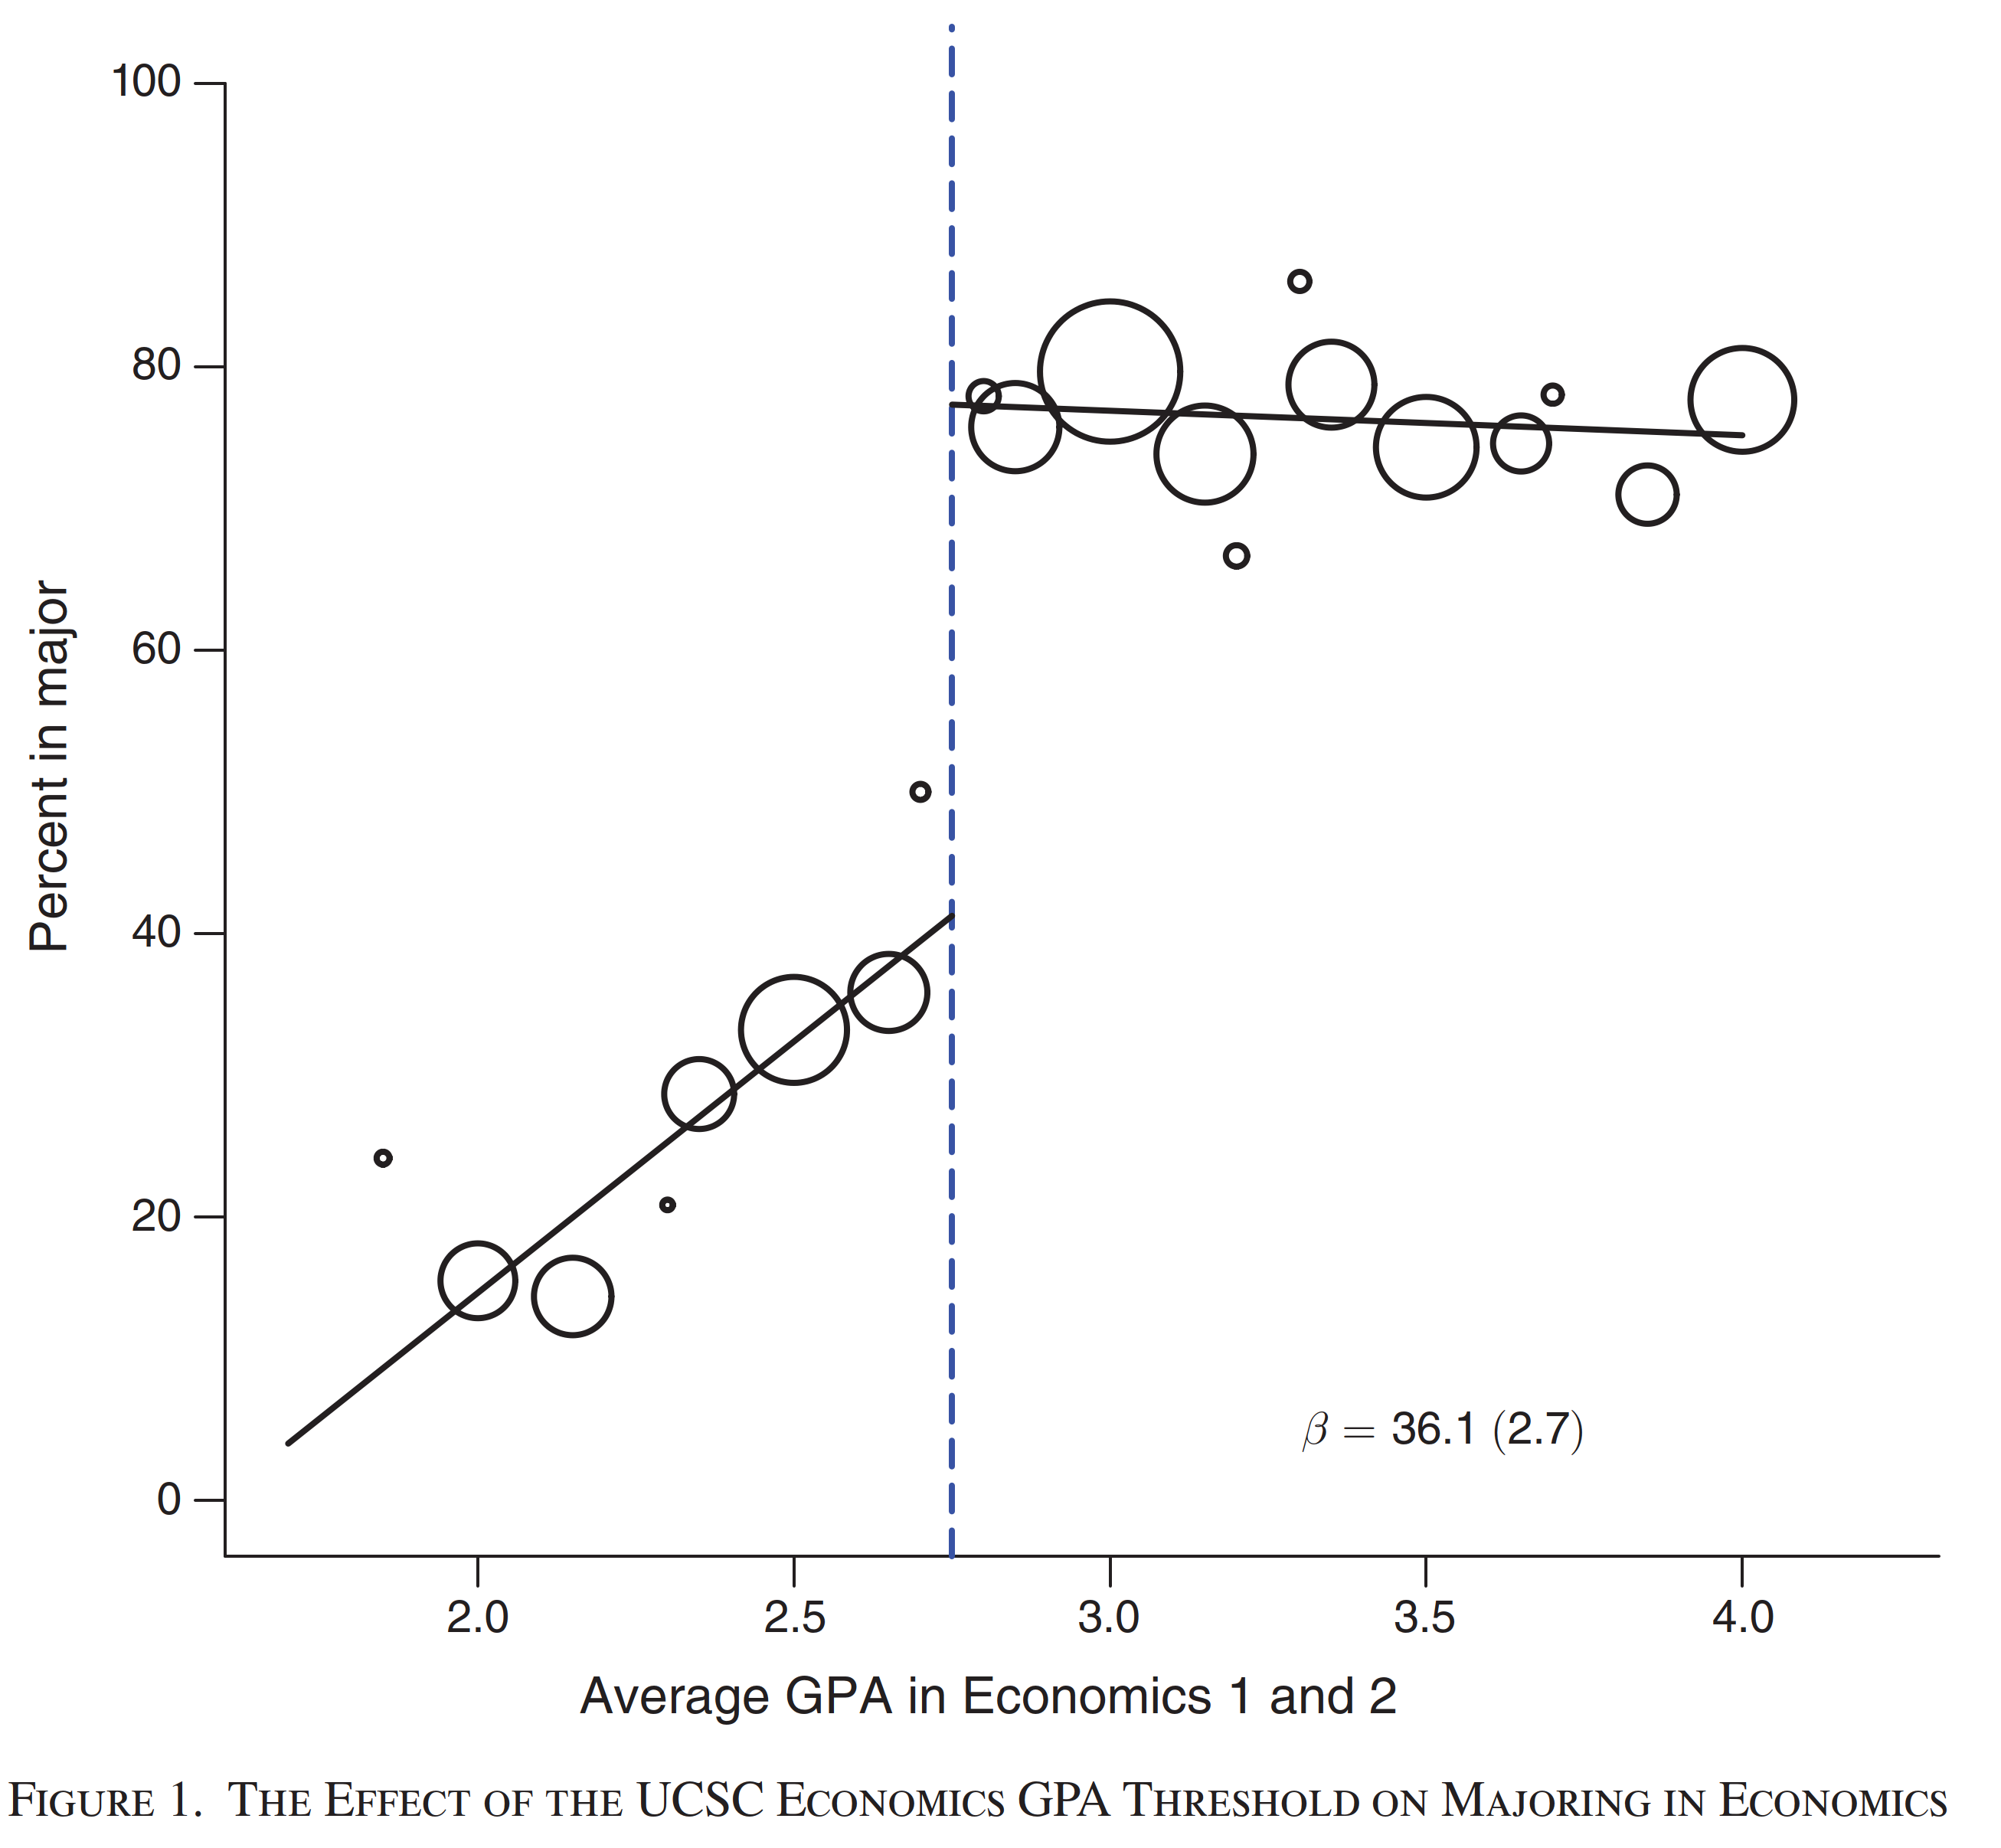
\includegraphics[width=0.60\textwidth]{figure/RD_econ_major_f1.png}
	
	
\end{frame}
\begin{frame}{Empirical Example: Bleemer \& Mehta (2022)}{First Stage}
	\begin{itemize}
		\item Students just above 2.8 GPA threshold were:
		\vspace{0.2cm}
		\begin{itemize}
			\item 36 percentage points more likely to major in economics
			\vspace{0.2cm}
			\item Most would have otherwise majored in other social sciences
			\vspace{0.2cm}
		\end{itemize}
		
		%		\item Compliers are representative of economics majors:
		%				\vspace{0.2cm}
		%		\begin{itemize}
			%			\item 36\% female (vs. 41\% all econ majors)
			%					\vspace{0.2cm}
			%			\item 41\% Asian (vs. 44\% all econ majors)
			%					\vspace{0.2cm}
			%			\item SAT scores at 41st percentile of econ majors
			%		\end{itemize}
	\end{itemize}
\end{frame}

\begin{frame}{Step 1: Graphical Analysis}{Reduced Form}
	\begin{itemize}
		\item \textbf{Reduced form}: plot the \textbf{outcome} ($Y_i$ = log wages)
		against the \textbf{running variable} ($A_i$ = GPA)
		\vspace{0.2cm}
		\begin{itemize}
			\item Shows the \textbf{intent-to-treat (ITT)} effect:
			the total effect of \emph{eligibility} ($Z_i$) on wages
			\vspace{0.2cm}
			\item The jump at GPA = 2.8 is the \textbf{reduced-form estimate} ($\hat{\rho}_2$)
			\vspace{0.2cm}
			\item LATE $= \hat{\rho}_2 / \hat{\rho}_1$ (Wald estimator)
			\vspace{0.2cm}
			\item Bleemer \& Mehta (2022): wages rise $\approx$ 14\% at the cutoff (ITT)
		\end{itemize}
	\end{itemize}
\end{frame}


\begin{frame}[fragile]{STATA: Step 1}{Reduced Form}
	\begin{itemize}
		\item Example (reduced form graph):
\begin{lstlisting}
binscatter logwage_1718 gpa_econ if employed_1718, /*
*/ n(50) rd(2.8) linetype(lfit)                    /*
*/ xtitle("GPA in Introductory Economics")         /*
*/ ytitle("Log Wages 2017-2018")                   /*
*/ title("Reduced Form: GPA Cutoff and Wages")
graph export figure/econ_rf.png, replace
\end{lstlisting}
		\vspace{0.2cm}
		\item \textbf{if employed\_1718}: restrict to employed workers
		(wages only observed for employed)
		\vspace{0.2cm}
		\item A visible jump at GPA = 2.8 indicates that the GPA cutoff
		affects wages through the economics major pathway
	\end{itemize}
\end{frame}


\begin{frame}[fragile]{R: Step 1}{Reduced Form}
\begin{lstlisting}[style=r-style]
data_emp <- data |> filter(employed_1718 == 1, !is.na(logwage_1718))
# Reduced form: Log wages by GPA
rdplot(y = data_emp$logwage_1718, x = data_emp$gpa_econ, c = cutoff,
       title   = "Reduced Form: GPA Cutoff and Log Wages",
       x.label = "GPA in Introductory Economics",
       y.label = "Log Wages (2017-2018)")
\end{lstlisting}
\end{frame}

\begin{frame}{Empirical Example: Bleemer \& Mehta (2022)}{Second Stage}
	
	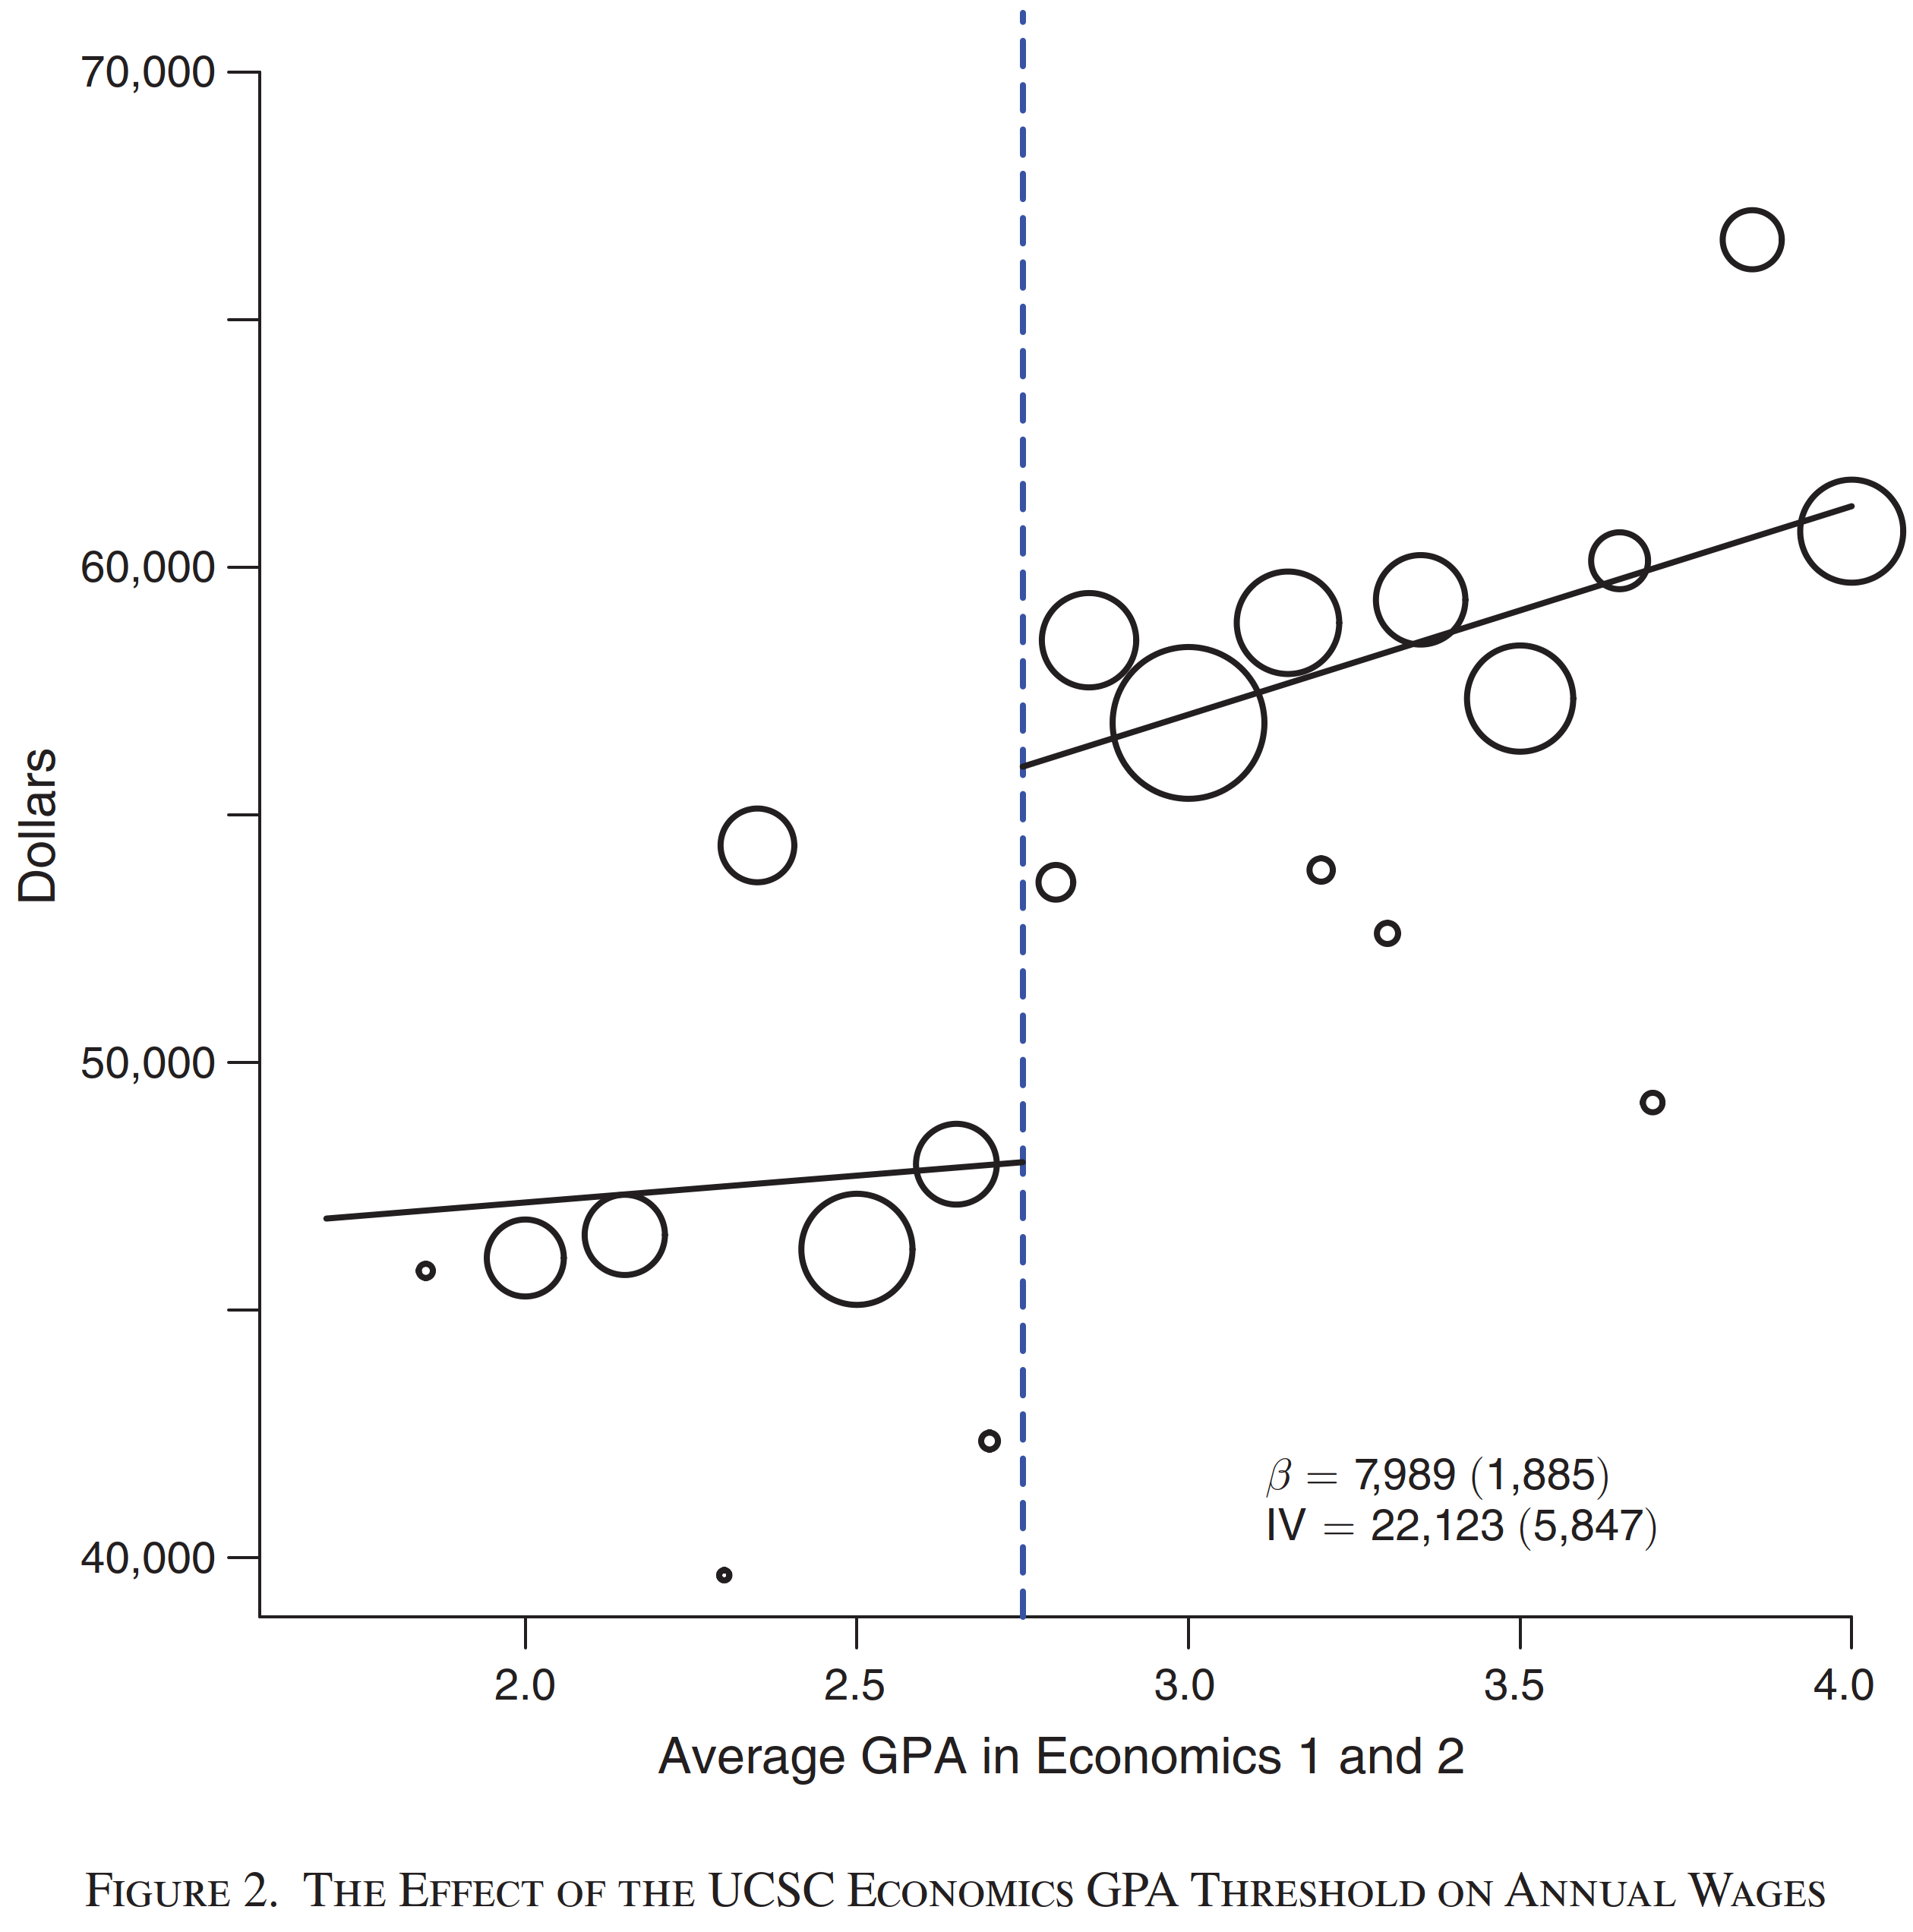
\includegraphics[width=0.60\textwidth]{figure/RD_econ_major_f2.png}
	
	
\end{frame}

\begin{frame}{Step 1: Graphical Analysis}{Covariate Balance}
	\begin{itemize}
		\item Also plot \textbf{pre-determined covariates} against the running variable
		\vspace{0.2cm}
		\item These should show \textbf{no discontinuity} at GPA = 2.8
		\vspace{0.2cm}
		\begin{itemize}
			\item SAT score, gender, URM status, zip income were fixed
			\emph{before} students knew their intro-econ GPA
			\vspace{0.2cm}
			\item A jump in any covariate would indicate that students
			above/below 2.8 differ systematically $\Rightarrow$ threat to continuity
		\end{itemize}
		\vspace{0.2cm}
		\item Bleemer \& Mehta (2022): no significant jumps in any baseline characteristic
	\end{itemize}
\end{frame}


\begin{frame}[fragile]{STATA: Step 1}{Covariate Balance}
	\begin{itemize}
		\item Example (SAT score and gender balance):
\begin{lstlisting}
binscatter sat_score gpa_econ, n(50) rd(2.8) linetype(lfit) /*
*/ title("Covariate Balance: SAT Score")
graph export figure/econ_sat.png, replace

binscatter female gpa_econ, n(50) rd(2.8) linetype(lfit)   /*
*/ title("Covariate Balance: Gender")
graph export figure/econ_female.png, replace
\end{lstlisting}
	\end{itemize}
\end{frame}


\begin{frame}[fragile]{R: Step 1}{Covariate Balance}
\begin{lstlisting}[style=r-style]
rdplot(y = data$sat_score, x = data$gpa_econ, c = cutoff,
       title = "Covariate Balance: SAT Score")
rdplot(y = data$female, x = data$gpa_econ, c = cutoff,
       title = "Covariate Balance: Gender")
\end{lstlisting}
\end{frame}


\begin{frame}{Covariate Balance}{SAT Score by GPA in Introductory Economics}
	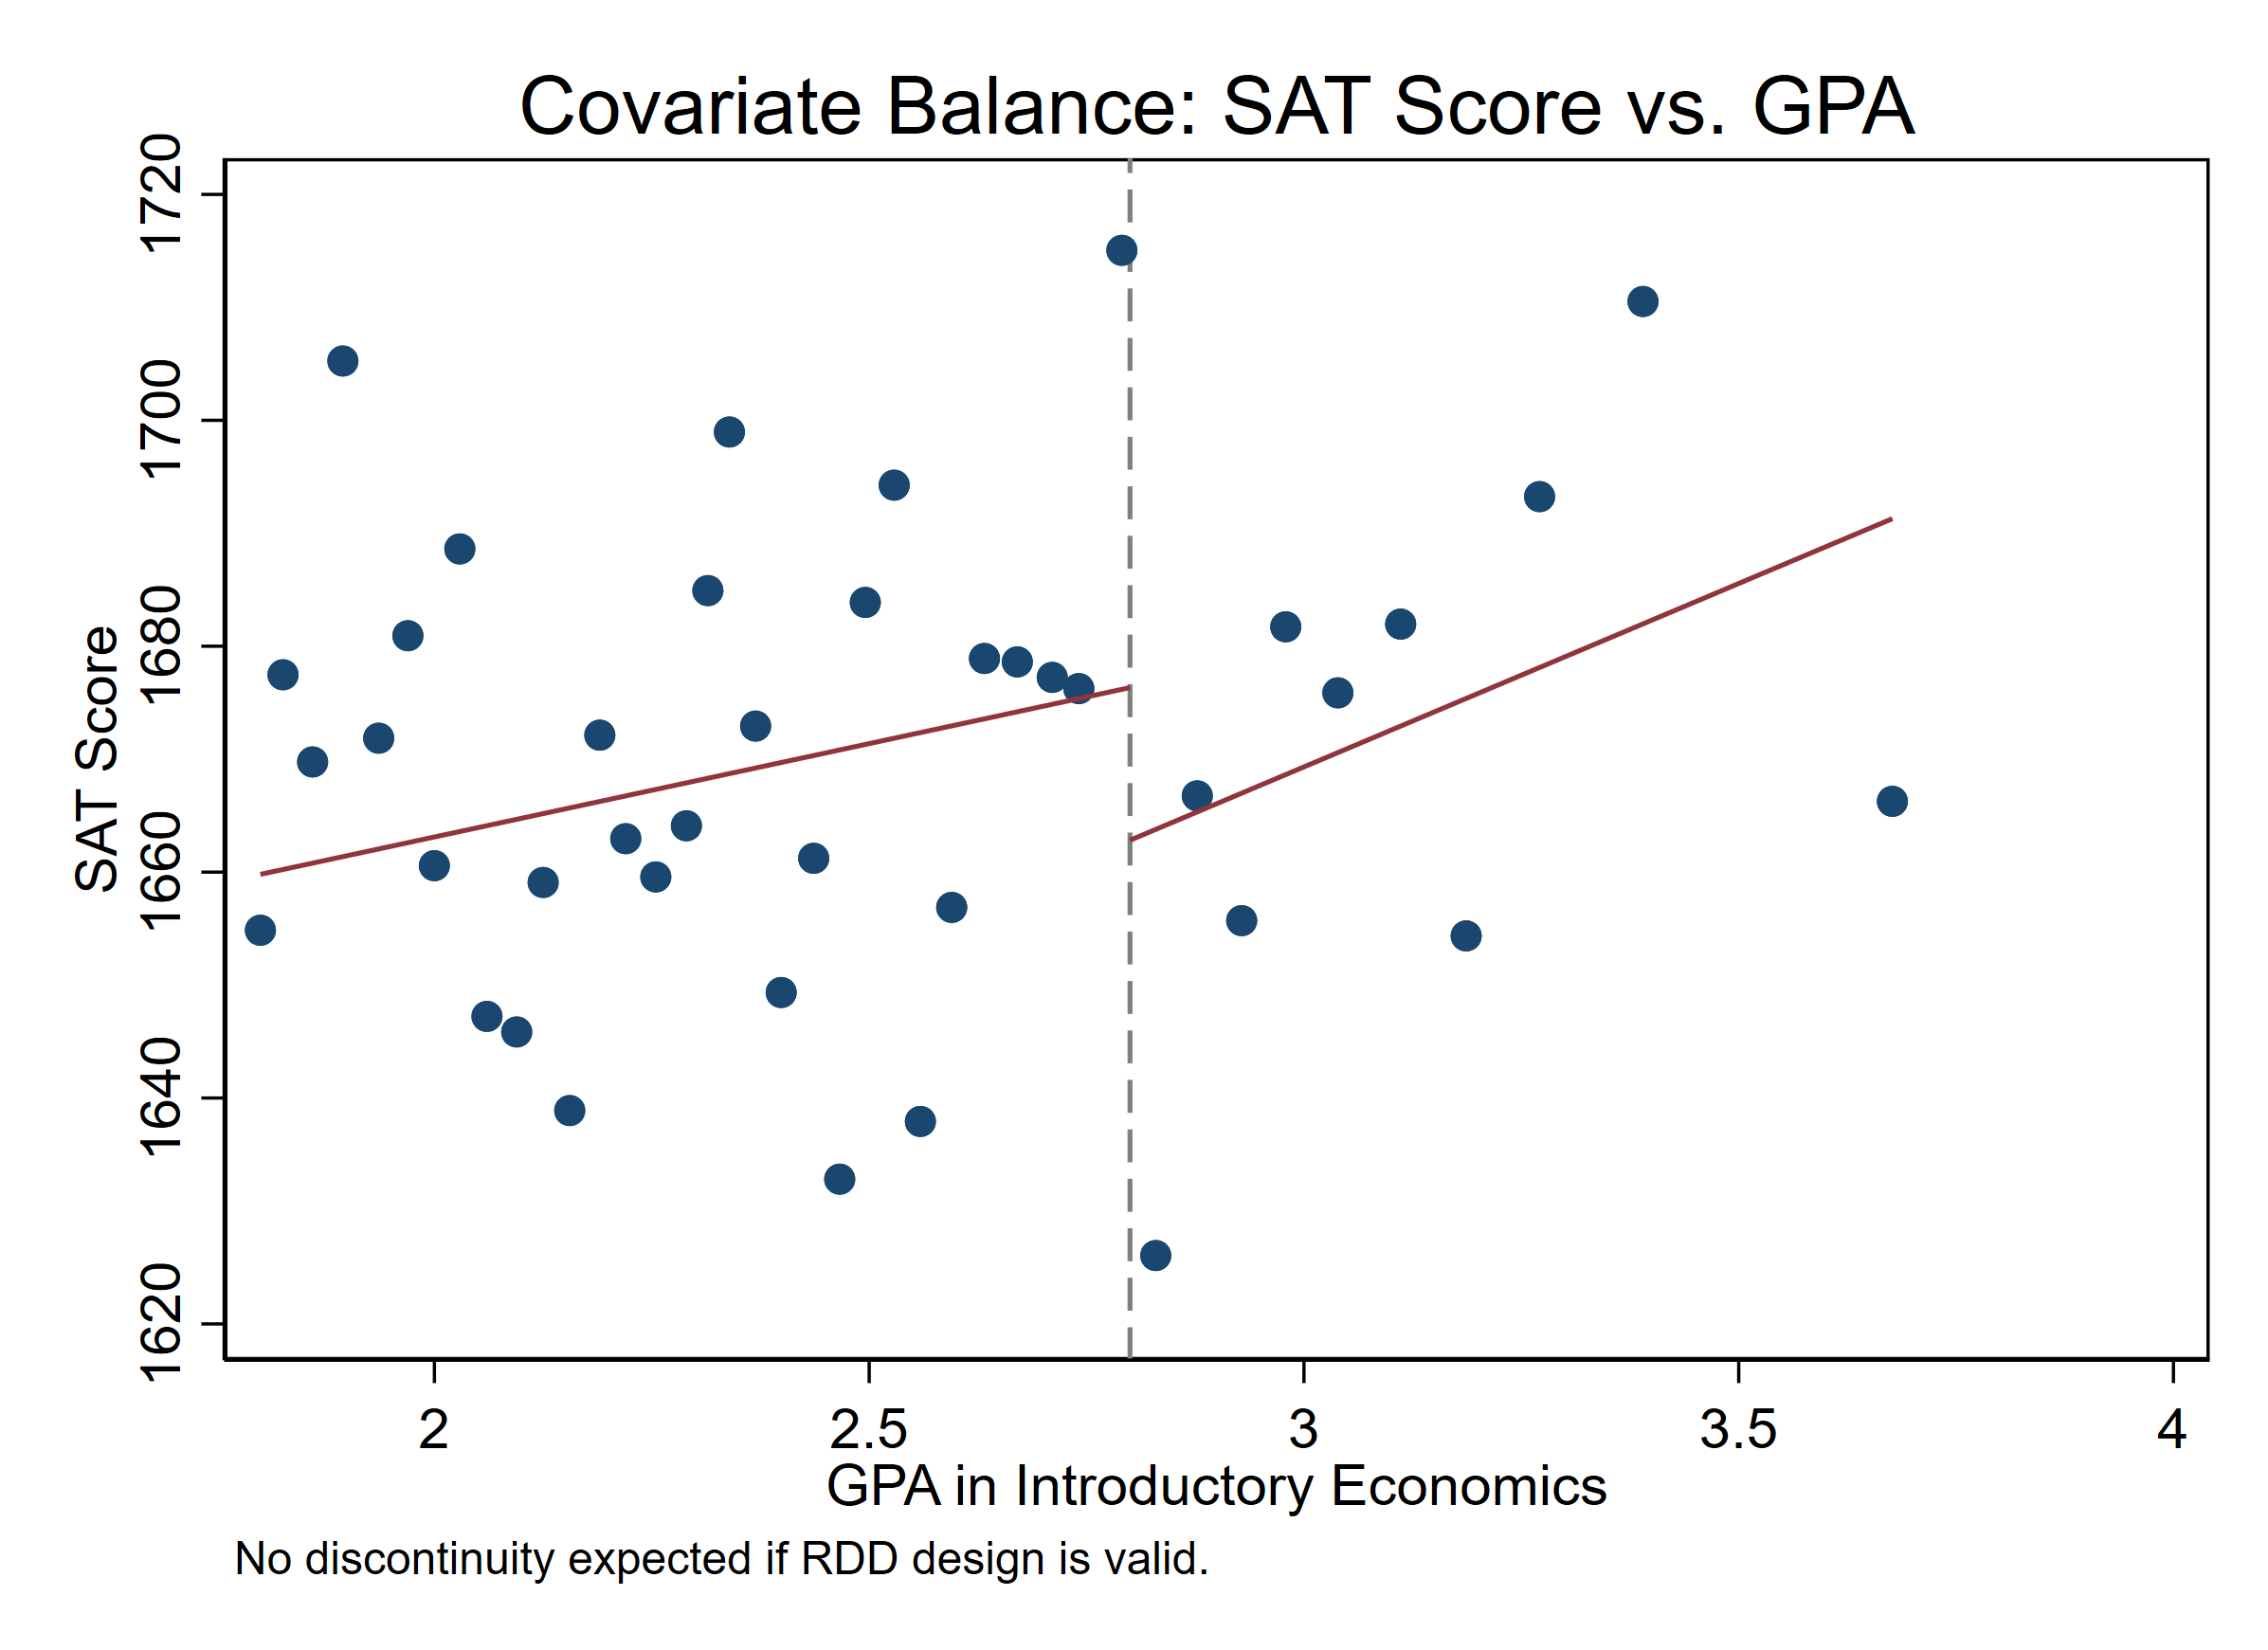
\includegraphics[width=0.9\textwidth]{figure/econ_sat.png}
\end{frame}

\begin{frame}{Covariate Balance}{Female by GPA in Introductory Economics}
	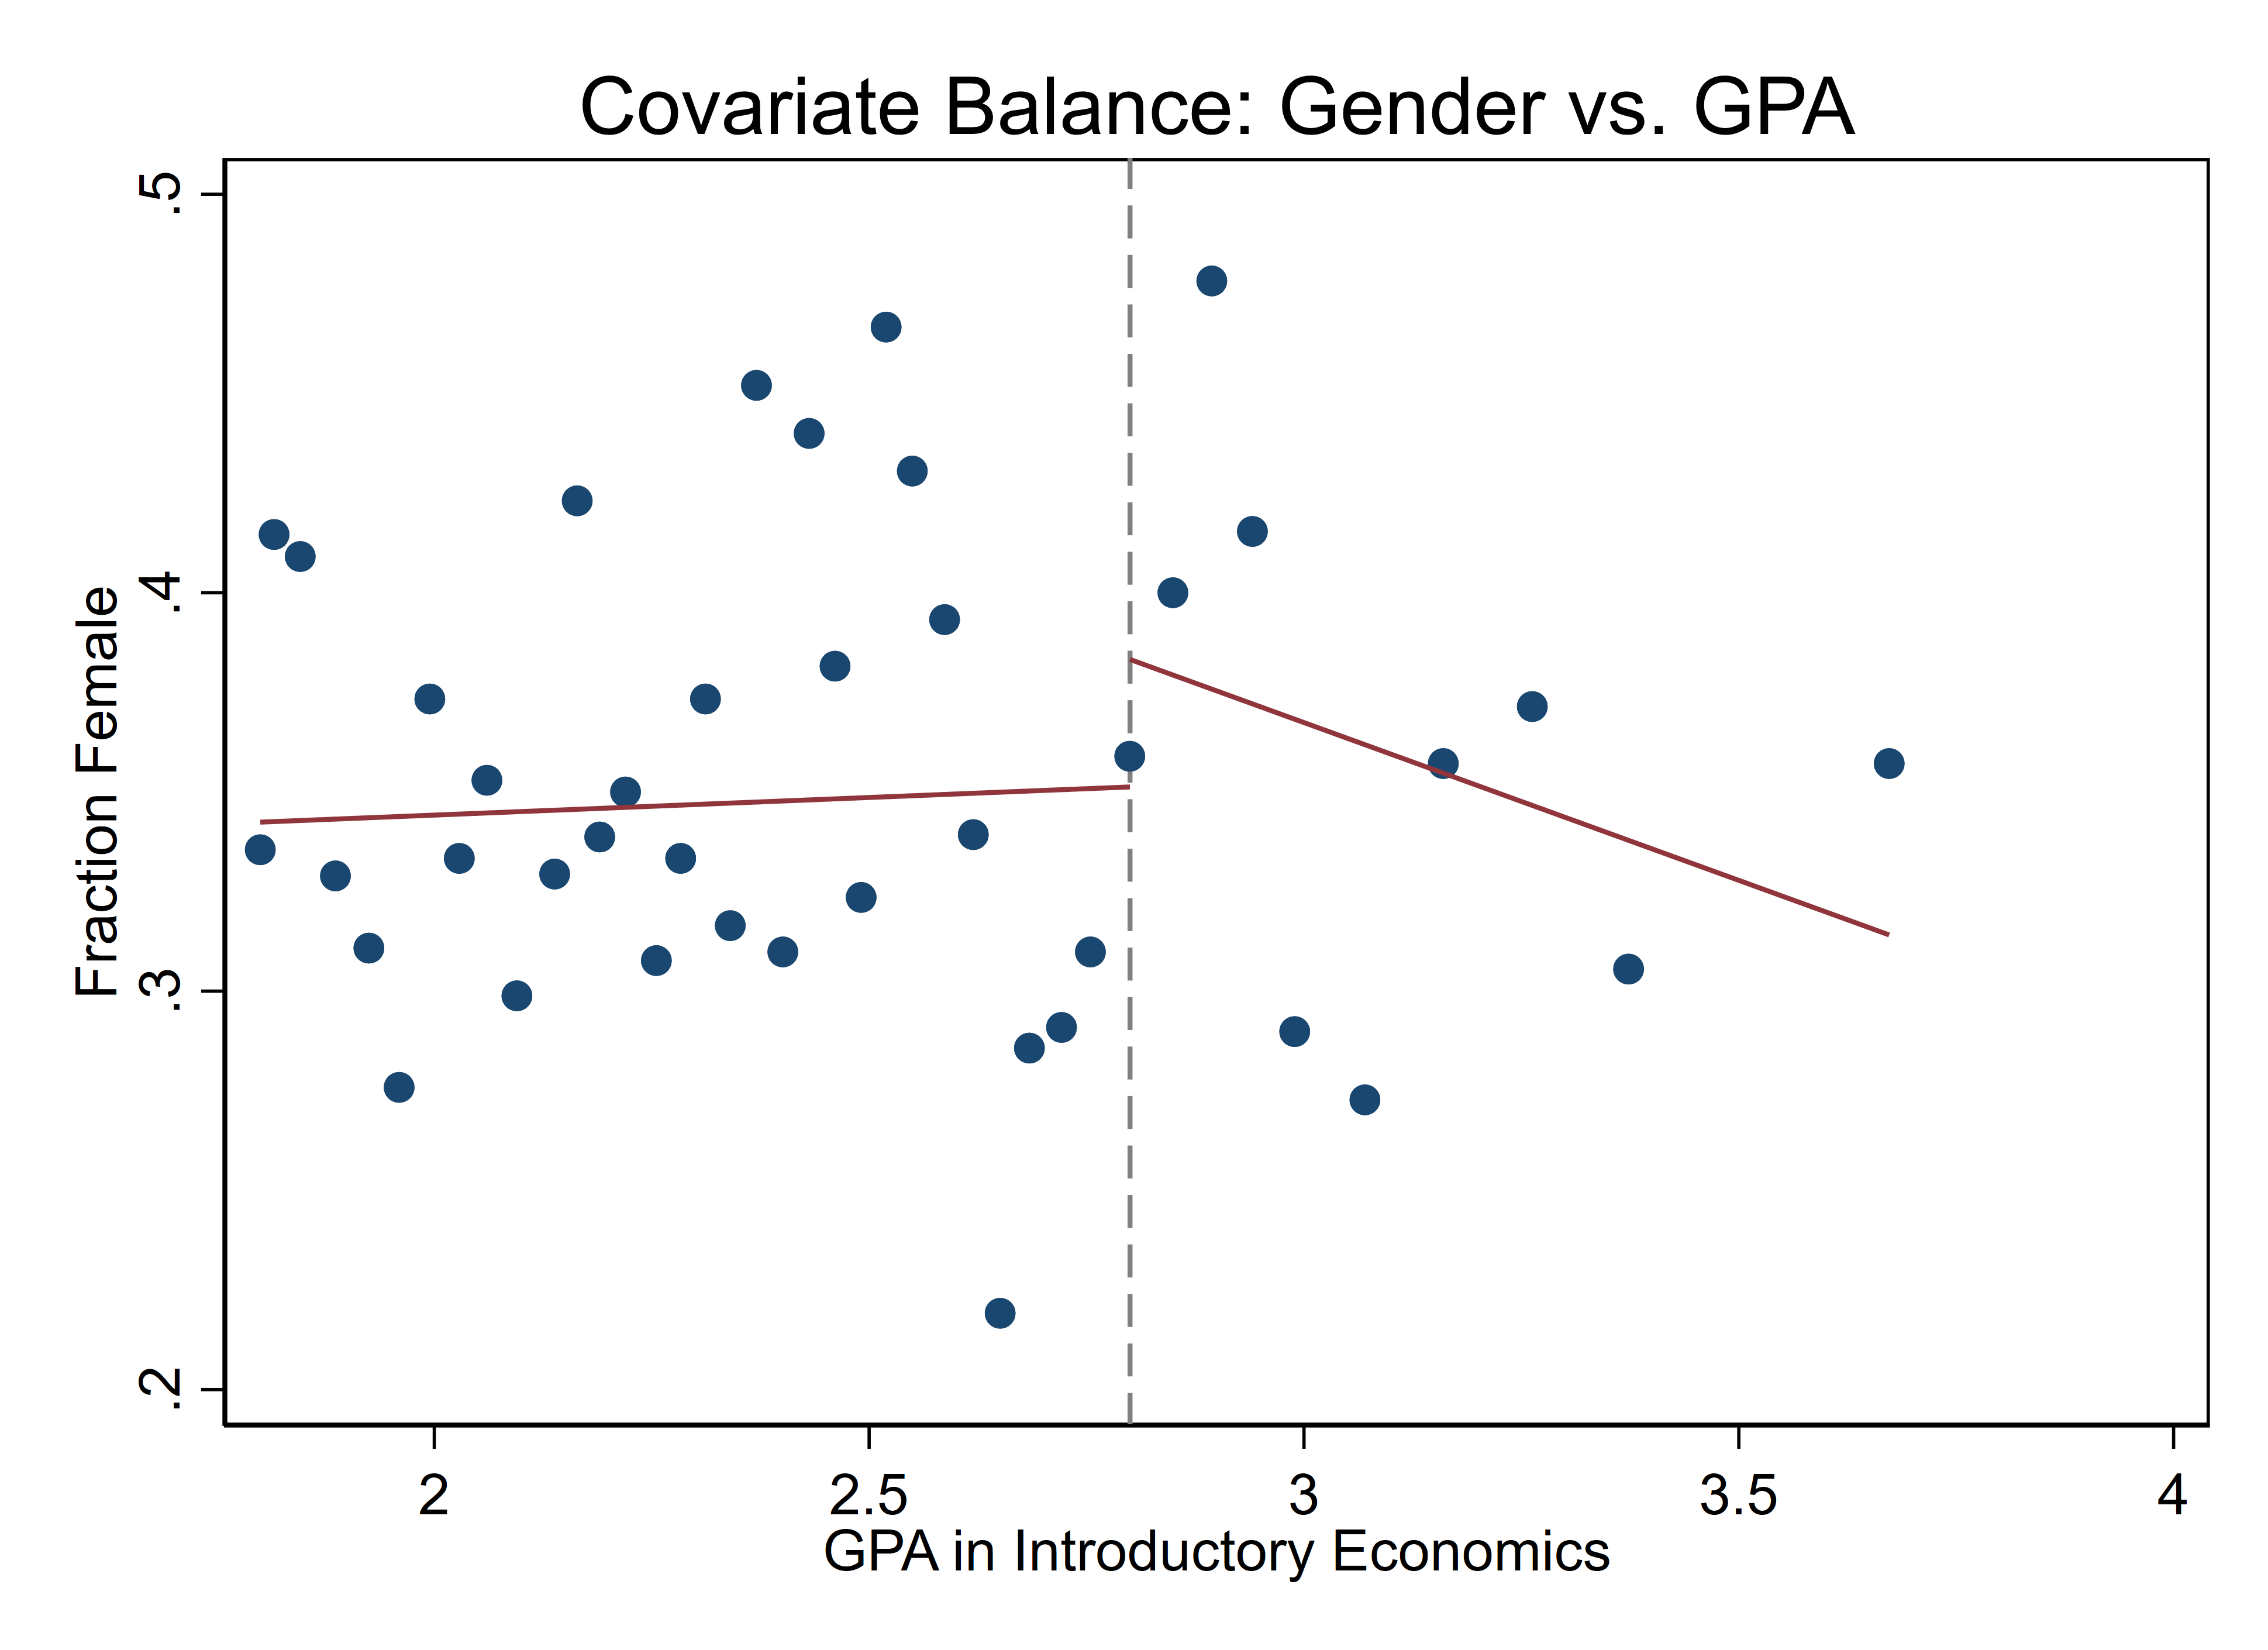
\includegraphics[width=0.9\textwidth]{figure/econ_female.png}
\end{frame}


\begin{frame}{Step 2: Test Sorting Behavior}{}
	\begin{itemize}
		\item Plot the \textbf{density of the running variable} (GPA) around the cutoff
		\vspace{0.2cm}
		\item If students can \textbf{manipulate} their GPA to just exceed 2.8
		(e.g.\ by disputing grades or retaking the exam), we would see:
		\begin{itemize}
			\vspace{0.2cm}
			\item A spike in the density \emph{just above} GPA = 2.8
			\vspace{0.2cm}
			\item A dip \emph{just below}
		\end{itemize}
		\vspace{0.2cm}
		\item $H_0$: no density discontinuity at the cutoff
		\vspace{0.2cm}
		\item Non-rejection ($p > 0.05$) supports the RDD validity assumption
		\vspace{0.2cm}
		\item Bleemer \& Mehta (2022): no evidence of manipulation at GPA = 2.8
	\end{itemize}
\end{frame}


\begin{frame}[fragile]{STATA: Step 2}{Sorting Test}
	\begin{itemize}
		\item Syntax:
\begin{lstlisting}
rddensity runvar [if] [in] [, options]
\end{lstlisting}
		\item Example:
\begin{lstlisting}
* Option A: rddensity (Cattaneo, Jansson, Ma 2020)
rddensity gpa_econ, c(2.8) all plot
graph export figure/econ_density.png, replace

* Option B: McCrary (2008) DCdensity
DCdensity gpa_econ, breakpoint(2.8) generate(Xj Yj r0 fhat se_fhat)
drop Xj Yj r0 fhat se_fhat
\end{lstlisting}
		\vspace{0.2cm}
		\item \textbf{gpa\_econ}: running variable whose density we test
		\vspace{0.2cm}
		\item \textbf{c(2.8)}: cutoff value
	\end{itemize}
\end{frame}


\begin{frame}[fragile]{R: Step 2}{Sorting Test}
\begin{lstlisting}[style=r-style]
library(rddensity)
# H0: no density discontinuity at GPA = 2.8
# p-value > 0.05 -> no evidence of manipulation -> RDD valid
dens_test <- rddensity(X = data$gpa_econ, c = cutoff)
summary(dens_test)
rdplotdensity(dens_test, data$gpa_econ,
              title = "McCrary Test: GPA Density at Cutoff")
\end{lstlisting}
\end{frame}


\begin{frame}{Test Sorting Behavior}{}
	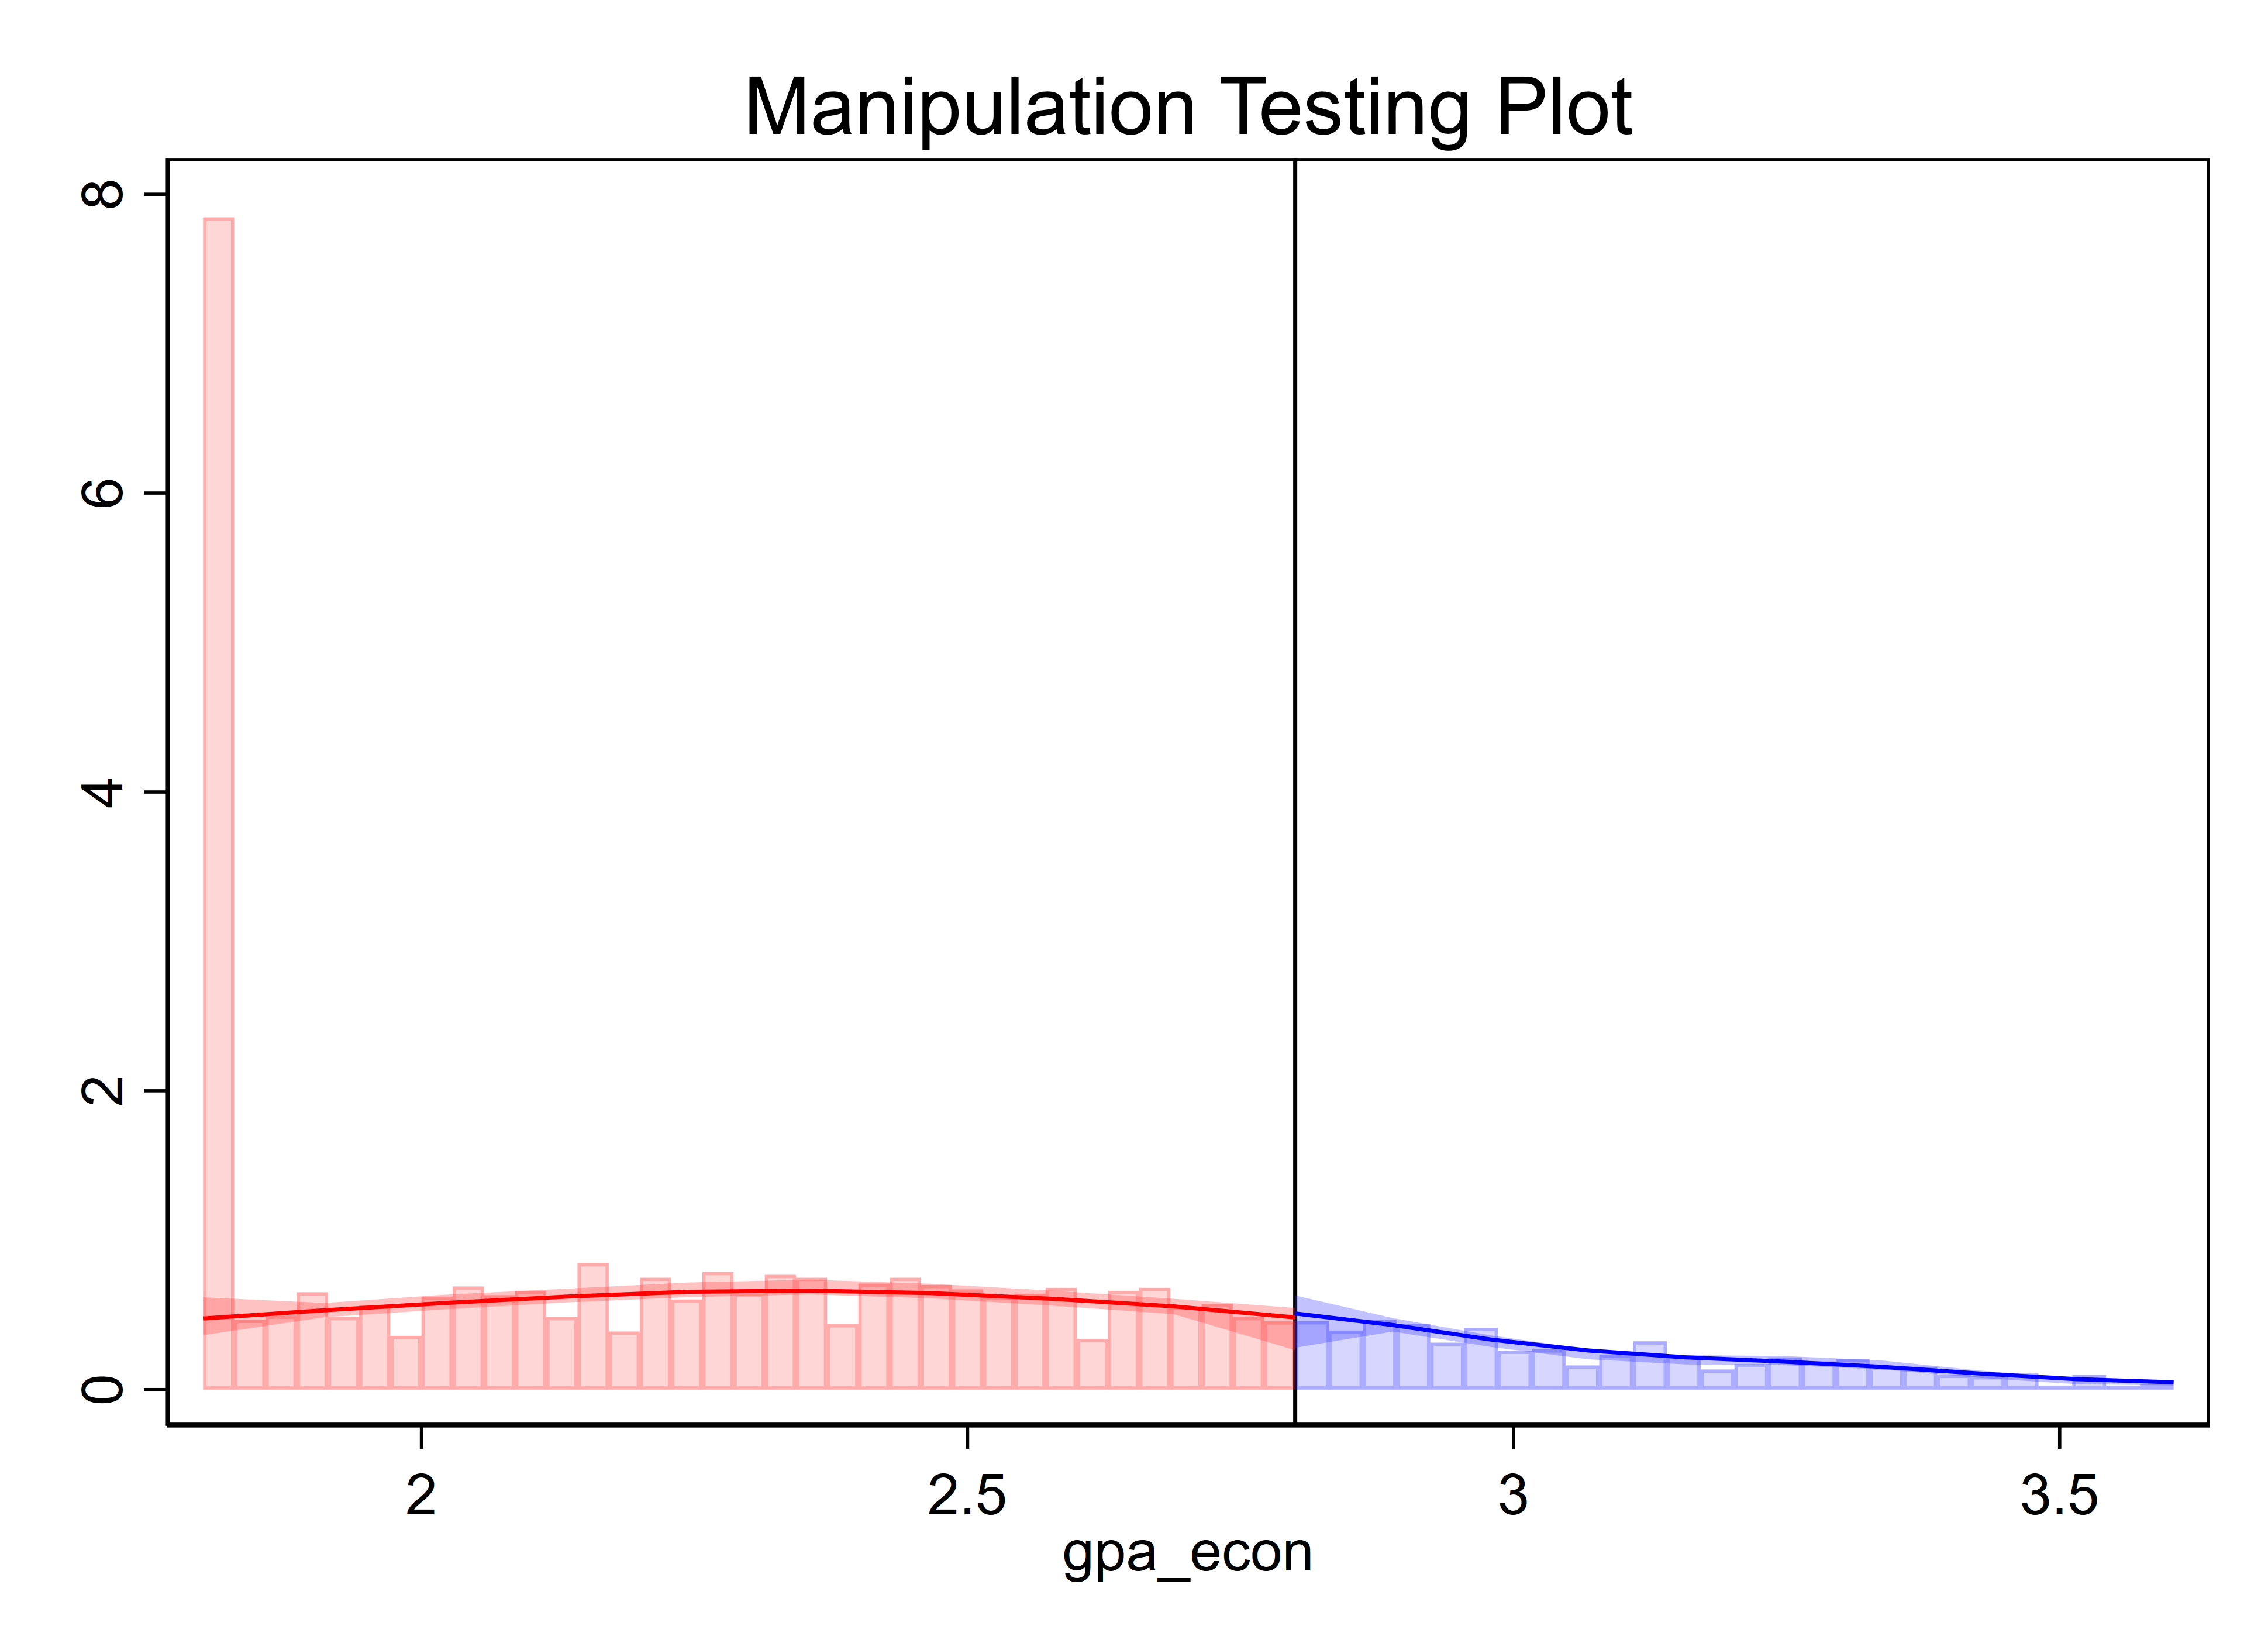
\includegraphics[width=0.9\textwidth]{figure/econ_density.png}
\end{frame}


\begin{frame}{Step 3: Preparation for Estimation}{}
	\begin{itemize}
		\item Generate centered running variable and interaction terms:
		\vspace{0.2cm}
		\begin{itemize}
			\item \textbf{gpa\_c}: $\tilde{A}_i = A_i - 2.8$, centered running variable (= 0 at cutoff)
			\vspace{0.2cm}
			\item \textbf{gpa\_c2}: $\tilde{A}_i^2$, for quadratic robustness check
			\vspace{0.2cm}
			\item \textbf{above}: $Z_i = \mathbf{1}[A_i \geq 2.8]$ (already in dataset)
			\vspace{0.2cm}
			\item \textbf{above\_gpa\_c}: $Z_i \cdot \tilde{A}_i$, allows slope to differ on each side
			\vspace{0.2cm}
			\item \textbf{above\_gpa\_c2}: $Z_i \cdot \tilde{A}_i^2$, for quadratic specification
		\end{itemize}
		\vspace{0.2cm}
		\item Also define \textbf{data\_emp}: subsample of employed workers (for wage regressions)
	\end{itemize}
\end{frame}


\begin{frame}[fragile]{STATA: Step 3}{Preparation for Estimation}
\begin{lstlisting}
gen gpa_c        = gpa_econ - 2.8
gen gpa_c2       = gpa_c^2
gen above_gpa_c  = above * gpa_c
gen above_gpa_c2 = above * gpa_c2
\end{lstlisting}
\end{frame}


\begin{frame}[fragile]{R: Step 3}{Preparation for Estimation}
\begin{lstlisting}[style=r-style]
data <- data |>
  mutate(gpa_c = gpa_econ - cutoff, gpa_c2 = gpa_c^2,
         above_gpa_c = above * gpa_c, above_gpa_c2 = above * gpa_c^2)
data_emp <- data |> filter(employed_1718 == 1, !is.na(logwage_1718))
\end{lstlisting}
\end{frame}


\begin{frame}{Step 4: Parametric Estimation}{First Stage, Reduced Form, and 2SLS}
	\begin{itemize}
		\item Estimate three regressions; LATE = Reduced Form / First Stage
		\vspace{0.2cm}
		\begin{itemize}
			\item \textbf{First Stage}: effect of crossing GPA 2.8 on economics enrollment
			\begin{equation*}
				D_i = \alpha_1 + \rho_1 Z_i + \beta_1\tilde{A}_i + \delta_1 Z_i\tilde{A}_i + \upsilon_i
			\end{equation*}
			\vspace{0.1cm}
			\item \textbf{Reduced Form} (Intent-to-Treat): effect of crossing cutoff on wages
			\begin{equation*}
				Y_i = \alpha_2 + \rho_2 Z_i + \beta_2\tilde{A}_i + \delta_2 Z_i\tilde{A}_i + \eta_i
			\end{equation*}
			\vspace{0.1cm}
			\item \textbf{Fuzzy IV (2SLS)}: instrument $D_i$ with $Z_i$ to recover LATE $= \rho_2/\rho_1$
		\end{itemize}
		\vspace{0.2cm}
		\item Bleemer \& Mehta (2022) simulated data:
		$\hat{\rho}_1 \approx 0.36$, $\hat{\rho}_2 \approx 0.14$,
		LATE $\approx 0.38$ (46\% wage premium)
	\end{itemize}
\end{frame}


\begin{frame}[fragile]{STATA: Step 4}{First Stage and Reduced Form}
\begin{lstlisting}
* First stage: Z_i -> D_i
reg econ_major above gpa_c above_gpa_c, cl(gpa_c)
display "First stage jump: " _b[above]

* Reduced form: Z_i -> Y_i  (Intent-to-Treat)
reg logwage_1718 above gpa_c above_gpa_c if employed_1718, cl(gpa_c)
display "Reduced form: " _b[above]

* Manual LATE = Reduced Form / First Stage
quietly reg econ_major above gpa_c above_gpa_c, cl(gpa_c)
local fs_coef = _b[above]
quietly reg logwage_1718 above gpa_c above_gpa_c if employed_1718, cl(gpa_c)
display "LATE = " _b[above] / `fs_coef'
\end{lstlisting}
\end{frame}


\begin{frame}[fragile]{STATA: Step 4}{Fuzzy RDD --- 2SLS (LATE)}
\begin{lstlisting}
* Fuzzy RDD: 2SLS
* Syntax: (econ_major = above) instruments D_i with Z_i
ivregress 2sls logwage_1718 gpa_c above_gpa_c  /*
*/     (econ_major = above) if employed_1718, vce(cl gpa_c)
display "LATE (2SLS): " _b[econ_major]

* OLS (biased upward due to ability selection -- for comparison)
* Unobserved ability -> both major choice and wages
reg logwage_1718 econ_major gpa_c above_gpa_c  /*
*/     if employed_1718, cl(gpa_c)
* OLS coefficient on econ_major > LATE (upward bias)
\end{lstlisting}
\end{frame}


\begin{frame}[fragile]{R: Step 4}{First Stage, Reduced Form, 2SLS}
\begin{lstlisting}[style=r-style]
library(AER)
# First stage
fs <- lm(econ_major ~ above + gpa_c + above_gpa_c, data = data)
cat("First stage:", round(coef(fs)["above"], 4), "\n")
# Reduced form (ITT)
rf <- lm(logwage_1718 ~ above + gpa_c + above_gpa_c, data = data_emp)
cat("Reduced form:", round(coef(rf)["above"], 4), "\n")
cat("Manual LATE:", round(coef(rf)["above"]/coef(fs)["above"], 4), "\n")
# Fuzzy IV (2SLS)
fuzzy_iv <- ivreg(
  logwage_1718 ~ econ_major + gpa_c + above_gpa_c |
                 above      + gpa_c + above_gpa_c, data = data_emp)
cat("LATE (2SLS):", round(coef(fuzzy_iv)["econ_major"], 4), "\n")
# OLS (biased -- for comparison)
ols <- lm(logwage_1718 ~ econ_major + gpa_c + above_gpa_c, data = data_emp)
cat("OLS:", round(coef(ols)["econ_major"], 4), "(expect > LATE)\n")
\end{lstlisting}
\end{frame}

\begin{frame}{Empirical Example: Bleemer \& Mehta (2022)}{Key Findings}
	\begin{itemize}
		\item \textbf{Large Returns}: Majoring in economics caused:
							\vspace{0.2cm}
		\begin{itemize}
			\item 46\% increase in early-career wages (\$22,000)
								\vspace{0.2cm}
			\item Similar effects for male and female students
								\vspace{0.2cm}
			\item Possibly larger effects for URM students
											\vspace{0.2cm}
					\begin{itemize}
			\item URM: Underrepresented Minority includes Black, Hispanic, and Native American students
					\end{itemize}
		\end{itemize}
		
		\vspace{0.2cm}
%		\item \textbf{Important Implications}:
%		\begin{itemize}
%			\item Major choice is first-order determinant of returns to college
%			\item Returns primarily through industry sorting
%			\item University policies affecting major access have important mobility implications
%			\item Wage differences by major approximate causal effects
%		\end{itemize}
	\end{itemize}
\end{frame}

\begin{frame}{Step 5: Nonparametric Estimation}{\texttt{rdrobust} with \texttt{fuzzy()}}
	\begin{itemize}
		\item \texttt{rdrobust} with \texttt{fuzzy()} computes LATE directly
		\begin{itemize}
			\vspace{0.2cm}
			\item Uses $Z_i$ as instrument for $D_i$ automatically
			\vspace{0.2cm}
			\item Data-driven MSE-optimal bandwidth
			\vspace{0.2cm}
			\item Bias-corrected, robust confidence intervals
		\end{itemize}
		\vspace{0.2cm}
		\item Run three \texttt{rdrobust} calls in the fuzzy case:
		\begin{enumerate}
			\vspace{0.2cm}
			\item First stage: \texttt{rdrobust econ\_major gpa\_econ, c(2.8)}
			\vspace{0.2cm}
			\item Reduced form: \texttt{rdrobust logwage \ldots, c(2.8)}
			\vspace{0.2cm}
			\item LATE: \texttt{rdrobust logwage \ldots, c(2.8) fuzzy(econ\_major)}
		\end{enumerate}
	\end{itemize}
\end{frame}


\begin{frame}[fragile]{STATA: Step 5}{Nonparametric Estimation --- rdrobust}
\begin{lstlisting}
* First stage (sharp RDD on treatment take-up)
rdrobust econ_major gpa_econ, c(2.8) kernel(tri) all

* Reduced form
rdrobust logwage_1718 gpa_econ if employed_1718, c(2.8) kernel(tri) all

* Fuzzy RDD: LATE
* fuzzy() specifies the actual treatment D_i
rdrobust logwage_1718 gpa_econ if employed_1718, /*
*/    c(2.8) fuzzy(econ_major) kernel(tri) all

* Covariate balance tests (all p-values should be > 0.05)
foreach var in sat_score female urm zip_income {
    rdrobust `var' gpa_econ, c(2.8) kernel(tri)
}
\end{lstlisting}
\end{frame}


\begin{frame}[fragile]{R: Step 5}{Nonparametric Estimation --- rdrobust}
\begin{lstlisting}[style=r-style]
# First stage
summary(rdrobust(data$econ_major, data$gpa_econ,
                 c = cutoff, kernel = "tri", all = TRUE))
# Reduced form
summary(rdrobust(data_emp$logwage_1718, data_emp$gpa_econ,
                 c = cutoff, kernel = "tri", all = TRUE))
# Fuzzy RDD: LATE (fuzzy= specifies D_i; uses Z_i automatically)
rdd_fuzzy <- rdrobust(y = data_emp$logwage_1718, x = data_emp$gpa_econ,
                      fuzzy = data_emp$econ_major,
                      c = cutoff, kernel = "tri", all = TRUE)
summary(rdd_fuzzy)
# Covariate balance
for (v in c("sat_score", "female", "urm", "zip_income")) {
  b <- rdrobust(data[[v]], data$gpa_econ, c = cutoff, kernel = "tri")
  cat(v, ": p =", round(b$pv[1], 4), "\n")
}
\end{lstlisting}
\end{frame}


\begin{frame}{Step 6: Robustness Checks}{}
	\begin{itemize}
		\item \textbf{Bandwidth sensitivity}: LATE should be stable across choices of $h$
		\vspace{0.2cm}
		\begin{itemize}
			\item Bleemer \& Mehta (2022) find estimates stable from $h = 0.3$ to $h = 1.0$
		\end{itemize}
		\vspace{0.2cm}
		\item \textbf{Polynomial order}: try quadratic specification
		\vspace{0.2cm}
		\begin{itemize}
			\item Gelman \& Imbens (2019): avoid going above second-order polynomial
		\end{itemize}
		\vspace{0.2cm}
		\item \textbf{Alternative outcomes}: employment, graduate school enrollment
		\vspace{0.2cm}
		\begin{itemize}
			\item If GPA 2.8 affects wages only through economics major, other outcomes
			should respond only if they too are affected by major choice
		\end{itemize}
	\end{itemize}
\end{frame}


\begin{frame}[fragile]{STATA: Step 6}{Robustness Checks}
\begin{lstlisting}
* Bandwidth sensitivity
foreach h in 0.3 0.4 0.5 0.6 0.8 1.0 {
    quietly rdrobust logwage_1718 gpa_econ if employed_1718, /*
    */    c(2.8) h(`h') fuzzy(econ_major) kernel(tri)
    display "h=`h': LATE=" e(tau_cl) " SE=" e(se_tau_cl)
}

* Quadratic polynomial (2SLS)
ivregress 2sls logwage_1718 gpa_c gpa_c2 above_gpa_c above_gpa_c2 /*
*/     (econ_major = above) if employed_1718, vce(cl gpa_c)

* Secondary outcomes
rdrobust employed_1718 gpa_econ, c(2.8) fuzzy(econ_major) kernel(tri)
rdrobust grad_school   gpa_econ, c(2.8) fuzzy(econ_major) kernel(tri)
\end{lstlisting}
\end{frame}


\begin{frame}[fragile]{R: Step 6}{Robustness Checks}
\begin{lstlisting}[style=r-style]
# Bandwidth sensitivity
for (h in c(0.3, 0.4, 0.5, 0.6, 0.8, 1.0)) {
  rdd_h <- rdrobust(y = data_emp$logwage_1718, x = data_emp$gpa_econ,
                    fuzzy = data_emp$econ_major,
                    c = cutoff, h = h, kernel = "tri")
  cat(sprintf("h=%.1f: LATE = %.4f\n", h, rdd_h$coef[1]))
}
# Quadratic polynomial (2SLS)
fuzzy_quad <- ivreg(
  logwage_1718 ~ econ_major + gpa_c + gpa_c2 + above_gpa_c + above_gpa_c2 |
                 above      + gpa_c + gpa_c2 + above_gpa_c + above_gpa_c2,
  data = data_emp)
cat("Quadratic LATE:", round(coef(fuzzy_quad)["econ_major"], 4), "\n")
\end{lstlisting}
\end{frame}

\begin{frame}{Empirical Example: Bleemer \& Mehta (2022)}{Mechanisms: Educational Investment}
	
	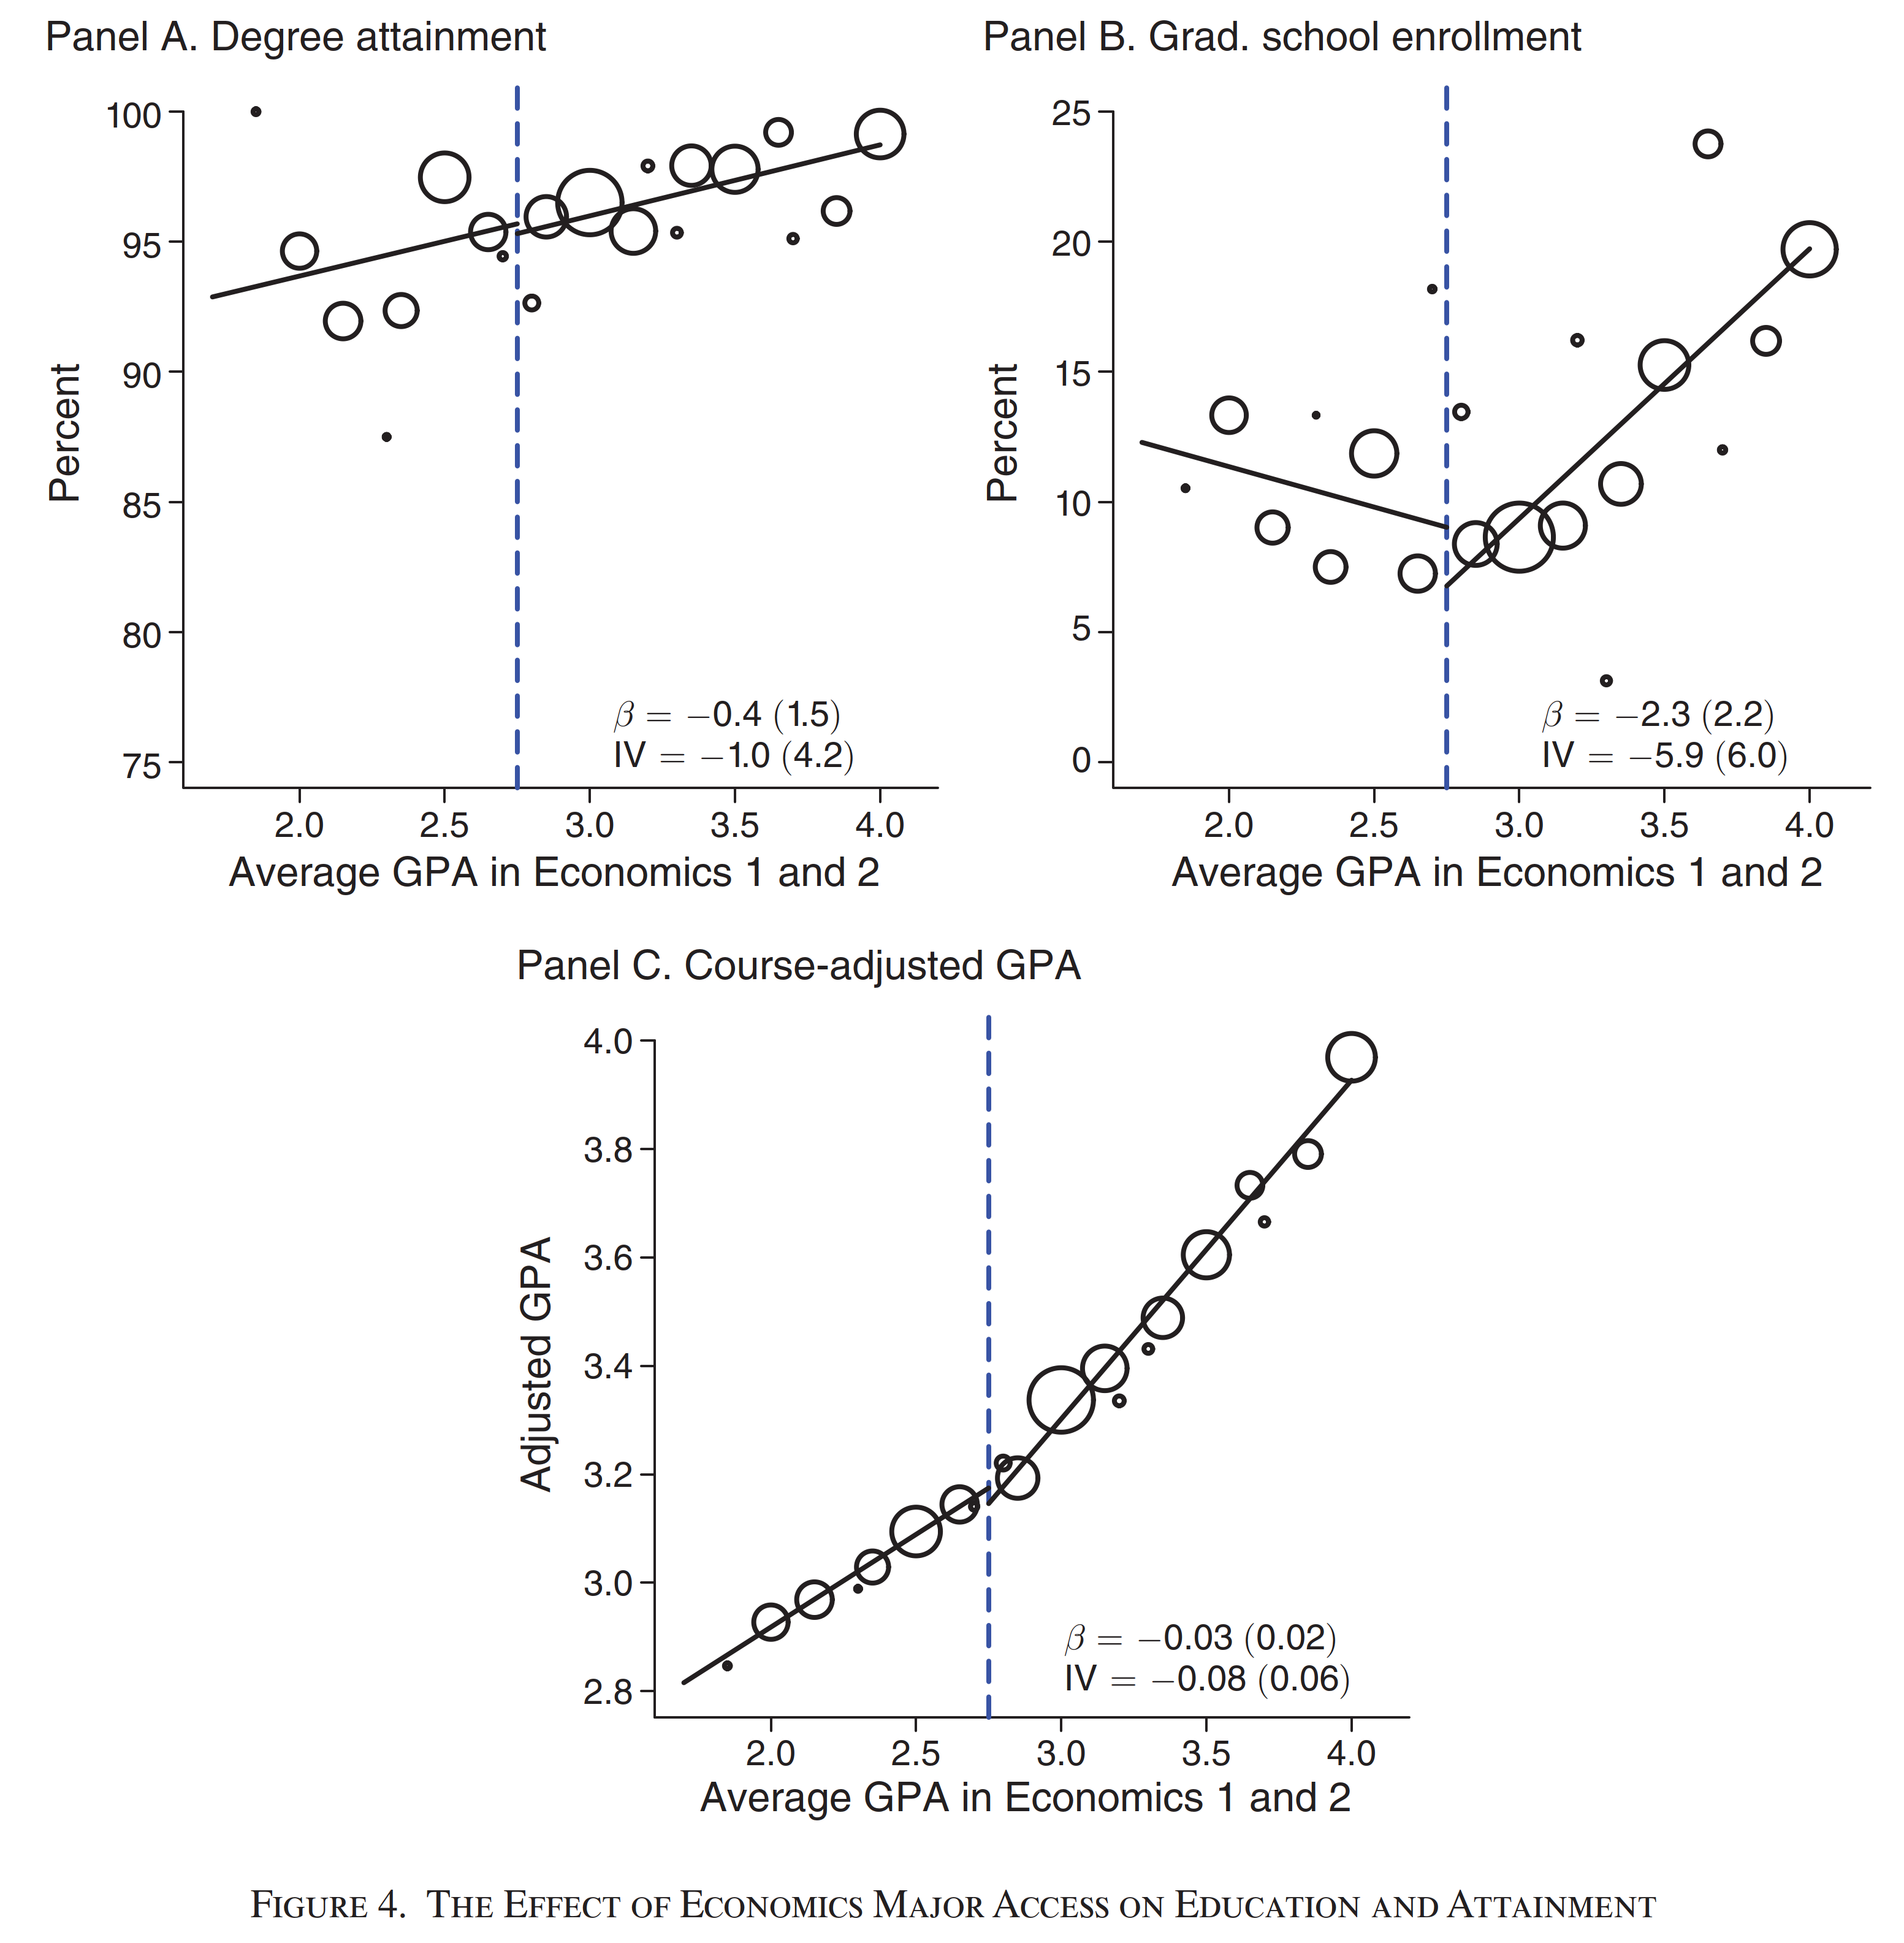
\includegraphics[width=0.7\textwidth]{figure/RD_econ_major_f3.png}
	
	
\end{frame}



\begin{frame}{Empirical Example: Bleemer \& Mehta (2022)}{Mechanisms: Industry Effects}
	
	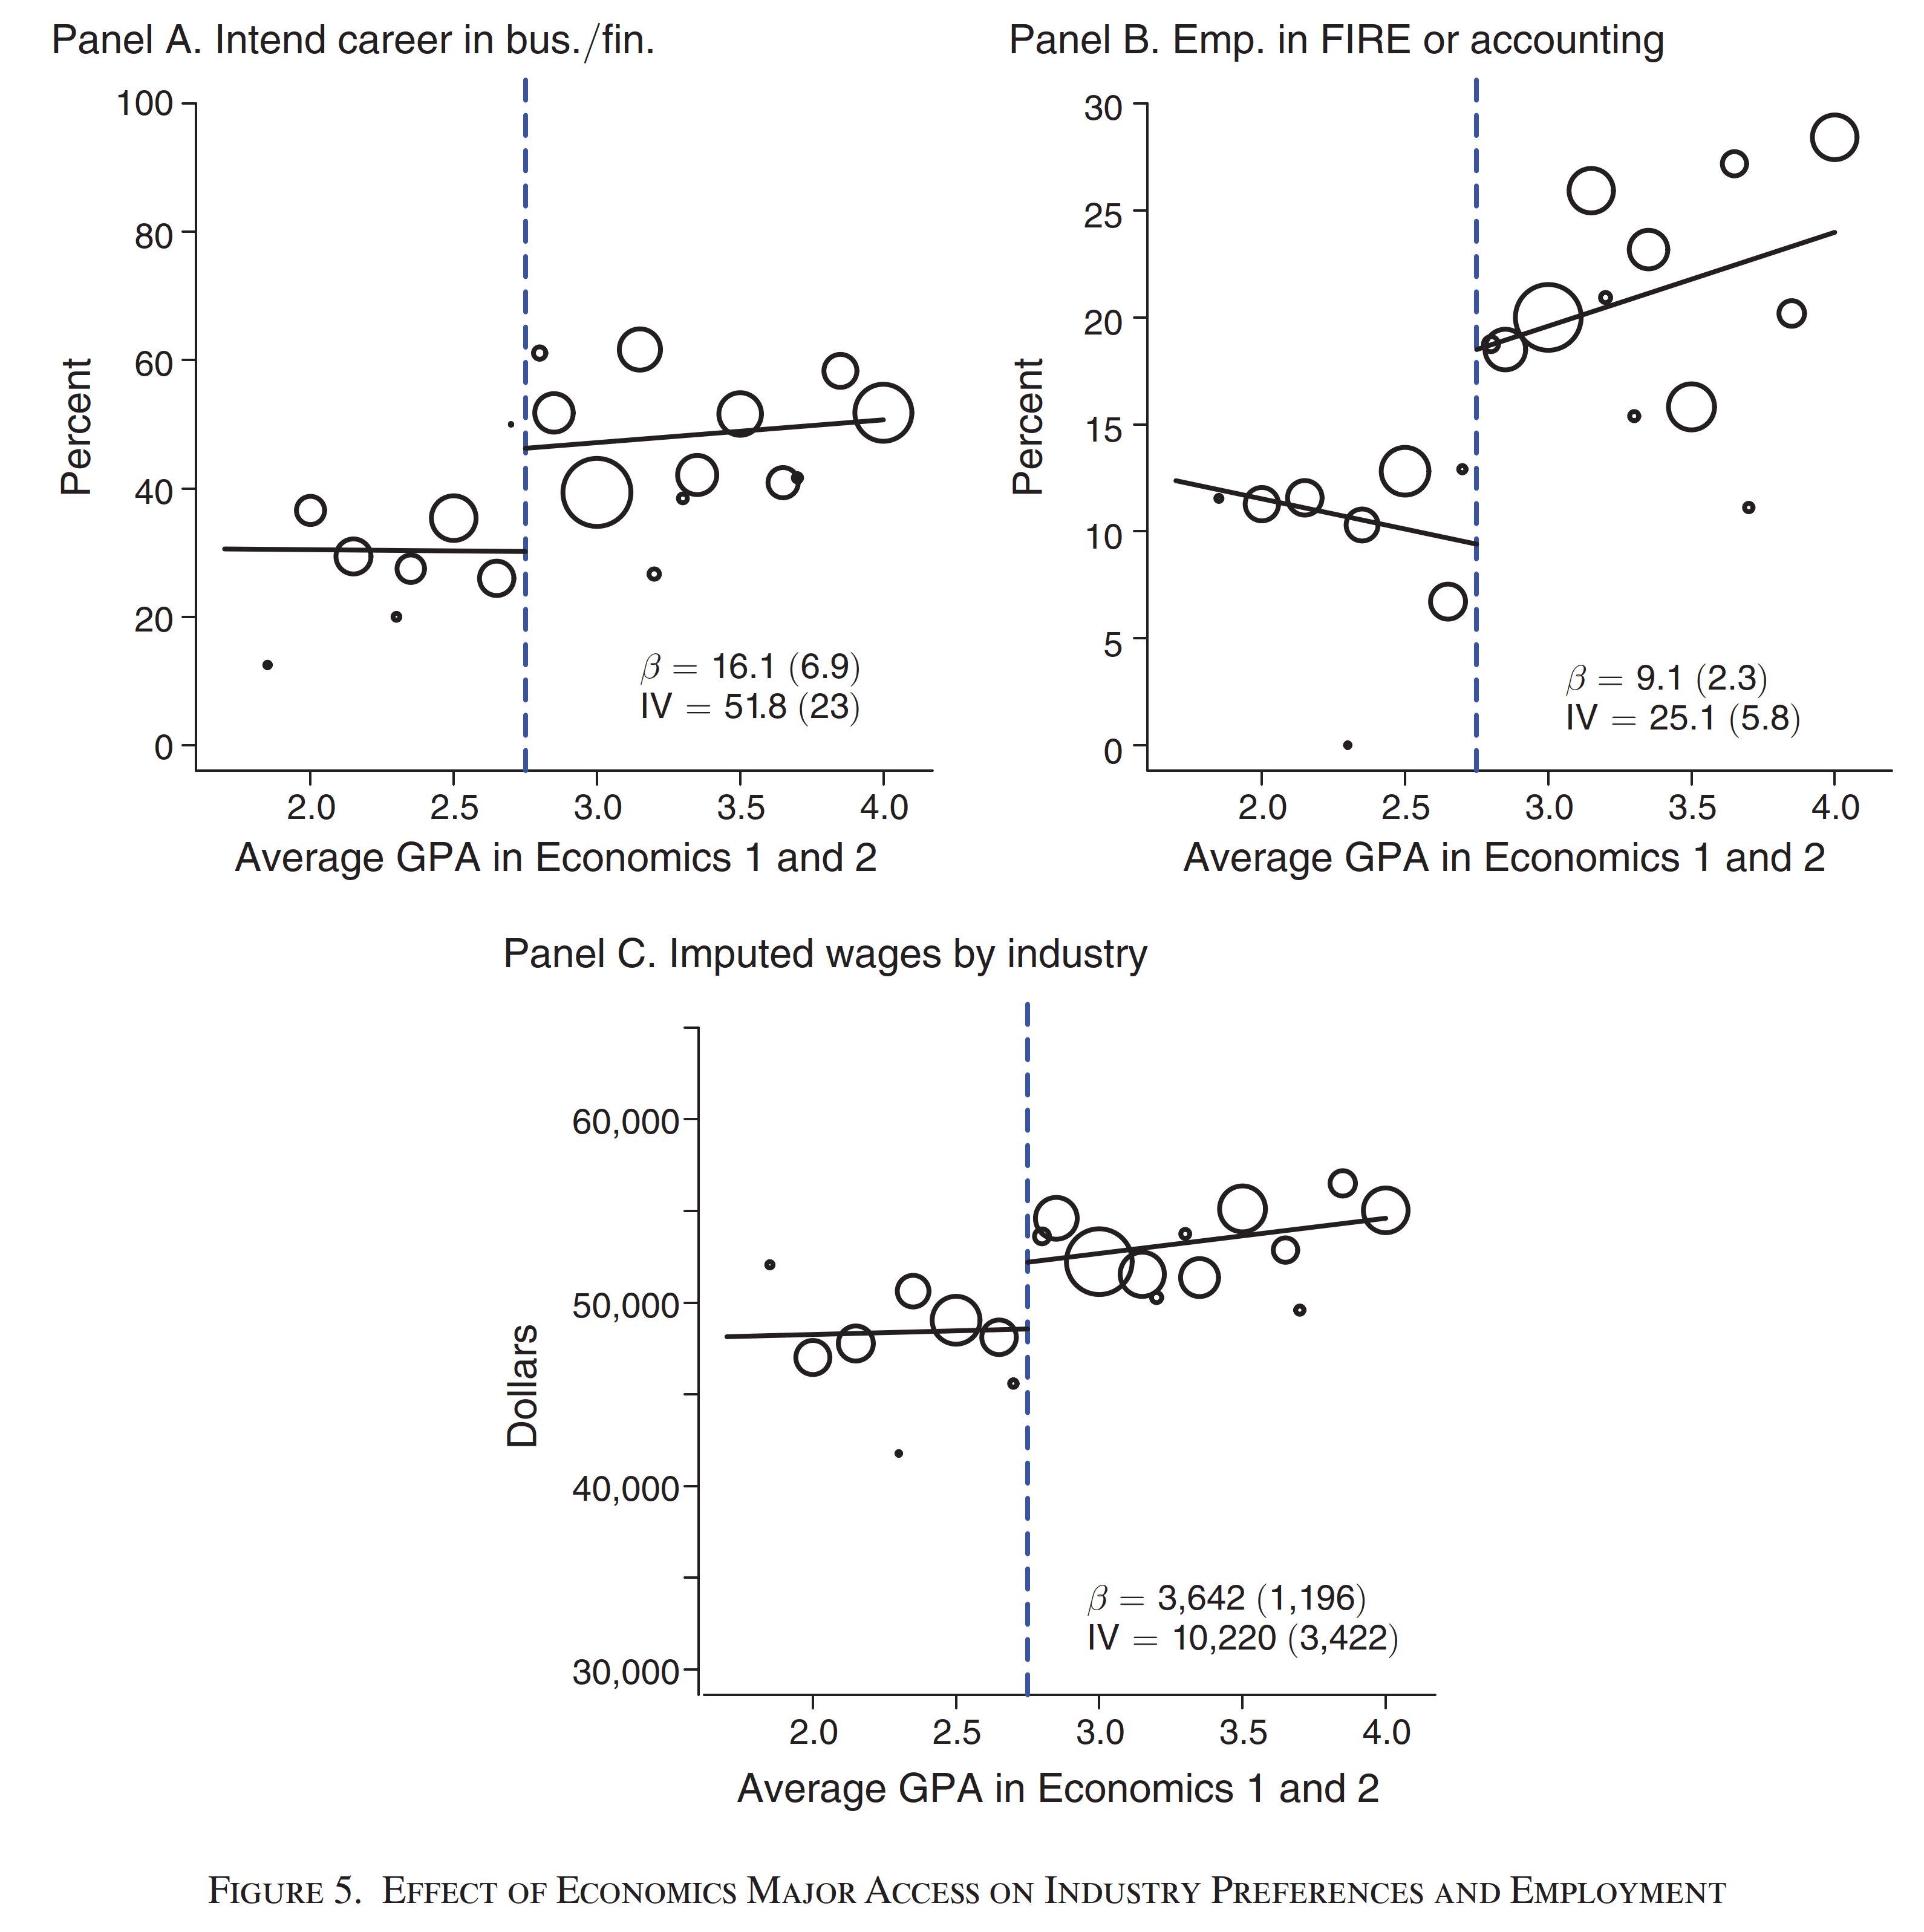
\includegraphics[width=0.7\textwidth]{figure/RD_econ_major_f4.png}
	
	
\end{frame}




\begin{frame}{Empirical Example: Bleemer \& Mehta (2022)}{Mechanisms}
	\begin{itemize}
		\item \textbf{Educational Investment}:
										\vspace{0.2cm}
		\begin{itemize}
			\item No effect on graduation rates or graduate school enrollment
											\vspace{0.2cm}
			\item No change in study time or course-adjusted grades
											\vspace{0.2cm}
			\item 13 more economics courses, 9 fewer other social science courses
											\vspace{0.2cm}
		\end{itemize}
		
		\vspace{0.2cm}
		\item \textbf{Industry Effects}:
										\vspace{0.2cm}
		\begin{itemize}
			\item 52 pp more likely to prefer business/finance careers
											\vspace{0.2cm}
			\item 25 pp more likely to work in FIRE or accounting
											\vspace{0.2cm}
			\item About half (\$10,220) of wage effect explained by industry sorting
		\end{itemize}
		
		\vspace{0.2cm}
%		\item \textbf{Observational vs. Causal Effects}:
%		\begin{itemize}
%			\item OLS estimates slightly underestimate true returns
%			\item Suggests selection bias is small in this context
%		\end{itemize}
	\end{itemize}
\end{frame}
\begin{frame}{Suggested Readings} % Changed title to reflect RDD
	\begin{itemize} 
		\item Chapter 4, \textit{Mastering 'Metrics: The Path from Cause to Effect}
		\vspace{0.2cm}
		\item Chapter 6, \textit{Mostly Harmless Econometrics: An Empiricist's Companion} % Added "An Empiricist's Companion" for completeness
		\vspace{0.2cm}
		\item Chapter 6, \textit{Causal Inference: The Mixtape}
	\end{itemize}
\end{frame}

\end{document}
